% !TEX program = xelatex
%
% miniOS 技术文档
% 模板：ElegantBook（https://github.com/ElegantLaTeX/ElegantBook）
% 编译：tectonic main.tex（或 XeLaTeX 多遍）
% 本书必须用 XeLaTeX（或 LuaLaTeX / tectonic）编译。
\RequirePackage{iftex}
\ifPDFTeX
  \errmessage{This book must be compiled with XeLaTeX (or tectonic), not pdfLaTeX.}
  \expandafter\stop
\fi
\documentclass[lang=cn,newtx,10pt,scheme=chinese,fontset=fandol,cyan,bibend=bibtex]{elegantbook}

\title{miniOS 技术文档}
\subtitle{从进程调用链到 WiFi 与 IPv4 协议栈\ ——\ T113-S3 裸机实现}

\author{Jiming Kang}
\institute{rpi\_bm / miniOS 项目}
\date{2026 年 10 月}
\version{0.1}
\bioinfo{源码}{rpi-bm（miniOS T113 / AArch64 学习内核）}

\extrainfo{进程调用链、根文件系统与 devfs、/boot FAT32、UART 控制台、XR829 WiFi 驱动、IPv4 协议栈、SMHC 主机控制器、VFS 对象模型。}

\setcounter{tocdepth}{2}
\setcounter{secnumdepth}{2}

% ---------------------------------------------------------------- 宏包
\usepackage{array,tabularx,longtable}
\usepackage{cprotect}
\usepackage{float}

% ---------------------------------------------------------------- 代码样式
% 模板默认把 listings 设成 LaTeX 语言并高亮一批 LaTeX 词，这里为 C、汇编、
% 终端和纯文本示意图分别定义样式，并清空模板的 emph 列表。
\definecolor{codekw}{RGB}{160,30,60}
\definecolor{codecm}{RGB}{110,120,130}
\definecolor{codestr}{RGB}{20,110,90}
\definecolor{codebg}{RGB}{248,249,250}

\lstdefinelanguage{armasm}{
  sensitive=false,
  morekeywords={mov,movk,movz,ldr,ldrb,str,strb,ldp,stp,adr,adrp,add,sub,subs,
    and,orr,bic,lsr,lsl,mul,cmp,cbz,cbnz,tbz,tbnz,b,bl,br,blr,ret,eret,msr,mrs,
    isb,dsb,dmb,tlbi,ic,dc,sev,wfe,wfi,svc,hvc,smc,ldar,stlr,ldaxr,stxr,nop},
  morekeywords=[2]{.global,.section,.balign,.align,.org,.word,.quad,.ascii,
    .macro,.endm,.ltorg,.p2align,.text,.data},
  morecomment=[l]{//},
  morecomment=[s]{/*}{*/},
  morestring=[b]",
}

\lstdefinestyle{xbase}{
  emph={}, emphstyle={},
  basicstyle=\ttfamily\small,
  columns=fullflexible,
  keepspaces=true,
  breaklines=true,
  frame=single,
  framerule=0.3pt,
  rulecolor=\color{structurecolor!60},
  backgroundcolor=\color{codebg},
  tabsize=4,
  showstringspaces=false,
  aboveskip=6pt, belowskip=6pt,
  xleftmargin=2pt, xrightmargin=2pt,
}
\lstdefinestyle{xc}{style=xbase, language=C,
  keywordstyle=\color{codekw}\bfseries,
  commentstyle=\color{codecm},
  stringstyle=\color{codestr},
  morekeywords={uint,uint8,uint16,uint32,uint64,uchar,pte_t,pagetable_t,
    asm,volatile,static,inline,__attribute__}}
\lstdefinestyle{xasm}{style=xbase, language=armasm,
  keywordstyle=\color{codekw}\bfseries,
  keywordstyle=[2]\color{structurecolor},
  commentstyle=\color{codecm},
  stringstyle=\color{codestr}}
\lstdefinestyle{xsh}{style=xbase, language=bash,
  keywordstyle=\color{codekw},
  commentstyle=\color{codecm},
  stringstyle=\color{codestr}}
\lstdefinestyle{xtxt}{style=xbase, language={},
  basicstyle=\ttfamily\footnotesize, columns=fixed, basewidth=0.5em}
\lstdefinestyle{xmake}{style=xbase, language=make,
  keywordstyle=\color{codekw},
  commentstyle=\color{codecm}}

\lstnewenvironment{ccode}[1][]{\lstset{style=xc,#1}}{}
\lstnewenvironment{asmcode}[1][]{\lstset{style=xasm,#1}}{}
\lstnewenvironment{shcode}[1][]{\lstset{style=xsh,#1}}{}
\lstnewenvironment{txtcode}[1][]{\lstset{style=xtxt,#1}}{}
\lstnewenvironment{makecode}[1][]{\lstset{style=xmake,#1}}{}

% 行内代码：\code{...}，下划线等特殊字符请自行转义
\newcommand{\code}[1]{\texttt{\hyphenchar\font=-1 #1}}
\setlength{\emergencystretch}{4em}
\tolerance=2000
\XeTeXlinebreaklocale "zh"
\XeTeXlinebreakskip = 0pt plus 1pt
% 制表符/几何符号/箭头/关系符号（拉丁等宽字体缺字形）交给中文字体渲染
\xeCJKDeclareCharClass{CJK}{"2500 -> "25FF, "2190 -> "2199, "2260 -> "2267}
\newcommand{\file}[1]{\texttt{\color{structurecolor!80!black}#1}}

\begin{document}

\maketitle
\frontmatter
\tableofcontents

\mainmatter

\chapter{进程创建与切换调用链}
\label{chap:process}

本章对应当前 rpi\_bm 中 AArch64（树莓派 3）学习内核的实现，说明通过内核启动函数创建用户进程、首次调度进入 EL0，以及后续异常往返的调用关系。本章最后一部分（第~\ref{sec:t113-clone} 节起）讲 T113（ARMv7-A）内核里 fork、vfork、clone 的统一实现，以及它和 xv6、Linux 的区别。后续各章转到 T113 上的 miniOS，讲文件系统、控制台与网络。

\section{总调用链}

\begin{txtcode}[basicstyle=\ttfamily\scriptsize]
kernel_main()
+-- copy_process(PF_KTHREAD, kernel_process, 0, 0)
    +-- allocate_kernel_page()                  分配 task_struct
    |   +-- task_struct.cpu_context             位于 task_struct 偏移 0
    +-- allocate_kernel_page()                  分配独立内核栈
    +-- task_pt_regs(p)
    |   +-- pt_regs                             固定放在内核栈高地址端
    +-- p->cpu_context.x19 = kernel_process     首次执行的内核函数
    +-- p->cpu_context.x20 = 0                  函数参数
    +-- p->cpu_context.pc = ret_from_fork       cpu_switch_to 的返回目标
    +-- p->cpu_context.sp = childregs           首次运行时的内核 SP

kernel_main()
+-- schedule()
    +-- _schedule()
        +-- switch_to(next)
            +-- switch_user_pgd(next->mm->pgd)  已有用户进程才切换 TTBR0_EL1
            +-- cpu_switch_to(prev, next)
                +-- 保存 prev 的 x19～x30 和 SP
                +-- 恢复 next 的 x19～x30 和 SP
                +-- ret
                    +-- ret_from_fork
                        +-- preempt_enable()
                        +-- x19 != 0
                        +-- blr x19
                            +-- kernel_process()
                                +-- launch_user_image(...)
                                    +-- allocate_kernel_page()          分配 mm_struct
                                    +-- allocate_pagetable_page()       分配用户 PGD
                                    +-- move_to_user_mode(...)
                                        +-- map_and_copy_user_code()    映射并复制用户代码
                                        +-- allocate_user_page()        映射用户栈
                                        +-- task_pt_regs(current)
                                        +-- regs->pc = 用户入口地址
                                        +-- regs->sp = 用户栈顶
                                        +-- regs->pstate = EL0t 状态
                                        +-- TTBR0_EL1 = current->mm->pgd

ret_from_fork
+-- kernel_process() 返回
    +-- ret_to_user                         位于 blr x19 后面
        +-- 从 pt_regs 读取 sp
        |   +-- SP_EL0 = pt_regs->sp
        +-- 从 pt_regs 读取 pc
        |   +-- ELR_EL1 = pt_regs->pc
        +-- 从 pt_regs 读取 pstate
        |   +-- SPSR_EL1 = pt_regs->pstate
        +-- kernel_exit 0
            +-- 恢复 x0～x30
            +-- 释放 pt_regs 栈帧
            +-- eret
                +-- EL0 用户入口
\end{txtcode}

\section{第一个用户进程}

\begin{txtcode}
kernel_main
+-- copy_process(PF_KTHREAD, kernel_process, ...)
    +-- 首次调度
        +-- ret_from_fork
            +-- kernel_process
                +-- launch_user_image("user-image-1", ...)
                    +-- move_to_user_mode
                        +-- 用户代码 VA 0x400000
                        +-- 用户栈 VA 0x07fff000～0x08000000
                        +-- ELR_EL1 = 0x400000
                        +-- SP_EL0 = 0x08000000
                        +-- TTBR0_EL1 = 该进程的用户 PGD
\end{txtcode}

\section{第二个用户进程}

\begin{txtcode}
kernel_main
+-- copy_process(PF_KTHREAD, kernel_process2, ...)
    +-- 首次调度
        +-- ret_from_fork
            +-- kernel_process2
                +-- launch_user_image("user-image-2", ...)
                    +-- move_to_user_mode
                        +-- 用户代码 VA 0x401000
                        +-- 用户栈 VA 0x07fff000～0x08000000
                        +-- ELR_EL1 = 0x401000
                        +-- SP_EL0 = 0x08000000
                        +-- TTBR0_EL1 = 该进程的用户 PGD
\end{txtcode}

两个进程可以使用相同的用户栈虚拟地址，因为各自的 \code{TTBR0\_EL1} 指向不同的用户页表，最终映射到不同物理页。

\section{系统调用调用链}

\begin{txtcode}
EL0 用户代码
+-- call_sys_xxx()
    +-- svc #0
        +-- EL0 synchronous exception
            +-- el0_sync
                +-- kernel_entry 0
                |   +-- CPU 已切换到该任务的 SP_EL1
                |   +-- 在内核栈顶部保存新的 pt_regs
                +-- el0_svc
                    +-- 根据 x8 查找 sys_call_table
                    +-- blr sys_xxx
                    +-- ret_from_syscall
                        +-- 把返回值写入 pt_regs->x0
                        +-- kernel_exit 0
                            +-- 恢复用户寄存器
                            +-- eret 返回 EL0
\end{txtcode}

\section{定时器中断和进程切换}

\begin{txtcode}
EL0 用户代码
+-- 定时器 IRQ
    +-- el0_irq
        +-- kernel_entry 0                       保存当前用户 pt_regs
        +-- handle_irq()
            +-- timer_tick()
                +-- _schedule()
                    +-- switch_to(next)
                        +-- switch_user_pgd(next->mm->pgd)
                        |   +-- TTBR0_EL1 = next 用户 PGD
                        +-- cpu_switch_to(prev, next)
                            +-- 保存 prev.cpu_context
                            +-- 恢复 next.cpu_context
                            +-- 返回到 next 原先暂停的位置

next 的异常返回路径
+-- handle_irq() 返回
    +-- kernel_exit 0
        +-- 从 next 内核栈上的 pt_regs 恢复现场
        +-- eret 返回 next 的 EL0
\end{txtcode}

\section{两类上下文的职责}

\begin{txtcode}
task_struct
+-- cpu_context
    +-- x19～x30
    +-- 内核 SP
    +-- 用途：EL1 调度切换

内核栈顶部
+-- pt_regs / TrapFrame
    +-- x0～x30
    +-- SP_EL0
    +-- ELR_EL1
    +-- SPSR_EL1
    +-- 用途：EL0 异常进入和 eret 返回
\end{txtcode}

\code{cpu\_context} 是 \code{task\_struct} 的第一个成员，因此两者起始地址相同。这是当前内核与 \code{cpu\_switch\_to} 汇编之间的软件布局约定，并非 ARM64 硬件规定。

\section{TTBR0 与 TTBR1}

\begin{txtcode}
低地址用户空间
+-- TTBR0_EL1
    +-- current->mm->pgd
        +-- 用户代码
        +-- 用户栈

高半区内核空间
+-- TTBR1_EL1
    +-- 全局 kernel_pgd
        +-- 内核代码和数据
        +-- task_struct 与内核栈的直接映射
        +-- MMIO
\end{txtcode}

调度用户进程时只需切换 \code{TTBR0\_EL1}；\code{TTBR1\_EL1} 保持指向公共内核页表。

\section{PSTATE 注意事项}

当前代码使用：

\begin{ccode}
regs->pstate = PSR_MODE_EL0t | PSR_DAIF_MASK;
\end{ccode}

这会得到 \code{0x3c0}，屏蔽 Debug、SError、IRQ 和 FIQ。若希望 EL0 用户进程能够被定时器正常抢占，应改为：

\begin{ccode}
regs->pstate = PSR_MODE_EL0t;
\end{ccode}

即初始 \code{SPSR\_EL1} 为 \code{0x0}。

\section{T113（ARMv7-A）：fork、vfork 与 clone}
\label{sec:t113-clone}

前面各节讲的是树莓派 AArch64 内核。从这一节起讲 T113 内核（Cortex-A7，ARM32）。它的进程创建写在 \code{src/kernel/sched/core.c} 里：

\begin{itemize}
  \item 用户态能用的系统调用只有 \code{fork} 和 \code{vfork}；
  \item 内核线程也走同一条路径；
  \item 三者共用一个入口 \code{t113\_kernel\_clone()}，形状对齐 Linux 的 \code{kernel\_clone()}。
\end{itemize}

\subsection{三种创建方式的语义}

\begin{table}[H]
\centering
\small
\begin{tabularx}{\linewidth}{l>{\raggedright\arraybackslash}X>{\raggedright\arraybackslash}X>{\raggedright\arraybackslash}X>{\raggedright\arraybackslash}X}
\toprule
 & fork & vfork & clone（Linux） & T113 内核线程 \\
\midrule
地址空间 & 复制一份：Linux 写时复制，T113/xv6 立即整页拷贝 & 和父进程共用同一个 mm & \code{CLONE\_VM} 决定共享还是复制 & 不需要用户地址空间，只用内核页表 \\
父进程 & 立即返回，继续运行 & 挂起，直到子进程 exec 或 exit & 带 \code{CLONE\_VFORK} 时同 vfork & 不受影响 \\
子进程返回值 & 0 & 0 & 0（线程用调用者给的新栈） & 不回用户态，直接跑 \code{fn(arg)} \\
文件描述符 & 每个 fd 加一次引用 & 同 fork & 带 \code{CLONE\_FILES} 时共享整张表 & 无 \\
典型用途 & 通用的“复制自己” & 紧接 exec 的 shell 场景，省掉一次拷贝 & 线程、容器、命名空间 & 内核后台工作 \\
T113 入口 & \code{T113\_SYS\_FORK} → \code{t113\_fork\_user()} & \code{T113\_SYS\_VFORK} → \code{t113\_vfork\_user()} & 无用户态 clone 系统调用 & \code{t113\_create\_kernel\_thread()} \\
\bottomrule
\end{tabularx}
\end{table}

fork 和 vfork 的差别只在两件事上：

\begin{itemize}
  \item 子进程有没有自己的地址空间；
  \item 父进程要不要等。
\end{itemize}

用时间线看：

\begin{txtcode}
fork:
 父 --fork()--+------------ 继续运行（拿到子 pid）----------------→
              |  复制 mm（T113: 每个用户页都 memcpy 一遍）
 子           +-- 从 fork() 返回 0 -- exec / 运行 -- exit --→ ZOMBIE
                                                         父 wait() 回收

vfork:
 父 --vfork()-+ WAITING（不被调度）                +-- 返回子 pid --→
              |  共享 mm（引用计数 +1，不拷贝）    |
 子           +-- 从 vfork() 返回 0 -- exec --------+  t113_vfork_complete()
                  （这段时间子进程在父进程的地址空间、
                    父进程的用户栈上运行）
\end{txtcode}

\subsection{统一实现：\code{t113\_kernel\_clone()}}

T113 内核用三个“创建策略”标志描述子进程怎样继承父进程的资源。它们定义在\code{src/include/t113/sched.h}，刻意和描述“已有任务是什么”的 \code{PF\_*} 分开：

\begin{table}[H]
\centering
\small
\begin{tabularx}{\linewidth}{>{\raggedright\arraybackslash}Xl>{\raggedright\arraybackslash}X>{\raggedright\arraybackslash}X}
\toprule
标志 & 值 & 含义 & Linux 对应 \\
\midrule
\code{T113\_CLONE\_VM} & 0x1 & 共享父进程 \code{mm}，不复制 & \code{CLONE\_VM} \\
\code{T113\_CLONE\_VFORK} & 0x2 & 父进程等子进程 exec/exit，必须和 VM 一起用 & \code{CLONE\_VFORK} \\
\code{T113\_CLONE\_KTHREAD} & 0x4 & 创建内核线程，忽略父 trapframe & \code{kernel\_thread()} 的 \code{PF\_KTHREAD} 路径 \\
\bottomrule
\end{tabularx}
\end{table}

三个外部入口只是不同的标志组合：

\begin{txtcode}[basicstyle=\ttfamily\scriptsize]
t113_fork_user(tf)              = t113_kernel_clone(0,                   tf, "fork-child",  0, 0)
t113_vfork_user(tf)             = t113_kernel_clone(VM | VFORK,          tf, "vfork-child", 0, 0)
                                  + t113_sched_yield()       父进程在这里让出 CPU
t113_create_kernel_thread(n,f,a)= t113_kernel_clone(KTHREAD,             0,  n,             f, a)
\end{txtcode}

\code{t113\_kernel\_clone()} 的完整流程：

\begin{txtcode}
t113_kernel_clone(clone_flags, parent_tf, name, kernel_fn, kernel_arg)
+-- 校验标志
|   +-- 只允许 VM | VFORK | KTHREAD                     其他位 → -1
|   +-- VFORK 必须带 VM                                   vfork 的定义就是共享地址空间
|   +-- 非 KTHREAD 时要求 parent_tf 非空且当前任务是 PF_USER
+-- alloc_process_common()                              所有任务共用的部分
|   +-- t113_alloc_page()  → struct t113_task（独占 1 页）
|   +-- t113_alloc_page()  → 4 KiB 内核栈
|   +-- pid = next_pid++                                 sched_lock 保护
|   +-- state = RUNNING
|   +-- trapframe = 栈顶 - sizeof(arm32_trapframe)       68 字节，清零
|   +-- cpu_context: r4 = task, sp = trapframe, lr = ret_from_fork
+-- KTHREAD
|   +-- flags = PF_KTHREAD
|   +-- cpu_context.r5 = kernel_fn, r6 = kernel_arg      ret_from_fork 里 blx r5
+-- 用户进程
|   +-- flags = PF_USER, parent = t113_current
|   +-- mm = VM ? t113_current->mm                       共享
|   |          : t113_user_vm_clone(t113_current->mm)   新 L1 表 + 逐页拷贝
|   +-- VM    → t113_user_vm_get(mm)                    references++
|   +-- VFORK → child->vfork_parent = t113_current
|   +-- *child->trapframe = *parent_tf                   17 个字逐个拷贝
|   +-- child->trapframe->r[0] = 0                       子进程看到的返回值
|   +-- files[i] = 父 files[i]; t113_vfs_file_get()      共享打开文件，引用 +1
+-- sched_lock 内
    +-- VFORK → t113_current->state = WAITING            父进程从此不会被选中
    +-- task_list_append(child)                          全体任务链表（wait/exit 用）
    +-- ready_append(child)                              就绪环
返回 child->pid（父进程这一侧的返回值）
\end{txtcode}

KTHREAD 分支和用户分支唯一的公共部分是 \code{alloc\_process\_common()}：它给每个新任务装上同样的“第一次运行”路径 \code{ret\_from\_fork}。真正的差别都推迟到子进程第一次被调度时才体现。

\subsection{任务结构与内核栈布局}

\begin{txtcode}
task 页（4 KiB）                          内核栈页（4 KiB）
+--------------------------+ +0          +---------------------------+ stack+0
| cpu_context              |             |                           |
|   r4..r11, sp, lr        | switch.S    |      ↓ SVC 模式栈向下长    |
| pid  state  flags  name  | 要求在偏移0 |                           |
| kernel_stack ------------+------------→|                           |
| trapframe ---------------+--+          |  每次 SVC 再压一个 68 B 帧 |
| mm --→ struct t113_user_vm|  |          +---------------------------+ stack+4096-68
| ready_prev/next          |  +---------→| struct arm32_trapframe    |
| task_prev/next  parent   |             |   r[0..12]  (+0..+48)     |
| vfork_parent  wake_tick  |             |   user_sp   (+52)         |
| exit_status  files[4]    |             |   user_lr   (+56)         |
+--------------------------+             |   pc (+60)  cpsr (+64)    |
                                         +---------------------------+ stack+4096
cpu_context.sp 初值 = trapframe，cpu_context.lr 初值 = ret_from_fork
\end{txtcode}

\code{task->trapframe} 只在子进程第一次返回用户态时用。之后每次 \code{svc}，\code{kernel\_svc\_entry} 都在当前 SVC 栈顶下方再压一个新的 trapframe，系统调用返回时弹掉。所以 fork 拷贝的必须是这次系统调用的帧，也就是\code{t113\_syscall\_dispatch(tf)} 传下来的 \code{parent\_tf}，而不是\code{t113\_current->trapframe}。\code{\_Static\_assert} 把偏移 52/60/64 和\code{fork\_entry.S} 里的 \code{TF\_USER\_SP/TF\_PC/TF\_CPSR} 钉在一起。

图~\ref{fig:t113-proc-vm} 和图~\ref{fig:aarch64-proc-vm} 把“第一次进入用户态之前”的全部状态画在一起：任务结构、内核栈顶的寄存器帧、返回用户态时的系统寄存器、页表遍历、用户地址空间和描述符位。前者是 T113 的 init 进程，上半部分完全按 AArch32（ARMv7-A，Cortex-A7）来画：处理器模式与异常向量、CP15 寄存器、短描述符格式，以及 init 头两条指令实际触发的两次地址翻译（见下文）；后者是树莓派 AArch64 版的 pid 1，只作对照，两张图的下半部分面板一一对应。T113 图里的物理地址由页分配器动态给出，所以写成 \code{PA(task)}、\code{PA(l1)} 这样的符号，其余数值都来自源码常量。

\begin{figure}[p]
  \centering
  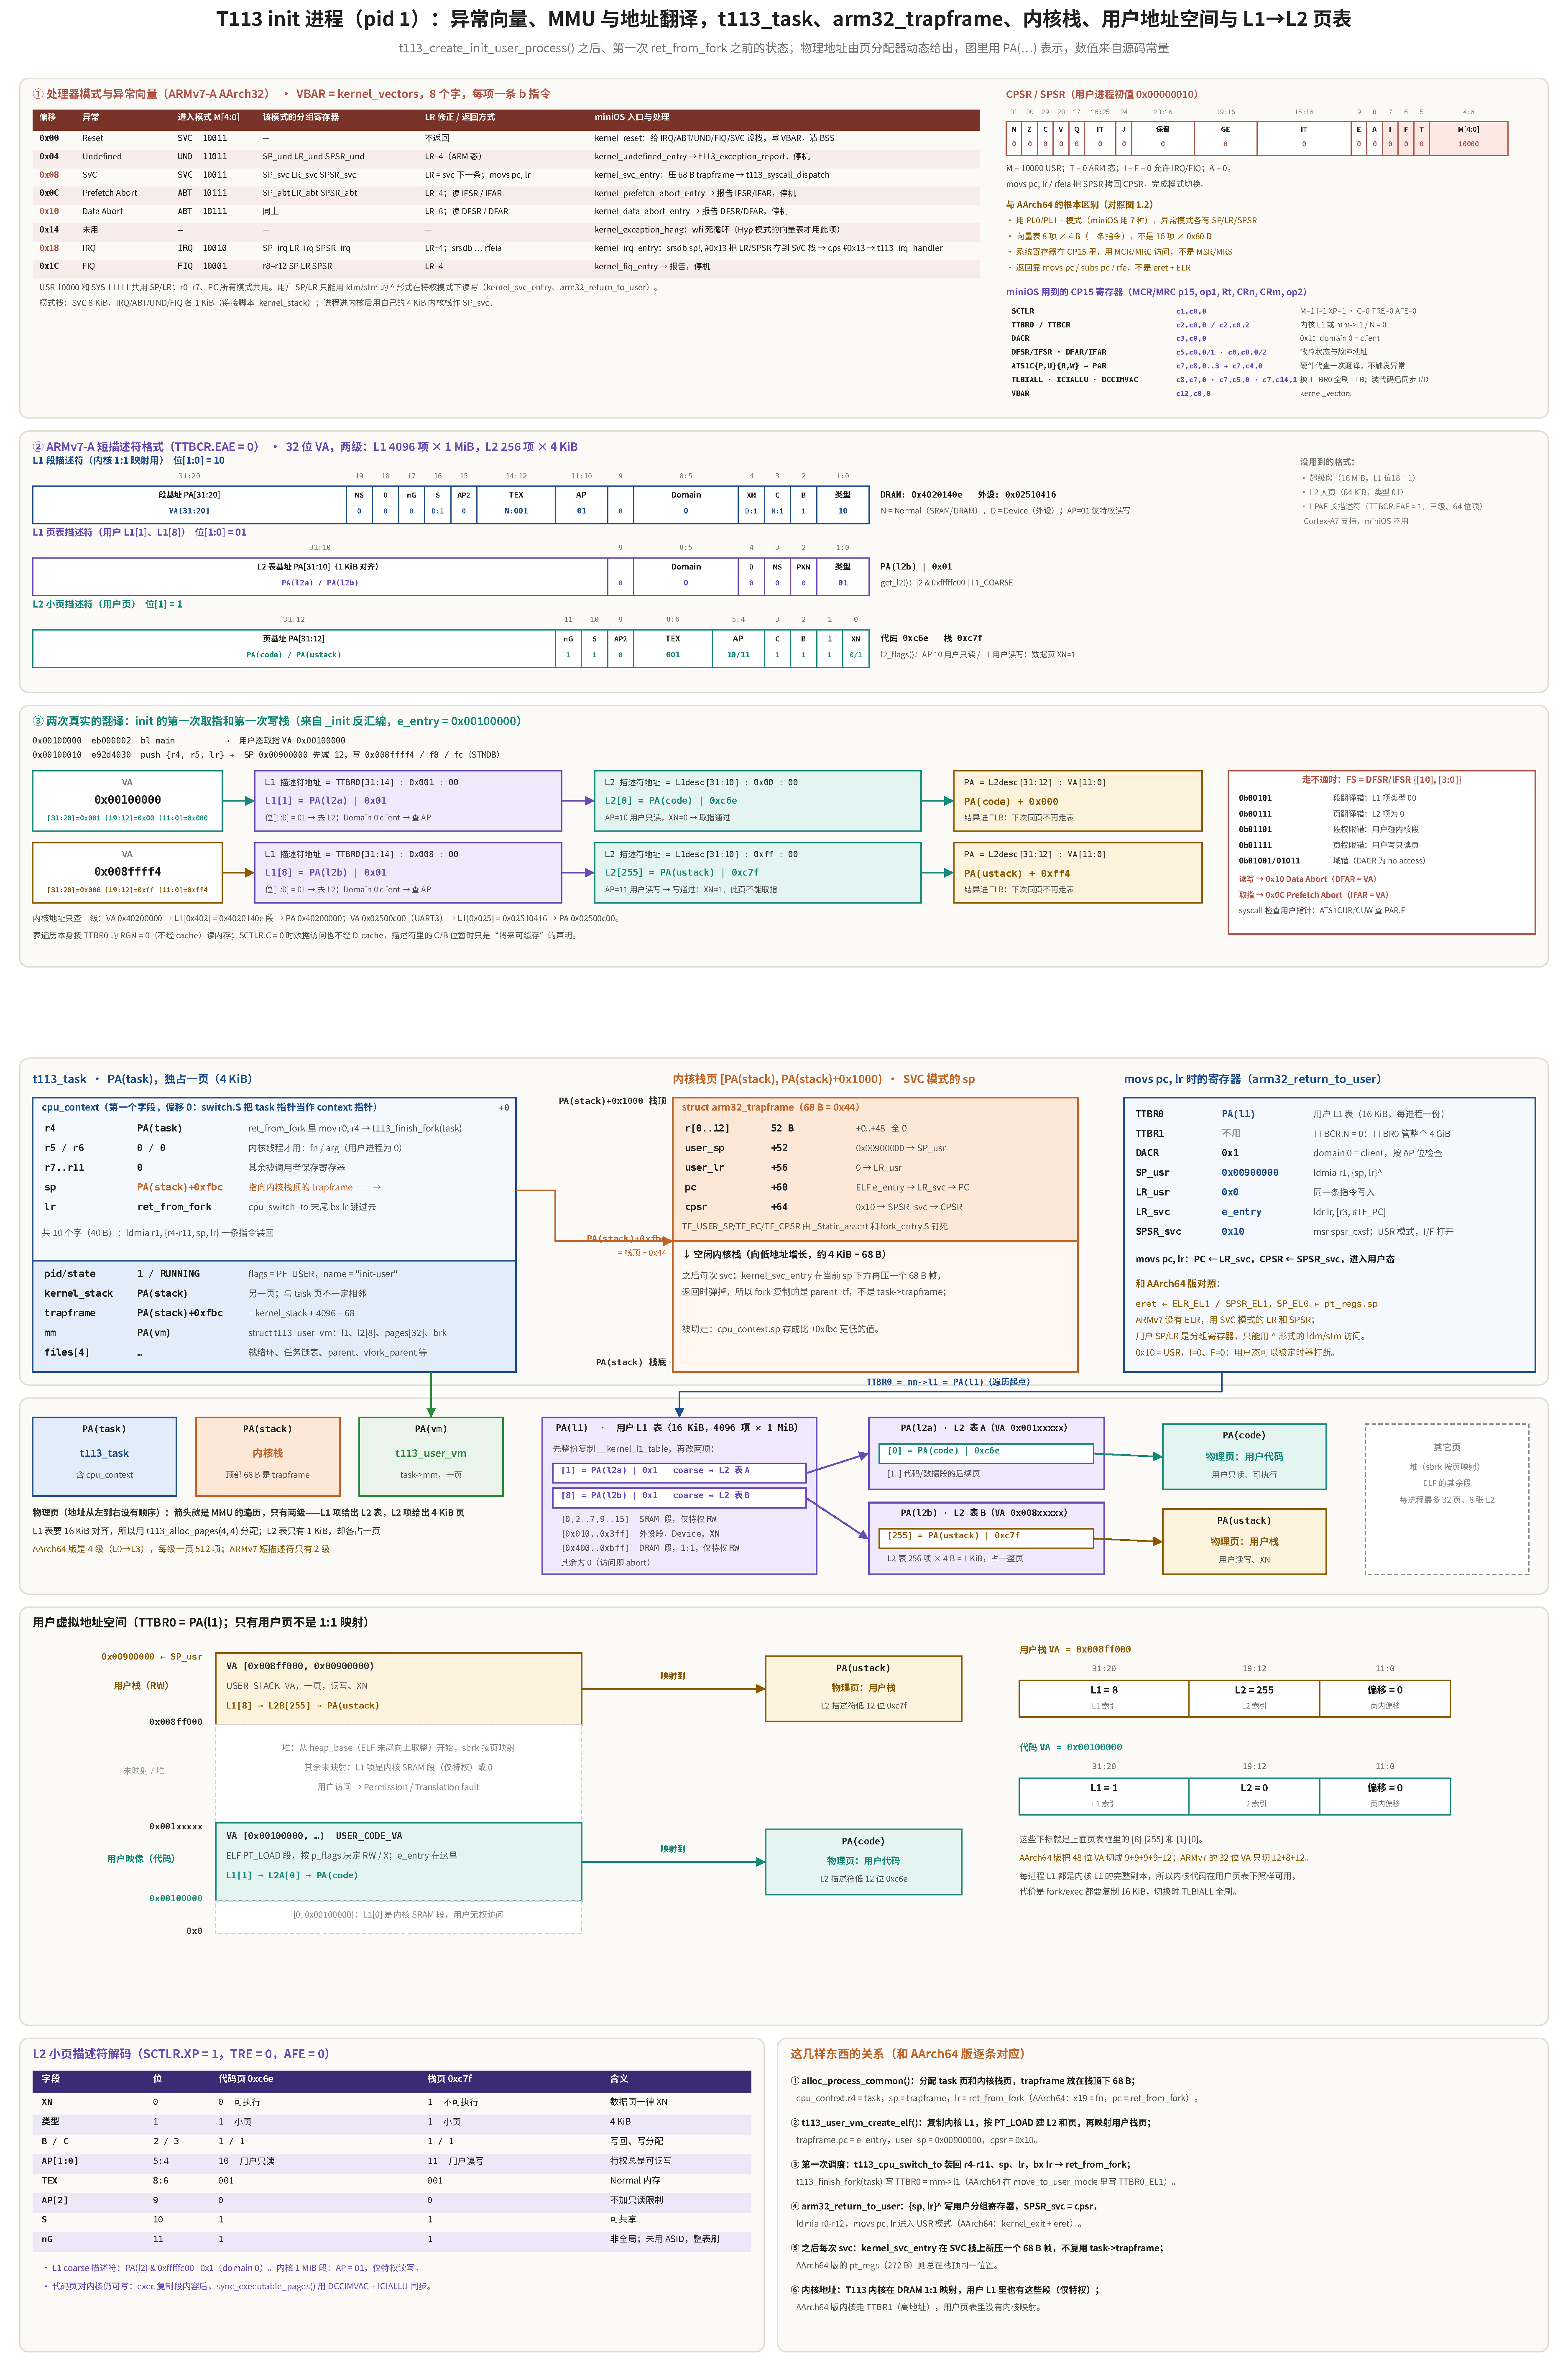
\includegraphics[width=\linewidth]{figures/t113-proc-vm-pid1.pdf}
  \caption{T113 init 进程：异常向量、MMU 与地址翻译，\code{t113\_task}、\code{arm32\_trapframe}、内核栈、用户地址空间与 L1→L2 页表}
  \label{fig:t113-proc-vm}
\end{figure}

\begin{figure}[p]
  \centering
  \includegraphics[width=\linewidth]{figures/bare-proc-vm-pid1_11.pdf}
  \caption{树莓派 AArch64 pid 1：\code{task\_struct}、\code{pt\_regs}、内核栈、用户地址空间与 L0→L3 页表}
  \label{fig:aarch64-proc-vm}
\end{figure}

两张图对照下来，差别集中在这几处：

\begin{table}[H]
\centering
\small
\begin{tabularx}{\linewidth}{>{\raggedright\arraybackslash}X>{\raggedright\arraybackslash}X>{\raggedright\arraybackslash}X}
\toprule
方面 & 树莓派 AArch64 & T113 ARMv7-A \\
\midrule
切换上下文 & x19–x29、fp、sp、pc（x19 = fn） & r4–r11、sp、lr（r4 = task，r5/r6 = 内核线程的 fn/arg） \\
用户寄存器帧 & \code{pt\_regs} 272 B，总在栈顶同一位置 & \code{arm32\_trapframe} 68 B，每次 svc 在当前 sp 下新压一个 \\
回到用户态 & \code{kernel\_exit} + \code{eret}，ELR\_EL1 / SPSR\_EL1 / SP\_EL0 & \code{ldmia \{sp, lr\}\textasciicircum{}} + \code{msr spsr} + \code{movs pc, lr} \\
页表 & 4 级（L0→L3），每级 512 项，48 位 VA & 2 级短描述符：L1 4096 项 × 1 MiB（16 KiB），L2 256 项 × 4 KiB \\
内核映射 & TTBR1\_EL1，高地址，用户页表里没有 & TTBCR.N = 0，每个用户 L1 都是内核 L1 的完整副本（段只允许特权访问） \\
用户布局 & 代码 0x400000，栈顶 0x8000000 & 代码 0x00100000，栈顶 0x00900000 \\
进入用户态时的状态寄存器 & SPSR = 0x3c0（EL0t，DAIF 全屏蔽） & CPSR = 0x10（USR，IRQ/FIQ 打开） \\
\bottomrule
\end{tabularx}
\end{table}

\subsubsection*{AArch32 的异常、MMU 与地址翻译}

\textbf{处理器模式和分组寄存器。} ARMv7-A 不用 AArch64 的 EL，而是用特权级 PL0/PL1（虚拟化扩展另有 PL2）加处理器模式。miniOS 用到其中 7 种：USR、SYS、SVC、IRQ、FIQ、ABT、UND；Cortex-A7 另有 MON（安全扩展）和 HYP（虚拟化扩展），miniOS 不用。模式号在 CPSR[4:0]。除 USR/SYS 共用一组外，每种异常模式都有自己的 SP、LR、SPSR（FIQ 还有自己的 r8–r12）。所以\code{kernel\_reset} 要依次 \code{cps} 进每种模式设栈（SVC 8 KiB，其余各 1 KiB）；用户态的 SP/LR 在特权模式下看不见，\code{kernel\_svc\_entry} 和 \code{arm32\_return\_to\_user}只能用 \code{stmia/ldmia \{sp, lr\}\textasciicircum{}} 这种带 \code{\textasciicircum{}} 的形式访问。

\textbf{异常向量。} \code{VBAR}（CP15 c12）指向 \code{kernel\_vectors}，表里是 8 条\code{b handler} 指令，每项 4 字节，按偏移 0x00 Reset、0x04 Undefined、0x08 SVC、0x0C Prefetch Abort、0x10 Data Abort、0x14 未用、0x18 IRQ、0x1C FIQ 排列。进入异常时硬件把返回地址放进该模式的 LR，旧 CPSR 放进 SPSR；LR 的偏移因异常而异（Undef/Prefetch/IRQ/FIQ 减 4，Data Abort 减 8，SVC 不用改）。返回也不是一条统一指令：SVC 用 \code{movs pc, lr}，IRQ 先用 \code{srsdb sp!, \#0x13} 把 LR\_irq 和SPSR\_irq 压到 SVC 栈，处理完再用 \code{rfeia sp!} 一次恢复 PC 和 CPSR。Undef、Abort、FIQ 在 miniOS 里只报告现场然后停机。

\textbf{CP15 与 MMU 配置。} 系统寄存器都在协处理器 CP15 里，用 \code{mcr/mrc p15, …}访问。\code{t113\_mmu\_init()} 写 TTBR0 = \code{\_\_kernel\_l1\_table}、TTBCR = 0（N = 0，TTBR0 覆盖整个 4 GiB，TTBR1 不参与）、DACR = 1（domain 0 为 client，按 AP位检查），再在 SCTLR 里打开 M、I、XP，清 TRE、AFE，并且暂不打开 C（D-cache）。内核 L1 全是 1 MiB 段，1:1 映射：0x000–0x00F MiB 是 SRAM（Normal），0x010–0x3FF MiB 是外设（Device、XN），0x400–0xBFF MiB 是 DRAM（Normal），都只允许特权访问（AP = 01）。

\textbf{短描述符和两级翻译。} 32 位 VA 拆成 [31:20] L1 索引、[19:12] L2 索引、[11:0] 页内偏移。

\begin{txtcode}
L1 描述符地址 = TTBR0[31:14] : VA[31:20] : 00
   位[1:0] = 10 → 段：PA = desc[31:20] : VA[19:0]            （内核，查一级就结束）
   位[1:0] = 01 → 页表：继续
L2 描述符地址 = L1desc[31:10] : VA[19:12] : 00
   位[1]   = 1  → 小页：PA = desc[31:12] : VA[11:0]
\end{txtcode}

每个用户 L1 都是内核 L1 的完整副本，只把 L1[1]（代码）和 L1[8]（栈）换成页表描述符。这一点与 Linux 在 ARM 短描述符下的做法相同：TTBCR.N = 0，每个进程的 pgd 都带一份内核映射。区别是 Linux 在同一页里还放了软件用的影子 PTE，miniOS 的 1 KiB L2 表则单独占一页。

\textbf{两次真实的翻译。} 从 \code{\_init} 的反汇编看，\code{e\_entry} = 0x00100000，第一条指令\code{bl main} 触发对 VA 0x00100000 的用户态取指：L1[1] → L2A[0] = PA(code) | 0xc6e，AP = 10（用户只读）、XN = 0，通过。\code{main} 的第一条指令 \code{push \{r4, r5, lr\}}在 SP = 0x00900000 时写 0x008ffff4–0x008fffff：L1[8] → L2B[255] = PA(ustack) | 0xc7f，AP = 11（用户读写），通过；同一页 XN = 1，不能取指。

\textbf{走不通时。} 翻译或权限检查失败，数据访问进 Data Abort（DFSR 给状态，DFAR给地址），取指进 Prefetch Abort（IFSR/IFAR）。FS 编码 0b00101/0b00111 是段/页翻译错，0b01101/0b01111 是段/页权限错。系统调用检查用户指针时，不让它真的出错，而是用 ATS1CUR/ATS1CUW（CP15 c7, c8）让硬件代查一次翻译，再看 PAR 的F 位（\code{t113\_mmu\_probe()}）。切换进程只换 TTBR0 并 TLBIALL 全刷，没有使用ASID（CONTEXTIDR）。



\subsection{子进程第一次运行：\code{ret\_from\_fork}}

\begin{txtcode}
t113_sched_tick() / t113_sched_yield()
+-- schedule_next()
    +-- 在就绪环里从 prev->ready_next 开始找 state == RUNNING
    |   +-- 一个都没有 → boot_context（kernel_boot 的 wfi 循环）
    +-- t113_current = next
    +-- switch_task_mm(next)            TTBR0 ← next->mm->l1 或内核 L1 表
    +-- t113_cpu_switch_to(prev, next)  switch.S
        +-- stmia r0, {r4-r11, sp, lr}  保存 prev
        +-- ldmia r1, {r4-r11, sp, lr}  装入 next：r4=task, sp=trapframe, lr=ret_from_fork
        +-- bx lr
            +-- ret_from_fork           fork_entry.S
                +-- t113_finish_fork(r4)
                |   +-- PF_KTHREAD → t113_switch_kernel_vm()
                |   +-- PF_USER    → t113_switch_user_vm(task->mm)
                +-- 内核线程：cpsie i; mov r0, r6; blx r5
                |   +-- fn(arg) 返回 → t113_task_exit()   state = IDLE, wfi
                +-- 用户进程：t113_task_trapframe(r4) → arm32_return_to_user(tf)
                    +-- ldmia {sp, lr}^        写 User 模式的 banked SP/LR
                    +-- lr  = tf->pc
                    +-- spsr = tf->cpsr        0x10 = User 模式，IRQ 打开
                    +-- ldmia r0-r12           r0 = 0
                    +-- movs pc, lr            CPSR ← SPSR，跳到 svc 的下一条
                        +-- 子进程在用户态从 fork()/vfork() 返回 0
\end{txtcode}

\code{r4/r5/r6} 是 miniOS 自己定的约定：它们是被调用者保存寄存器，\code{t113\_cpu\_switch\_to} 会原样恢复，所以可以用来把“任务指针、内核函数、参数”带到 \code{ret\_from\_fork}。AArch64 版本用的是 \code{x19/x20}，道理相同。

\subsection{vfork：父进程怎样等、怎样被唤醒}

\begin{txtcode}[basicstyle=\ttfamily\scriptsize]
 父进程 P                          调度器                      子进程 C
 vfork() - svc #0, r7 = 14 -→ t113_syscall_dispatch(tf)
   t113_vfork_user(tf)
     t113_kernel_clone(VM|VFORK)
       C.mm = P.mm（references = 2）
       C.vfork_parent = P
       P.state = WAITING
     t113_sched_yield() ------→ schedule_next()
                                P 不是 RUNNING，跳过
                                选中 C ----------------------→ ret_from_fork
                                                               用户态 vfork() 返回 0
                                                               exec("/bin/ls", argv)
                                                               +-- sys_exec()
                                                                   +-- 新建 vm，装入 ELF
                                                                   +-- C.mm = 新 vm
                                                                   +-- t113_vfork_complete(C)
                                                                   |   +-- P.state = RUNNING
                                                                   |   +-- C.vfork_parent = 0
                                                                   +-- 切 TTBR0 到新 vm
                                                                   +-- t113_user_vm_put(P 的 mm)
                                                                       references = 1
                                ...之后某次调度选中 P
 ←---------------------------- t113_sched_yield() 返回
 t113_vfork_user() 返回 C 的 pid
 用户态 vfork() 返回 C 的 pid
\end{txtcode}

\code{t113\_vfork\_complete()} 有两个调用点，对应 Linux 在 \code{mm\_release()} 里\code{complete(vfork\_done)} 的两种情况：

\begin{itemize}
  \item \code{sys\_exec()}（\code{src/kernel/syscall.c}）：子进程换上了自己的地址空间；
  \item \code{t113\_exit\_current()}（\code{sched/core.c}）：子进程没 exec 就退出了。
\end{itemize}

父进程用的是 \code{WAITING} 状态，不是忙等。\code{t113\_exit\_current()} 里，“父进程在WAITING 就改回 RUNNING”这条规则同时服务了 \code{wait()} 和 vfork。

\begin{note}
注意：vfork 的子进程在父进程的用户栈上运行。\code{user-t113/usys.S} 的 \code{\_\_sys\_vfork} 用 \code{push \{r7, lr\}} / \code{pop \{r7, pc\}}保存返回地址，\code{libc.c} 的 \code{vfork()} 又是 C 包装。子进程返回后再调用\code{exec()}，新的栈帧会落在同一片栈上，覆盖父进程还没弹出的返回地址。父进程恢复后从被改写的栈上返回，就会跳错地方。glibc 在 ARM 上用汇编写vfork，把返回地址留在寄存器里、不碰栈，原因就在这里。目前\code{user-t113/} 里还没有程序调用 \code{vfork()}；要用它，应先把包装改成不使用栈的汇编，或在子进程里直接内联 \code{svc}。
\end{note}

\subsection{地址空间：共享还是复制}

\begin{txtcode}[basicstyle=\ttfamily\scriptsize]
struct t113_user_vm（一页）
+-- references                      vfork 共享时为 2
+-- l1 --→ 16 KiB L1 表（4096 项，每项管 1 MiB）
|          +-- 内核区：创建时整表拷贝 __kernel_l1_table
|          +-- 用户区：指向 l2[]（最多 8 张 L2 粗页表）
+-- pages[32]  {va, pa, writable, executable}
|          代码 0x00100000 起，栈 0x008ff000–0x00900000，堆 [heap_base, brk)
+-- page_count / heap_base / brk

fork  : t113_user_vm_clone(src)
        +-- 新 vm 页 + 新 16 KiB L1（拷贝内核项）
        +-- 对 src->pages[i]：map_page(va, 同权限) + copy_bytes(4 KiB)
        +-- heap_base / brk 照抄
        +-- sync_executable_pages()       代码页逐行 DCCIMVAC，再 ICIALLU，保证取指看到新内容
vfork : child->mm = parent->mm; references++
exec  : 新建 vm，成功后 t113_user_vm_put(旧 vm)
wait  : 回收僵尸时 t113_user_vm_put(zombie->mm)
\end{txtcode}

T113 没有写时复制，fork 的代价正比于用户页数（最多 32 页，即 128 KiB 的memcpy）。这也是 vfork 存在的意义：shell 的“fork 后马上 exec”可以省掉这次拷贝。

\subsection{exit 与 wait}

\begin{txtcode}
t113_exit_current(status)                 T113_SYS_EXIT
+-- t113_vfork_complete(self)             没 exec 就退出的 vfork 子进程也要放行父进程
+-- 关闭 files[0..3]
+-- 子进程过继给 init_task                  与 xv6 reparent() 相同
|   +-- 有已是 ZOMBIE 的且 init 在 WAITING → 唤醒 init
+-- exit_status = status, state = ZOMBIE
+-- parent 在 WAITING → RUNNING
+-- t113_sched_yield()，不再返回

t113_wait_child(&status)                  T113_SYS_WAIT
+-- 循环
    +-- 扫 task_head 链表找 parent == current 的子进程
    +-- 有 ZOMBIE：摘链 → t113_user_vm_put(mm) → 释放 task/栈页 → 返回 pid
    +-- 一个子进程都没有 → -1
    +-- 否则 state = WAITING，yield，被 exit 唤醒后重扫
\end{txtcode}

\subsection{与 xv6 的进程创建对照}

xv6（这里对照的是 \code{xv6-aarch64/kernel/proc.c}）只有 \code{fork()}，没有 vfork 和clone，也没有内核线程。它的调用链：

\begin{txtcode}
sys_fork() → fork()                                  kernel/proc.c
+-- allocproc()
|   +-- 遍历 proc[NPROC] 找 UNUSED，持有 p->lock 返回
|   +-- pid = allocpid()
|   +-- trapframe = kstack + PGSIZE - sizeof(trapframe)   aarch64 移植放在内核栈顶
|   +-- pagetable = uvmcreate()
|   +-- context.x30 = forkret, context.sp = trapframe 处
+-- uvmcopy(p->pagetable, np->pagetable, p->sz)      逐页 kalloc + memmove，没有 COW
+-- np->sz = p->sz
+-- *(np->trapframe) = *(p->trapframe)
+-- np->trapframe->x0 = 0                            子进程返回 0
+-- ofile[i] = filedup(); cwd = idup()
+-- np->parent = p                                   持 wait_lock
+-- np->state = RUNNABLE

scheduler()                                          每个 CPU 一个调度循环
+-- swtch(&c->context, &p->context)
    +-- forkret()
        +-- release(&p->lock)                        scheduler 持锁切过来
        +-- 第一次：fsinit(ROOTDEV)                  文件系统初始化要能 sleep
        +-- usertrapret(tf) → eret 回 EL0
\end{txtcode}

\begin{table}[H]
\centering
\small
\begin{tabularx}{\linewidth}{l>{\raggedright\arraybackslash}X>{\raggedright\arraybackslash}X}
\toprule
方面 & xv6-aarch64 & T113 miniOS \\
\midrule
创建接口 & 只有 \code{fork()} & \code{t113\_kernel\_clone(flags)} 一个入口，派生 fork、vfork、内核线程 \\
进程表 & 静态 \code{proc[NPROC]}，每项一把 \code{p->lock} & 每个任务动态分配一页，\code{task\_head} 链表 + 就绪环，一把 \code{sched\_lock} \\
地址空间 & 4 级页表，\code{uvmcopy} 按 \code{p->sz} 逐页复制 & ARMv7 短描述符 L1/L2，\code{t113\_user\_vm\_clone} 按 \code{pages[]} 逐页复制 \\
共享地址空间 & 不支持 & \code{T113\_CLONE\_VM} + \code{references} 引用计数 \\
父进程等待 & 只有 \code{wait()}，用 sleep/wakeup 加通道 & \code{wait()} 和 vfork 都用 \code{WAITING} 状态，exit/exec 改回 \code{RUNNING} \\
第一次运行 & \code{forkret} → \code{usertrapret} & \code{ret\_from\_fork} → \code{t113\_finish\_fork} → \code{arm32\_return\_to\_user} \\
调度切换 & 进程 \ensuremath{\leftrightarrow} 每 CPU 的调度线程（两次 \code{swtch}） & 进程 \ensuremath{\leftrightarrow} 进程直接 \code{t113\_cpu\_switch\_to}，单核 \\
内核线程 & 无 & \code{T113\_CLONE\_KTHREAD}，\code{r5/r6} 带函数和参数 \\
返回值寄存器 & \code{trapframe->x0} & \code{trapframe->r[0]} \\
文件系统初始化 & 第一个进程的 \code{forkret} 里 \code{fsinit()} & \code{kernel\_boot()} 里在创建 init 之前挂好 \\
\bottomrule
\end{tabularx}
\end{table}

\subsection{与 Linux 的对照}

Linux 的 fork、vfork、clone、clone3 和 \code{kernel\_thread()} 最后都进\code{kernel\_clone(struct kernel\_clone\_args *)}：

\begin{txtcode}[basicstyle=\ttfamily\scriptsize]
fork()        → kernel_clone({ .exit_signal = SIGCHLD })
vfork()       → kernel_clone({ .flags = CLONE_VFORK | CLONE_VM, .exit_signal = SIGCHLD })
clone(flags...) → kernel_clone({ .flags = flags, .stack = newsp, ... })
kernel_thread → kernel_clone({ .flags = CLONE_VM | CLONE_UNTRACED, .fn = fn, .fn_arg = arg, .kthread = 1 })

kernel_clone()
+-- copy_process()          copy_mm / copy_files / copy_fs / copy_sighand / copy_thread
+-- CLONE_VFORK → p->vfork_done = &vfork（completion）
+-- wake_up_new_task(p)
+-- CLONE_VFORK → wait_for_vfork_done()   子进程 exec/exit 时 mm_release() → complete()
\end{txtcode}

T113 的做法是这条路径的缩小版：

\begin{itemize}
  \item \code{T113\_CLONE\_VM} 对应 \code{copy\_mm()} 里共享还是 \code{dup\_mm()}；
  \item \code{vfork\_parent} + \code{WAITING} 对应 \code{vfork\_done} completion；
  \item \code{t113\_vfork\_complete()} 对应 \code{mm\_release()} 里的 \code{complete\_vfork\_done()}；
  \item 文件描述符总是逐个加引用，相当于 Linux 不带 \code{CLONE\_FILES} 时的\code{dup\_fd()}；
  \item 没有线程，因为没有用户态 clone 系统调用，也不能给子进程另指用户栈。
\end{itemize}

\subsection{树莓派 AArch64 与 T113 ARMv7 的实现区别}

\begin{table}[H]
\centering
\small
\begin{tabularx}{\linewidth}{>{\raggedright\arraybackslash}X>{\raggedright\arraybackslash}X>{\raggedright\arraybackslash}X}
\toprule
方面 & 树莓派（前文） & T113 \\
\midrule
创建函数 & \code{copy\_process(clone\_flags, fn, arg, stack)}，\code{clone\_flags} 复用 \code{PF\_KTHREAD} & \code{t113\_kernel\_clone(flags, parent\_tf, name, fn, arg)}，策略标志与 \code{PF\_*} 分开 \\
首次运行寄存器 & \code{x19 = fn}、\code{x20 = arg}，\code{pc = ret\_from\_fork} & \code{r4 = task}、\code{r5 = fn}、\code{r6 = arg}，\code{lr = ret\_from\_fork} \\
用户上下文 & \code{pt\_regs}（x0–x30、sp、pc、pstate） & \code{arm32\_trapframe}（r0–r12、user\_sp、user\_lr、pc、cpsr，68 B） \\
进入内核 & \code{svc \#0}，异常级 EL0 → EL1，\code{x8} 是调用号 & \code{svc \#0}，User → SVC 模式，\code{r7} 是调用号 \\
回用户态 & \code{kernel\_exit} → \code{eret}（ELR/SPSR\_EL1） & \code{ldmia \{sp,lr\}\textasciicircum{}} + \code{movs pc, lr}（SPSR\_svc） \\
用户页表 & \code{TTBR0\_EL1}，4 KiB 粒度多级表 & \code{TTBR0}，16 KiB L1 + 1 KiB L2，内核项拷进每张 L1 \\
用户进程来源 & 内核把嵌入的镜像拷进去（\code{move\_to\_user\_mode}） & 从根文件系统读 ELF（\file{/init}、\code{exec}） \\
fork/vfork 系统调用 & 无 & 有，另有 wait/exit/exec/sbrk \\
\bottomrule
\end{tabularx}
\end{table}

\chapter{根文件系统与 devfs}
\label{chap:rootfs}
本章对应当前 miniOS 的实现，说明内核如何从 SD 卡找到并挂载根文件系统（xv6 血统的 minifs）、VFS 挂载表的形状、\file{/boot} 的 FAT32 交接（bootfs）、\file{/dev} 设备文件（devfs），以及用户态 \file{/init}、\file{/bin/sh}是如何从根文件系统里跑起来的。

\begin{note}
\textbf{更新}：\file{/boot} 已改为内核直接读写的 FAT32 文件系统（bio + fat32），挂载顺序也改成先 \file{/} 再 \file{/boot}，详见 第~\ref{chap:bootfat32} 章。本章的 bootfs 小节现在描述的是 FAT32 挂载失败时的后备路径。
\end{note}

当前已打通的链路：

\begin{itemize}
  \item SPL 读 SD 128 KiB 的 bootpack 装内核，再读 FAT32 分区把 XR829固件装进 DDR 并补写 bootpack 头（交接）；
  \item 内核 \code{kernel\_boot()} 依次挂载 \file{/}（minifs，MBR 第 2 分区按需读）、\file{/boot}（FAT32，失败时退回 bootfs）、\file{/dev}（devfs），任一最终失败即 PANIC；
  \item XR829 驱动从 \file{/boot/*.bin} 经 VFS 读固件（不再打进 bootpack）；
  \item 内核从 \file{/} 读出 \file{/init} 创建第一个用户进程；\code{init} fork+exec \file{/bin/sh}，shell 及 \code{ls/cat/echo/...} 都从 minifs 经 VFS 加载。
\end{itemize}

尚未实现：文件写入（minifs 只读）、minifs 日志区、devfs 作为用户态stdio 后端、\code{mount}/\code{umount} 系统调用、多个块设备。

\section{SD 卡布局}

\begin{table}[H]
\centering
\small
\begin{tabularx}{\linewidth}{l>{\raggedright\arraybackslash}X>{\raggedright\arraybackslash}X}
\toprule
区域 & 位置 & 内容 \\
\midrule
Boot0（SPL） & 8 KiB 偏移，512 B & miniBoot，SRAM 里跑，负责 DDR init + 装内核 \\
bootpack & 128 KiB 偏移 & 512 B header + kernel 镜像（见 \code{bootpack.h}） \\
MBR 分区 1 & FAT32 & \code{boot\_xr829.bin} / \code{fw\_xr829.bin} / \code{sdd\_xr829.bin}（macOS 挂载于 \file{/Volumes/bootfs}） \\
MBR 分区 2 & minifs 根文件系统 & \code{build-t113/minifs.img} 整镜像 dd 进去，≥ 32 MiB \\
\bottomrule
\end{tabularx}
\end{table}

分区 2 没有文件系统以外的含义：\code{rootdev.c} 只是取 MBR 第二个分区表项的 LBA/长度当块设备用。分区本身用任何分区工具建（类型 0x83 即可），FAT32 分区 1 是给 SPL 固件加载和人工换固件用的。

\begin{txtcode}
SD 8 KiB    +------------+
            | Boot0 SPL  |  读 128 KiB bootpack → 装内核
SD 128 KiB  +------------+
            | bootpack   |  header + kernel @0x40200000
分区 1      +------------+
            | FAT32      |  SPL 读固件 → DDR 0x40100000/0x40110000/0x40140000
分区 2      +------------+
            | minifs     |  内核 rootdev 按需读（块设备，非预载）
            +------------+
\end{txtcode}

\section{总调用链}

\begin{txtcode}[basicstyle=\ttfamily\scriptsize]
miniBoot SPL
+-- spl_main()
    +-- load_bootpack()
        +-- t113_sd_init()                    SMHC0 识别卡
        +-- 读 SD 128 KiB bootpack header     CRC32 校验
        +-- 逐条目读镜像到 load_addr + CRC32  kernel → 0x40200000
        +-- header 拷到 0x401ff000            内核侧查找入口
        +-- load_fat32_firmware()             FAT32 交接
            +-- fat32_mount()                 MBR 找 FAT32 分区, BPB 解析
            +-- fat32_load_root() × 3         boot/fw/sdd_xr829.bin → DDR
            +-- bootpack_slot()               补 3 个条目(offset=0 常驻), 重算 header CRC
        +-- 跳 0x40200000

miniOS kernel_main()                          boards/100ask_t113/platform_kernel.c
+-- t113_uart_init() / t113_mmu_init()
+-- t113_bootpack_dump()                      打印全部条目（含 SPL 交接的固件）
+-- kernel_boot()                             kernel/init/main.c
    +-- t113_page_alloc_init()                页分配器
    +-- t113_vfs_init()                       mount/super_block/inode/dentry/file 池清零
    +-- t113_minifs_mount_rootdev()           → /       失败 PANIC
    |   +-- t113_rootdev_init()               MBR 分区 2 解析
    |   |   +-- t113_sd_init()                SMHC0, 1-bit, 轮询
    |   |   +-- 读 LBA0, 验 0x55AA, 取表项 2  type/lba/sectors
    |   +-- 读 root_lba+2 扇区                块 1 = superblock
    |   +-- 验 magic 0x10203040, size×2 ≤ 分区扇区数 → t113_vfs_mount_fs("/")
    +-- t113_fat32_mount_vfs()                → /boot   读写 FAT32
    |   +-- 失败 → t113_bootfs_mount_vfs()    → /boot   SPL 交接视图，再失败 PANIC
    +-- t113_devfs_init()                     → /dev    失败 PANIC
    +-- net_init()                            CONFIG_NET
    +-- t113_driver_core_init()               平台/sdio 驱动绑定
    |   +-- uart probe → t113_chrdev_register(1/3, 0) + t113_devfs_create_chrdev("console"/"ttyS0")
    |   +-- xradio probe → need_image("/boot/*.bin")  经 VFS 读 FAT32 上的固件
    +-- t113_sched_init()
    +-- start_init_process()
    |   +-- t113_vfs_open("/init") → t113_vfs_read() → t113_create_init_user_process()
    +-- Timer0 + 开中断                       之后 idle: wfi

用户态
+-- /init (init.c)
    +-- fork() + exec("/bin/sh")              sys_exec: VFS 打开 → ELF → 新地址空间
    +-- wait() 孤儿回收, shell 退出后重启
\end{txtcode}

\file{/} 和 \file{/dev} 是硬依赖；\file{/boot} 先试 FAT32、再退回 bootfs，两者都失败才算失败。任何一个最终失败，\code{kernel\_boot()} 都打印 PANIC 并 \code{wfi} 死循环——没有根文件系统就没有用户态，无处可退。这对应 Linux “unable to mount root fs” 的 panic，只是 miniOS 连 initramfs 兜底都没有，也不需要：内核本身在 bootpack 里，卡上就是它的全部世界。挂载过程的图解见下一节。

\section{图解：内核怎样把根文件系统挂到 \file{/}}

\subsection{挂载结果}

先纠正一个容易混的点：devfs 挂在 \file{/dev}，不是 \file{/boot}。\file{/boot} 挂的是 SD 卡第一个分区上的 FAT32；只有 FAT32 挂载失败时，才退回到 bootfs（SPL 预加载镜像的只读视图）。启动完成后，整个命名空间是这样的：

\begin{txtcode}[basicstyle=\ttfamily\scriptsize]
SD 卡                                  VFS 挂载表 mounts[8]          命名空间
+--------------+
| MBR          |                       [0] "/"     → minifs_vfs_ops   /
| Boot0 / pack |                       [1] "/boot" → fat32_ops        +-- init
+--------------+  第 1 个 FAT32 分区     (失败时  → bootfs_ops)        +-- bin/ sh ls cat ...
| 分区 1 FAT32 | --------------------------------------------------→  +-- boot/                FAT32
+--------------+  MBR 表项 2                                          |   +-- boot_xr829.bin
| 分区 2 minifs| --------------------------------------------------→  |   +-- fw_xr829.bin
+--------------+                       [2] "/dev"  → devfs_ops        |   +-- sdd_xr829.bin
                                                                      |   +-- wifi.txt
内存：devfs nodes[16] -----------------------------------------------→ +-- dev/                 devfs
       （uart 驱动 probe 时注册）                                          +-- console
                                                                          +-- ttyS0
\end{txtcode}

\code{find\_mount()} 按最长前缀选后端。路径分隔符要求完整匹配，所以 \file{/bootx} 不会落到 \file{/boot}：

\begin{table}[H]
\centering
\small
\begin{tabularx}{\linewidth}{>{\raggedright\arraybackslash}X>{\raggedright\arraybackslash}X>{\raggedright\arraybackslash}X}
\toprule
路径 & 匹配的挂载点 & 后端 \\
\midrule
\file{/init} & \file{/} & minifs \\
\file{/bin/sh} & \file{/} & minifs \\
\file{/boot} & \file{/}、\file{/boot}，取 \file{/boot} & fat32（根目录） \\
\file{/boot/fw\_xr829.bin} & \file{/boot} & fat32 \\
\file{/bootx} & \file{/} & minifs（找不到就返回失败） \\
\file{/dev/console} & \file{/dev} & devfs \\
\bottomrule
\end{tabularx}
\end{table}

\subsection{启动时的挂载顺序}

\begin{txtcode}[basicstyle=\ttfamily\scriptsize]
SPL 跳到 0x40200000
+-- kernel_entry.S
    +-- kernel_main(dram_size)                     boards/100ask_t113/platform_kernel.c
        +-- t113_uart_init()                       早期串口
        +-- t113_mmu_init()                        内核 L1 表，打开 MMU
        +-- t113_bootpack_dump()
        +-- kernel_boot(pool_base, dram_end)        kernel/init/main.c，与板子无关的部分
            +-- t113_page_alloc_init()
            +-- t113_vfs_init()                    清空 mount/super_block/inode/dentry/file 五个池
            +-- t113_minifs_mount_rootdev()        (1) "/"   失败 → PANIC
            |   +-- t113_rootdev_init()
            |   |   +-- t113_sd_init()             SMHC0：CMD0/8/ACMD41/2/3/7，切到 12 MHz
            |   |   +-- t113_sd_read(0, 1, mbr)    验 55 AA
            |   |   +-- 表项 2：root_lba、root_sectors_count
            |   +-- t113_rootdev_read(2, 2, block_cache)     minifs 块 1 = 超级块
            |   +-- 验 magic 0x10203040，size × 2 ≤ 分区扇区数
            |   +-- t113_vfs_mount_fs("/", MINIFS_MAGIC, &fs_sb, &minifs_vfs_ops)
            +-- t113_fat32_mount_vfs()             (2) "/boot"
            |   +-- binit()                        建 bcache
            |   +-- bread(0)：MBR，找第一个 FAT32 类型的分区
            |   +-- bread(part_lba)：BPB 校验并算出布局
            |   +-- t113_vfs_mount_fs("/boot", 0x4d44, &fs, &fat32_ops)
            |       （先 lookup_path("/boot") 取 minifs 里的挂载点目录）
            |   失败 → t113_bootfs_mount_vfs()     (2') 退回 bootfs，再失败 → PANIC
            +-- t113_devfs_init()                  (3) "/dev"  失败 → PANIC
            +-- net_init()                         CONFIG_NET
            +-- t113_driver_core_init()            设备、驱动绑定
            |   +-- uart probe → t113_chrdev_register(1, 0, &console_fops)
            |   |                t113_chrdev_register(3, 0, &console_fops)
            |   |                t113_devfs_create_chrdev("console", 1, 0)
            |   |                t113_devfs_create_chrdev("ttyS0", 3, 0)
            |   +-- mmc_rescan_all() → xradio probe → need_image("/boot/*.bin")
            +-- t113_sched_init()
            +-- start_init_process()
            |   +-- t113_vfs_open("/init") → minifs
            |   +-- t113_vfs_read() 整个 ELF 读进临时页
            |   +-- t113_create_init_user_process()
            +-- 打开定时器和中断，进入 wfi 循环
\end{txtcode}

先挂 \file{/} 有一个具体原因：\code{t113\_rootdev\_init()} 负责 \code{t113\_sd\_init()}，也就是初始化 SMHC0 和 SD 卡；FAT32 和它共用这个控制器。驱动必须在\file{/boot}、\file{/dev} 都挂好之后才初始化，因为 XR829 的 probe 要从 \file{/boot} 读固件，UART 的 probe 要往 \file{/dev} 里注册节点。

\subsection{rootdev：分区到块设备}

minifs 的块是 1 KiB，SD 扇区是 512 B，\code{rootdev.c} 只做一次线性换算：

\begin{txtcode}
minifs 块号 b  --→  分区内扇区 2b, 2b+1  --→  整卡 LBA root_lba + 2b

t113_rootdev_read(sector, count, dst)
+-- 越界检查：sector + count ≤ root_sectors_count
+-- t113_sd_read(root_lba + sector, count, dst)
\end{txtcode}

它相当于 Linux 的分区块设备（\file{/dev/mmcblk0p2}），或 xv6 的 \code{ROOTDEV}加上 \code{virtio\_disk\_rw()}。区别是它不经过任何缓存，缓存放在 minifs 里（只缓存一块）。

\subsection{minifs 的磁盘布局和查找}

minifs 沿用 xv6 \code{mkfs} 的格式（\code{MINIFS\_MAGIC} 就是 xv6 的 \code{FSMAGIC} 0x10203040），布局和 xv6 一样：

\begin{txtcode}[basicstyle=\ttfamily\scriptsize]
块:  0       1        2 ... logstart+nlog-1   inodestart ...     bmapstart ...   数据块 ...
    +------+--------+----------------------+----------------+-------------+-------------+
    | boot | super  | log（minifs 不用）    | inode 块        | 空闲位图     | 文件/目录内容 |
    +------+--------+----------------------+----------------+-------------+-------------+
           magic size nblocks ninodes nlog logstart inodestart bmapstart

struct minifs_dinode（64 B，每块 16 个）
+-- type  1 = 目录，2 = 文件
+-- major minor nlink
+-- size
+-- addrs[12] 直接块 + addrs[12] 一个间接块（256 项）  → 最大 268 KiB

struct minifs_dirent（32 B）
+-- inum（u16）
+-- name[30]
\end{txtcode}

\code{exec("/bin/sh")} 在 minifs 里的查找：

\begin{txtcode}
t113_vfs_open("/bin/sh")
+-- minifs_vfs_lookup()
    +-- t113_minifs_open() → namei("/bin/sh")
        +-- current = ROOTINO (1)
        +-- "bin": directory_lookup(1, "bin")
        |   +-- read_inode(1)          块 inodestart + 1/16，取第 1 项
        |   +-- 逐个 32 B 目录项 inode_read() → 找到 inum = N
        +-- "sh":  directory_lookup(N, "sh") → inum = M
        +-- *inum = M；read_inode(M) 得到 size
sys_exec → t113_vfs_read(file, image, size)
+-- minifs_vfs_read() → t113_minifs_read(M, off, dst, n)
    +-- inode_read()
        +-- 每块：inode_block(inode, off / 1024)       直接块或间接块
                  block_address(b)                     命中 1 块缓存就直接用
                  +-- t113_rootdev_read(2b, 2, block_cache)
\end{txtcode}

和 xv6 的 \code{namex()} 相比，minifs 只读，所以不需要 inode 缓存、\code{ilock}、引用计数，也不需要日志。每次查找都从根目录开始，因为 T113 没有每进程的当前目录 inode（\code{getcwd} 返回的是固定的 \file{/}）。

\subsection{devfs：\file{/dev} 下的字符设备}

\begin{txtcode}[basicstyle=\ttfamily\scriptsize]
驱动 probe 时                           用户或内核 open("/dev/console")
t113_chrdev_register(1, 0,              t113_vfs_open("/dev/console", RDWR)
                     &console_fops)     +-- lookup_path：find_mount → "/dev" 挂载根 dentry
+-- chrdev_table[i] = { dev, ops }      |   +-- 分量 "console" → devfs_lookup("/dev/console")
t113_devfs_create_chrdev(               |       +-- devfs_basename() → "console"
   "console", 1, 0)                     |       +-- 遍历 nodes[]，id = MINIOS_MKDEV(1, 0)
+-- nodes[i] = { name, major, minor }   |           type = CHAR，private_data = &nodes[i]
                                        +-- devfs_open()：只接受 RDONLY / RDWR
                                        t113_vfs_write(f, "hi", 2)
                                        +-- devfs_write() → t113_chrdev_write(0x10000)
                                            +-- chrdev_table 按设备号 → console_fops.write()
                                                → UART3 发送
\end{txtcode}

devfs 的节点不在任何磁盘上，是驱动在内存里登记的表。这和 Linux 的 devtmpfs同一个思路：驱动注册设备时，内核自动在 \file{/dev} 下建节点。xv6 的做法不同：设备节点是磁盘上的 inode（\code{T\_DEVICE}，\code{mknod("console", CONSOLE, 0)} 由\code{init} 创建），\code{read/write} 时按 \code{ip->major} 查 \code{devsw[]} 分派。

用户态 \file{/init} 打开 \file{/dev/console}，再用 \code{dup()} 建立 fd 0/1/2；所有控制台I/O 都走 VFS → devfs → chrdev → UART，不再在系统调用层特判标准 fd。

\subsection{与 xv6、Linux 的挂载方式对照}

\begin{table}[H]
\centering
\small
\begin{tabularx}{\linewidth}{l>{\raggedright\arraybackslash}X>{\raggedright\arraybackslash}X>{\raggedright\arraybackslash}X}
\toprule
方面 & xv6 & Linux & T113 miniOS \\
\midrule
根文件系统从哪来 & 固定 \code{ROOTDEV}（virtio 盘，整盘是一个 fs） & \code{root=} 参数，\code{prepare\_namespace()} → \code{mount\_root()}，常先经 initramfs & MBR 第 2 分区，\code{t113\_minifs\_mount\_rootdev()} \\
何时挂载 & 第一个进程的 \code{forkret()} 里 \code{fsinit(ROOTDEV)}，因为读盘要 sleep & \code{kernel\_init} 线程里，在 exec \file{/sbin/init} 之前 & \code{kernel\_boot()} 里，在创建 init 之前；读盘是轮询，不用 sleep \\
有没有挂载表 & 没有，只有一个文件系统 & \code{struct mount} 树，\code{vfsmount} 挂在 dentry 上 & \code{vfs\_mount} 父子关系、mountpoint dentry，路径选择暂兼容最长前缀 \\
第二个文件系统 & 不支持 & 任意 & \file{/boot} FAT32、\file{/dev} devfs \\
设备文件 & 磁盘上的 \code{T\_DEVICE} inode + \code{devsw[major]} & devtmpfs，驱动注册时建节点 & devfs，驱动注册时登记 \\
挂载失败 & \code{panic("invalid file system")} & \code{VFS: Unable to mount root fs} panic & \code{kernel\_platform\_panic("cannot mount root filesystem")} \\
用户态 mount & 无 & \code{mount(2)} & 无 \\
\bottomrule
\end{tabularx}
\end{table}

\subsection{T113 实现上的区别}

\begin{itemize}
  \item 两个文件系统共用一个 SD 控制器（SMHC0）和一张卡。\code{rootdev.c} 不经\code{bio.c}；\code{fat32.c} 经 \code{bio.c}。两条路径都在 \code{t113\_sd\_read/write} 里的\code{sd\_lock} 汇合。
  \item VFS 已建立 \code{super\_block → dentry → inode → file} 对象链、引用计数和 inode/ dentry 缓存，并让子 mount 保存父 mount 与 mountpoint。minifs/FAT32/devfs仍通过兼容适配层接收累计的绝对路径；下一阶段可逐个改成真正的“父 inode + 单个分量” lookup，之后再完整处理 \code{.}、\code{..} 和跨 mount 回退。
  \item 卡上的 SPL、bootpack、两个分区由同一个 \code{make install} 写入；分区 2 必须足够放下 \code{minifs.img}（≥ 32 MiB）。
\end{itemize}

\section{VFS：super\_block、inode、dentry}

VFS 已改成 Linux 式的对象模型，完整说明见 第~\ref{chap:vfs} 章。这里只列和挂载、根文件系统直接相关的几点：

\begin{table}[H]
\centering
\small
\begin{tabularx}{\linewidth}{>{\raggedright\arraybackslash}X>{\raggedright\arraybackslash}X}
\toprule
miniOS & Linux \\
\midrule
\code{vfs\_mount} + \code{parent/mountpoint/mnt\_root} & \code{struct mount} / \code{vfsmount} \\
\code{super\_block} + \code{super\_operations}，\code{s\_backend} 指向旧后端 & \code{struct super\_block} \\
\code{dentry\_cache[128]}、\code{inode\_cache[128]} 与引用计数 & dcache / icache \\
\code{file} + \code{file\_operations} + \code{f\_pos\_lock} & \code{struct file} + \code{f\_count} \\
全局 \code{vfs\_lock} 一把互斥 & per-inode 锁 + RCU \\
\bottomrule
\end{tabularx}
\end{table}

\begin{itemize}
  \item \textbf{挂载}：\code{t113\_vfs\_mount\_fs(path, magic, fs\_info, ops)} 为每个文件系统建一个\code{super\_block}、一个根 inode 和一个根 dentry；不是 \file{/} 时还要先在父文件系统里 \code{lookup\_path(path)} 找到挂载点目录，所以 minifs 镜像里必须有 \file{/boot}、\file{/dev} 两个空目录（\code{mkfs\_minifs} 已经建好）。
  \item \textbf{选文件系统}：仍按最长前缀匹配（\file{/bootx} 不会落到 \file{/boot}），然后从那个挂载的根 dentry 开始逐级建 dentry。
  \item \textbf{后端接口没变}：\code{vfs\_backend\_ops.lookup} 仍收到累计的绝对路径，由 \code{vfs.c}里的 \code{backend\_iops/backend\_fops} 把 inode/file 操作转成后端调用。
  \item \textbf{身份}：minifs 的 inode 号、FAT32 的 \code{fat\_inode} 槽位地址、bootfs 的 DDR地址、devfs 的设备号成为 \code{inode->i\_ino}；同一文件多次打开共享一个 inode。
  \item 读写带 \code{f\_pos} 语义，但\textbf{没有 lseek}；标志支持 \code{VFS\_O\_RDONLY} / \code{VFS\_O\_RDWR}，外加 FAT32 用的 \code{VFS\_O\_CREATE} / \code{VFS\_O\_TRUNC}（值取自 xv6 \code{fcntl.h}）。\code{write} 由 devfs 和 FAT32 实现；minifs 和 bootfs 只读。
  \item \textbf{注意}：\code{minifs\_vfs\_lookup()} 目前只接受普通文件，逐级查找要它返回目录\file{/boot}、\file{/dev}、\file{/bin}，所以挂载 \file{/boot} 会失败，详见第~\ref{chap:vfs} 章。
\end{itemize}

\section{rootdev：MBR 分区 2 块设备}

\code{src/kernel/fs/rootdev.c} + \code{src/drivers/mmc/sunxi-sd.c}：

\begin{itemize}
  \item \code{sunxi-sd.c} 是 \textbf{SPL 和内核共用的一份源码}（\code{MINIOS\_KERNEL} 宏区分是否加 mutex）：SMHC0（\code{0x04020000}，PF0..PF5，1-bit 总线），CMD17 单块读、轮询、CPU 搬 FIFO。SPL 用它读 bootpack/FAT32，内核用它读根文件系统——同一张卡的同一个控制器。
  \item \code{t113\_rootdev\_init()}：读 LBA 0，验证 \code{0x55 0xAA} 签名，取 MBR偏移 \code{446+16} 的第二个分区表项：type（偏移 4）、起始 LBA（+8）、扇区数（+12），type 非零、LBA 非零、≥ 4 扇区才接受。
  \item \code{t113\_rootdev\_read(sector, count, dst)} 做范围检查后转\code{t113\_sd\_read(root\_lba + sector, ...)}。
\end{itemize}

\section{minifs：xv6 磁盘 ABI 的只读实现}

\code{tools/mkfs\_minifs.c}（主机侧）明确保留 xv6 mkfs 的磁盘格式，内核侧\code{src/kernel/fs/minifs.c} 是只读遍历实现。常量与 xv6 一致：

\begin{table}[H]
\centering
\small
\begin{tabularx}{\linewidth}{ll>{\raggedright\arraybackslash}X}
\toprule
常量 & 值 & 说明 \\
\midrule
\code{MINIFS\_BSIZE} & 1024 & 块大小（= 2 个 SD 扇区） \\
\code{MINIFS\_MAGIC} & 0x10203040 & xv6 \code{FSMAGIC} \\
\code{MINIFS\_ROOTINO} & 1 & 根目录 inode 号 \\
\code{MINIFS\_NDIRECT} & 12 & 直接块 \\
\code{MINIFS\_DIRSIZ} & 30 & 文件名上限 \\
\code{dinode} & 64 B & type/major/minor/nlink/size/addrs[13] \\
\code{dirent} & 32 B & u16 inum + name[30] \\
\bottomrule
\end{tabularx}
\end{table}

镜像布局（\code{FSSIZE=32768} 块 = 32 MiB，\code{NINODES=200}）：

\begin{txtcode}
块 0            空（xv6 惯例留空）
块 1            superblock
块 2..31        log 区（30 块，只读实现不使用，格式保留）
块 32..44       inode 区（200/16+1 = 13 块，每块 16 个 dinode）
块 45..49       位图（32768/8192+1 = 5 块）
块 50..         数据区（含目录内容）
\end{txtcode}

mkfs 产出的目录树（\code{miniOS/Makefile} 打包 \code{\_init \_sh \_ls \_echo \_pwd \_cat \_sleep \_uptime}）：

\begin{txtcode}
/                ino 1
+-- bin/         sh, ls, echo, pwd, cat, sleep, uptime
+-- dev/         空目录（minifs 里的占位；真设备在 devfs）
+-- init         与 /bin/init 同一 inode（nlink=2，硬链接）
\end{txtcode}

单文件上限 = 12 直接块 + 256 间接块 = 268 块 = 268 KiB；xv6 风格目录 inode 的 \code{size} 被取整到完整块（\code{round\_directory()}）。

\subsection{两种挂载方式}

\begin{table}[H]
\centering
\small
\begin{tabularx}{\linewidth}{>{\raggedright\arraybackslash}X>{\raggedright\arraybackslash}X>{\raggedright\arraybackslash}X}
\toprule
函数 & 数据来源 & 用途 \\
\midrule
\code{t113\_minifs\_mount\_vfs(image, bytes)} & DDR 里的镜像（\code{minifs\_image.o} 可 objcopy 进内核） & 备用路径；T113 当前未链接 \\
\code{t113\_minifs\_mount\_rootdev()} & MBR 分区 2，按需读块 & \textbf{当前使用} \\
\bottomrule
\end{tabularx}
\end{table}

块设备模式的关键是\textbf{单块缓存}：\code{block\_cache[1024]} + \code{cached\_block}只缓存最近一块。\code{block\_address(block)} 命中缓存直接返回指针，未命中则 \code{t113\_rootdev\_read(block*2, 2, cache)} 读两个扇区。这等于一个只有一项的 page cache——读 \file{/init} 这种顺序小文件足够，遍历目录时superblock（块 1）和 inode 区会反复换入换出，每读一个 dirent 的inode 都可能多一次 SD 读。xv6 的 buffer cache 是 30 块 LRU，这里刻意省掉了。

读路径（无 dcache、无 icache，每次 lookup 全程走磁盘）：

\begin{txtcode}
namei("/bin/sh")
+-- 逐分量 directory_lookup()
    +-- read_inode(dir_inum)                 块 = inodestart + inum/16
    +-- inode_read() 逐 dirent              inode_block(): 前 12 块直接, 之后查间接块
    +-- names_equal(disk_name, component)   名字 ≤30 字节, NUL/长度双判
\end{txtcode}

\section{bootfs：\file{/boot} 的 FAT32 交接}

\begin{note}
现在只是后备路径：正常情况下 \file{/boot} 由 \code{fat32.c} 挂载，见第~\ref{chap:bootfat32} 章。
\end{note}

背景：XR829 三个固件文件现在放在 FAT32 分区里（方便换固件不用重烧bootpack），但内核的 minifs 是只读小文件系统、rootdev 只认分区 2。解法是分工：\textbf{SPL 读 FAT32（fat32.c，MBR + BPB + 簇链，支持长文件名），内核只认 DDR 里已经就位的镜像}。

SPL 把固件装到 DDR 固定地址后，向 bootpack 头补写三个条目（\code{offset=0}表示"常驻镜像，非 pack 内偏移"），重算头 CRC：

\begin{table}[H]
\centering
\small
\begin{tabular}{llll}
\toprule
文件 & bootpack 条目 & DDR 地址 & 容量上限 \\
\midrule
boot\_xr829.bin & \code{boot\_xr829} & 0x40100000 & 64 KiB \\
fw\_xr829.bin & \code{fw\_xr829} & 0x40110000 & 192 KiB \\
sdd\_xr829.bin & \code{sdd\_xr829} & 0x40140000 & 64 KiB \\
\bottomrule
\end{tabular}
\end{table}

内核侧 \code{bootfs.c} 把这三条暴露成普通文件：

\begin{itemize}
  \item \code{lookup("/boot/fw\_xr829.bin")} → \code{t113\_bootpack\_find("fw\_xr829")}，\code{node.id = load\_addr}（物理地址当文件 id）；
  \item \code{read()} 就是 \code{memcpy}——数据已在 DDR，零拷贝语义。
\end{itemize}

XR829 驱动的 \code{need\_image()} 因此从硬编码 bootpack 查询改成了标准VFS 调用（\code{t113\_vfs\_open("/boot/fw\_xr829.bin")} → 读到页分配的缓冲），驱动不再依赖 bootloader 私有的地址常量。若 FAT32 分区缺失，SPL 回退使用 bootpack 内打包的固件（老路径仍保留）。

\section{devfs：\file{/dev} 设备文件}

\code{src/kernel/fs/devfs.c} 对应 Linux 早期的 devfs（现代等价物是devtmpfs）：

\begin{itemize}
  \item \code{t113\_devfs\_init()}：挂到 \file{/dev}，16 个节点槽，设备名 ≤ 30 字节且不含 \file{/}；
  \item 驱动 probe 时做两件事：\code{t113\_chrdev\_register(major, minor, ops)} 把设备号和驱动操作登记进 \code{chrdev.c} 的 \code{chrdev\_table[32]}（\code{ops} 至少要有read 或 write，设备号去重）；\code{t113\_devfs\_create\_chrdev(name, major, minor)}在 \file{/dev} 下建名字（名字去重）。这和 Linux 的 \code{register\_chrdev\_region} + \code{cdev\_add}、再由 devtmpfs 建节点是同一个分工；
  \item \code{lookup("/dev/console")}：\code{node.id = (major<<16)|minor}、\code{type = DEVFS\_T\_CHAR}、\code{private\_data} 指向节点；\file{/dev} 本身作为目录节点（type 1）返回，\code{readdir("/dev", i)} 枚举已注册设备；
  \item \code{read}/\code{write} 按 \code{node.id} 调 \code{t113\_chrdev\_read/write()}，再由\code{chrdev\_table} 找到驱动的 \code{ops}，\textbf{忽略 offset}——字符设备没有seek 语义，这和 Linux \code{struct file\_operations} 里 \code{.llseek = no\_llseek} 的约定一致。
\end{itemize}

当前唯一注册者是 UART 平台驱动（\code{uart.c} probe）：\code{console}（major 1, minor 0）和 \code{ttyS0}（major 3, minor 0），major 取值沿 Linux 惯例（1 = 内存/终端类，3 = 第一个 8250 串口）。注册时序有要求：\code{kernel\_boot()} 里的 \code{t113\_devfs\_init()} 必须早于驱动绑定 \code{t113\_driver\_core\_init()}，否则 probe 里的注册会失败。

\textbf{用户态 stdio}：\file{/init} 第一件事是 \code{open("/dev/console", O\_RDWR)} 得到fd 0，再 \code{dup(0)} 两次得到 fd 1、2；\code{syscall.c} 不再特判这三个 fd。shell继承的 stdin/stdout 就是这个 devfs 文件，三个 fd 共享同一个 \code{struct file}。另一个注册者是 \code{drivers/input/gpio\_keys.c} 的 \file{/dev/key0}。

\section{用户态视角：从 \file{/init} 到 shell}

系统调用到 VFS 的映射（\code{src/kernel/syscall.c}，每进程\code{files[T113\_MAX\_FDS=16]}，fd 0/1/2 由 \file{/init} 打开 \file{/dev/console} 建立）：

\begin{table}[H]
\centering
\small
\begin{tabularx}{\linewidth}{>{\raggedright\arraybackslash}X>{\raggedright\arraybackslash}X>{\raggedright\arraybackslash}X}
\toprule
系统调用 & 内核路径 & 备注 \\
\midrule
\code{open(path, flags)} & \code{sys\_open} → \code{t113\_vfs\_open} & 用户指针逐字节经 \code{user\_vm\_range\_mapped} 校验拷入 \\
\code{read(fd, buf, n)} & \code{t113\_vfs\_read} & 控制台经 devfs → chrdev → UART \\
\code{write(fd, buf, n)} & \code{t113\_vfs\_write} & 单次 ≤ 256 B \\
\code{dup(fd)} & \code{t113\_vfs\_file\_get} & 新 fd 共享同一个 \code{struct file} \\
\code{close(fd)} & \code{t113\_vfs\_close} & 引用计数归零才释放槽位 \\
\code{readdir(path, i)} & \code{t113\_vfs\_readdir} & \code{ls} 的实现基础 \\
\code{exec(path, argv)} & \code{sys\_exec} → \code{t113\_vfs\_open} + ELF 加载 & 镜像 ≤ 16 页（64 KiB） \\
\code{getcwd} & 常量 \code{"/"} & 尚无每进程 cwd，pwd 是假的 \\
\bottomrule
\end{tabularx}
\end{table}

内核加载 \file{/init} 本身（\code{kernel\_main} 尾部）就是一次普通 VFS 读：open → 按文件大小 \code{alloc\_pages} → read → \code{create\_init\_user\_process} → 释放临时页。\file{/init} 再 \code{fork()} + \code{exec("/bin/sh")}，shell 的每次命令执行又是一次 \code{exec} → VFS → minifs 读块。整条用户态生命线都吊在 rootdev 的 CMD17 上。

\section{与 Linux / xv6 的对照}

\begin{table}[H]
\centering
\small
\begin{tabularx}{\linewidth}{>{\raggedright\arraybackslash}X>{\raggedright\arraybackslash}X>{\raggedright\arraybackslash}X}
\toprule
miniOS & xv6 & Linux \\
\midrule
\code{vfs\_mount} 树 + 前缀匹配 & 无（只有一个 fs） & 挂载树 + namespace \\
\code{super\_block} / \code{inode} / \code{dentry} 对象池 & \code{itable} inode 缓存，无 dentry & super\_block、icache、dcache \\
\code{inode\_operations} / \code{file\_operations}（经 \code{vfs\_backend\_ops} 适配） & 无，直接调 fs 函数 & \code{inode\_operations} + \code{file\_operations} + \code{super\_operations} \\
\code{rootdev}（MBR 分区） & \code{ide} 驱动 & 块设备层 + 分区扫描（\code{read\_partition}） \\
minifs 只读 & xv6 fs（含 log 写入） & ext4 等 \\
单块缓存 & 30 块 buffer cache & page cache \\
\file{/boot} FAT32（失败时退回 bootfs） & — & \file{/boot} 分区 + firmware loader \\
devfs + \code{chrdev\_register} & mknod + \code{devsw[]} & devtmpfs + \code{device\_create}（+ udev 用户态改名） \\
\code{kernel\_main} 读 \file{/init} & 第一个进程硬编码在 initcode.S & initramfs 的 \file{/init} → exec \file{/sbin/init} \\
PANIC + \code{wfi} & \code{panic()} & \code{panic()} \\
\bottomrule
\end{tabularx}
\end{table}

\section{构建与烧写}

\begin{shcode}
make t113                    # 内核 + minifs.img（mkfs_minifs 打包 init/sh/ls/...）
make install T113_DISK=/dev/diskX
# 内部依次：
#   dd minios-t113.bin  @ 8 KiB    (Boot0)
#   dd bootpack.bin     @ 128 KiB  (kernel)
#   cp firmware/xr829/*.bin → /Volumes/bootfs   (FAT32, install-firmware)
#   dd minifs.img → /dev/diskXs2                (install-rootfs)
\end{shcode}

换固件只动 FAT32 分区；改用户程序（\code{user-t113/*.c}）只需重跑\code{install-rootfs}，内核和 bootpack 不用重烧。

\section{预期串口输出}

（LBA/大小以实际卡为准，下面是格式示例）

\begin{txtcode}[basicstyle=\ttfamily\scriptsize]
SPL: SDHC card ready
SPL: load kernel -> 0x40200000 bytes=0x?????? ok
SPL: FAT32 partition LBA=0x00002000
SPL: FAT32 load boot_xr829.bin bytes=0x888
SPL: FAT32 load fw_xr829.bin bytes=0x2aa20
SPL: FAT32 load sdd_xr829.bin bytes=0x2e8
...
bootpack: kernel @0x40200000 bytes=0x????????
bootpack: boot_xr829 @0x40100000 bytes=0x00000888
bootpack: fw_xr829 @0x40110000 bytes=0x0002aa20
bootpack: sdd_xr829 @0x40140000 bytes=0x000002e8
rootdev: MBR partition 2 type=0x83 lba=0x?????? sectors=0x??????
minifs: mounted block rootfs blocks=0x8000 inodes=0xc8
fat32: /boot mounted rw, partition lba=0x???????? clusters=0x???????? cluster-bytes=0x????????
...
init: starting shell on console
\end{txtcode}

\code{rootdev:}、\code{minifs:} 先出现，然后才是 \code{fat32:}：\code{kernel\_boot()} 先挂 \file{/}（它顺带初始化 SD 卡），再挂 \file{/boot}。FAT32 挂载失败时会多一行 \code{fat32: mount failed, using SPL handoff images}，接着是 \code{bootfs: FAT32 handoff mounted at /boot}。devfs 挂载没有打印，驱动绑定后 \code{platform\_dev\_info} 会打印 uart 绑定信息。

\chapter{/boot：从 bootpack 视图到可读写 FAT32}
\label{chap:bootfat32}

本章说明 \file{/boot} 的两代实现：改动前的 bootfs（bootpack 交接视图）和现在的 FAT32 文件系统（xv6 风格的 bio + fat32 分层），以及它们和 SPL、XR829 固件加载、tftp 的关系。根文件系统 minifs、VFS 挂载表、devfs 的整体结构见第~\ref{chap:rootfs} 章。

一句话总结：

\begin{itemize}
  \item \textbf{改动前}：读 FAT32 的是 SPL，内核里的 \file{/boot} 只是把 SPL 预先搬进 DDR 的三份固件包装成文件，只读、只认三个写死的路径、不能列目录。
  \item \textbf{改动后}：内核自己读写 SD 卡上的 FAT32 分区，\file{/boot} 是真正的文件系统，可以按文件名查找、列目录、创建和写入文件；tftp 下载的文件直接落盘到卡上。老的 bootfs 只在 FAT32 挂载失败时作为后备。
\end{itemize}

\section{改动前：bootfs 只是 bootpack 的视图}

\subsection{加载流程}

\begin{txtcode}[basicstyle=\ttfamily\scriptsize]
miniBoot SPL  load_bootpack()
+-- 读 SD 128 KiB bootpack，装 kernel → 0x40200000
+-- bootpack header 拷到 0x401ff000
+-- load_fat32_firmware()                 SPL 里的只读 FAT32 解析器
    +-- fat32_mount()                     MBR 找 FAT32 分区，解析 BPB
    +-- fat32_load_root() × 3             只在根目录按名字找，沿簇链读入 DDR
    |   +-- boot_xr829.bin → 0x40100000
    |   +-- fw_xr829.bin   → 0x40110000
    |   +-- sdd_xr829.bin  → 0x40140000
    +-- bootpack_slot()                   往 header 补 3 个条目（offset=0 表示常驻镜像），重算 CRC

miniOS 内核  bootfs.c（63 行）挂在 /boot
+-- lookup("/boot/fw_xr829.bin")
|   +-- 路径写死映射 → t113_bootpack_find("fw_xr829")
|       → node.id = load_addr（DDR 物理地址当文件 id）
+-- read() = 从 node.id + offset 处 memcpy
\end{txtcode}

\subsection{本质}

bootfs 本质上是\textbf{bootpack 解析器}，挂到 \file{/boot} 只是借用 VFS 的接口，让 XR829 驱动可以用 \code{t113\_vfs\_open("/boot/fw\_xr829.bin")} 拿固件，而不用知道 bootloader 私有的地址常量。它不是文件系统：

\begin{table}[H]
\centering
\begin{tabular}{llp{6.6cm}}
\toprule
能力 & bootfs & 原因 \\
\midrule
按文件名查找 & $\times$ & \code{entry\_name()} 只认三个硬编码路径，映射到 bootpack 条目名 \\
列目录（\code{ls /boot}） & $\times$ & \code{readdir = 0} \\
读任意文件 & $\times$ & 只有 SPL 预加载的三份固件 \\
写入 / 创建 & $\times$ & 没有 \code{write}、\code{create} \\
看到运行期卡上的变化 & $\times$ & 数据是启动时的 DDR 快照，内核从不访问 FAT32 分区 \\
\bottomrule
\end{tabular}
\end{table}

所以当时 tftp 之类``把文件存进 \file{/boot}''的功能无从实现。

\section{改动后：分层结构}

照 xv6 的 \file{bio.c} / \file{fs.c} 分层：

\begin{txtcode}
用户态  open(O_CREAT|O_TRUNC) / read / write / readdir / tftp
   |
VFS     src/kernel/fs/vfs.c        挂载表最长前缀匹配，/boot → fat32_ops
   |
fat32   src/kernel/fs/fat32.c      路径 → 目录项，文件偏移 → 簇链；inode 表
   |
bio     src/kernel/fs/bio.c        512 B 扇区缓存，24 块 LRU，写直达
   |
SD      src/drivers/mmc/sunxi-sd.c t113_sd_read / t113_sd_write（CMD17/CMD24，轮询）
\end{txtcode}

\subsection{挂载顺序}

\file{src/kernel/init/main.c} 的 \code{kernel\_boot()}：

\begin{ccode}
t113_vfs_init();
/* The root device initialises the SD card that /boot shares. */
if (t113_minifs_mount_rootdev() < 0)        /* 先挂 /，顺带初始化 SD 卡 */
    kernel_platform_panic("cannot mount root filesystem");
if (t113_fat32_mount_vfs() < 0) {           /* 再挂 /boot（FAT32 读写） */
    t113_uart_puts("fat32: mount failed, using SPL handoff images\n");
    if (t113_bootfs_mount_vfs() < 0)        /* 后备：老的 bootpack 视图 */
        kernel_platform_panic("cannot mount boot filesystem at /boot");
}
if (t113_devfs_init() < 0) ...
\end{ccode}

与之前相比，\file{/} 改为先挂（rootdev 里会做 \code{t113\_sd\_init()}，\file{/boot} 和 \file{/} 共用同一张卡、同一个 SMHC0 控制器）。两者都在调度器启动前完成，此时互斥锁实际不生效，SD 访问是串行的。

\section{bio：扇区缓存（\file{bio.c}）}

\begin{table}[H]
\centering
\begin{tabular}{ll}
\toprule
项 & 值 \\
\midrule
块大小 \code{BSIZE} & 512 B（= SD 扇区，块号就是卡上的绝对 LBA） \\
缓冲数 \code{NBUF} & 24 \\
替换策略 & 双向链表 LRU，\code{brelse} 后放到表头 \\
写策略 & \textbf{写直达}：\code{bwrite()} 立刻 \code{t113\_sd\_write()} \\
对齐 & \code{data[]} 4 字节对齐（SD 驱动用 CPU 搬 FIFO，按字访问） \\
\bottomrule
\end{tabular}
\end{table}

接口和 xv6 一致，多了一个 \code{bget\_blank()}：

\begin{table}[H]
\centering
\begin{tabular}{lp{9.2cm}}
\toprule
函数 & 作用 \\
\midrule
\code{bread(lba)} & 返回带引用的缓冲，未命中时从卡上读 \\
\code{bget\_blank(lba)} & 返回带引用的缓冲但\textbf{不读卡}，给``整块覆盖''的调用者（写满一个扇区、清零新簇）省一次读 \\
\code{bwrite(b)} & 写回卡上 \\
\code{brelse(b)} & 释放引用，缓冲留在缓存里 \\
\bottomrule
\end{tabular}
\end{table}

同一块的并发访问由上层串行化（fat32 每个操作都持有自己的锁），所以 bio 不像 xv6 那样给每个 buf 配 sleeplock。

因为是写直达，卡上的内容永远不比缓存旧，fat32 读大段数据时可以绕开缓存直接读卡（见下文``读路径''）。

\section{fat32（\file{fat32.c}）}

\subsection{挂载 \code{t113\_fat32\_mount\_vfs()}}

\begin{enumerate}
  \item \code{binit()}，\code{bread(0)} 读 MBR，验 \code{55 AA}，取\textbf{第一个}类型为 \code{0x0B/0x0C/0x1B/0x1C}（FAT32 CHS/LBA，含隐藏变体）的分区表项。
  \item 读分区首扇区（BPB），校验：\code{55 AA}、每扇区 512 字节、每簇扇区数非零、FAT 个数非零、根目录项数为 0（FAT32 特征）、每 FAT 扇区数和总扇区数非零。
  \item 算出布局：
\end{enumerate}

\begin{txtcode}
part_lba
+-- 保留区（含 BPB、FSInfo）         fat_lba  = part + BPB[14] 保留扇区数
+-- FAT × fats                       data_lba = fat_lba + fats × sectors_per_fat
+-- 数据区                           簇 n 的 LBA = data_lba + (n-2) × spc
\end{txtcode}

\begin{enumerate}
  \setcounter{enumi}{3}
  \item 簇数 = (总扇区 $-$ 元数据扇区) / spc，并用 FAT 表能描述的条目数封顶；根目录簇号必须合法。
  \item 挂到 \file{/boot}，打印 \code{fat32: /boot mounted rw, partition lba=… clusters=… cluster-bytes=…}。
\end{enumerate}

\subsection{内存中的 inode 表}

FAT32 没有 inode，文件的元数据（首簇、大小）存在目录项里。为了对齐 xv6 的 icache，fat32.c 维护一个 16 项的 \code{fat\_inode} 表：

\begin{ccode}
struct fat_inode {
    uint32_t ref;
    uint32_t dir;          /* 1 for a directory */
    uint32_t first;        /* first cluster, 0 for an empty file */
    uint32_t size;
    uint32_t ent_lba;      /* sector of the short entry, 0 for the root */
    uint32_t ent_off;      /* byte offset of that entry in the sector */
    uint32_t dirty;        /* first/size changed: rewrite the entry */
    uint32_t cur_index;    /* last cluster looked up: index in chain... */
    uint32_t cur_cluster;  /* ...and its number (0 = none) */
};
\end{ccode}

\begin{itemize}
  \item \textbf{身份} = 短目录项所在的 \code{(ent\_lba, ent\_off)}，同一个文件被打开两次会拿到同一个 inode（\code{iget} 按位置查找，引用计数 +1）。
  \item \code{vfs\_node.private\_data} 指向这个 inode，VFS 后续的 read/write/close 都通过它找到文件。
  \item \code{cur\_index / cur\_cluster} 缓存上一次查到的簇，顺序读写时沿簇链只往前走一步，不用每次从首簇开始数（簇链是单向链表）。
  \item \code{dirty}：写入导致首簇或大小变化时置位，\textbf{最后一次 close 时} \code{iupdate()} 把首簇（高 16 位 @20、低 16 位 @26）和大小（@28）写回目录项。
\end{itemize}

\subsection{路径解析}

\code{resolve(path)} 先用 \code{mount\_relative()} 去掉 \file{/boot} 前缀，然后逐个分量在目录簇链里用 \code{dir\_find()} 查找：

\begin{itemize}
  \item 目录遍历器 \code{dir\_next()} 同时拼接长文件名（LFN）片段，并用短名校验和（\code{short\_checksum()}）确认 LFN 和后面的短目录项属于同一个文件，否则退回用 8.3 短名。
  \item 名字比较不区分大小写；短名会按 NT 保留字节（byte 12）的大小写标志还原成小写。
  \item 支持任意层子目录；\code{..} 指向根目录时首簇为 0，按根目录簇处理。
  \item 根目录本身用 \code{lba = 0} 表示（它没有目录项）。
\end{itemize}

\subsection{读路径}

\begin{txtcode}
fat32_read(node, offset, dst, count)
+-- 循环
    +-- ibmap(ip, pos / 簇大小, alloc=0)   沿簇链找到所在簇
    +-- 扇区对齐 + 剩余 ≥ 512 + dst 4 字节对齐
    |   +-- t113_sd_read(lba, n, dst) 直接读进调用者缓冲（一次读完簇内剩余整扇区）
    +-- 否则 bread(lba) → copy 部分扇区 → brelse
\end{txtcode}

读大文件（固件、内核镜像）时绝大多数数据走直读，不占缓存也不多拷一次。

\subsection{写路径}

\begin{txtcode}
fat32_write(node, offset, src, count)
+-- offset > size → 拒绝（不支持稀疏文件）
+-- 循环
    +-- ibmap(ip, pos / 簇大小, alloc=1)   不够就 fat_alloc() 接到链尾
    +-- 写满一个扇区 → bget_blank()；否则 bread()（读改写）
    +-- copy → bwrite()（写直达）→ brelse
    +-- 文件变长 → ip->size 更新, dirty = 1
\end{txtcode}

\begin{itemize}
  \item \code{fat\_alloc(prev)}：从 \code{free\_hint} 开始线性扫 FAT 找值为 0 的簇，标成链尾 \code{0x0FFFFFFF}，再把 \code{prev} 指向它。
  \item \code{fat\_set()} 同时写\textbf{所有 FAT 副本}（通常 2 份），保持一致，Windows 和 macOS 的 fsck 不会报 FAT 不一致。
  \item 写 FAT 项只改低 28 位，保留高 4 位（规范要求）。
  \item \textbf{FSInfo}：第一次分配簇之前把 FSInfo 里的``空闲簇数 / 下一个空闲簇''标成未知（\code{0xFFFFFFFF}），让其它系统下次挂载时自己重新计算。这样内核就不需要维护精确的空闲计数。
\end{itemize}

\subsection{创建 \code{fat32\_create()}（\code{open} 带 \code{O\_CREAT}）}

\begin{enumerate}
  \item \code{resolve(path, parent=1)} 找到父目录和最后一个分量。
  \item 文件已存在就直接打开；否则 \code{create\_entry()}：
    \begin{itemize}
      \item 名字能直接放进 8.3（\code{fit\_short()}，大写字母、合法字符、基名 $\leq$ 8、扩展名 $\leq$ 3；全小写的名字用 NT 大小写标志记录）→ 只写一个短目录项；
      \item 否则生成别名 \code{NAME$\sim$N.EXT}（\code{make\_alias()}，N 从 1 递增直到不冲突），再写 $\lceil$长度/13$\rceil$ 个 LFN 项 + 1 个短目录项，LFN 项带短名校验和。
      \item \code{find\_slots()} 在父目录里找足够的连续空位（\code{0x00} / \code{0xE5}），不够就给目录追加一个清零的新簇。
      \item 创建日期写固定的 2026-01-01（\code{0x5c21}），没有 RTC。
    \end{itemize}
  \item 新文件首簇为 0、大小为 0，第一次写入时才分配簇。
\end{enumerate}

\subsection{截断 \code{fat32\_truncate()}（\code{open} 带 \code{O\_TRUNC}）}

顺序是\textbf{先改目录项、再释放簇链}：首簇和大小清零 → \code{iupdate()} 写回 → \code{fat\_free\_chain()}。如果中途掉电，最坏情况是留下一条无人引用的簇链（fsck 能回收），而不会出现目录项指向已经释放的簇。

\subsection{列目录 \code{fat32\_readdir()}}

跳过隐藏项、卷标、\code{.} 和 \code{..}；类型取值和 minifs 一致（1 = 目录，2 = 文件），所以现有的 \code{ls} 不用改。\code{vfs\_dirent.name} 只有 31 字节，超过 30 个字符的长文件名在 \code{ls} 里会被截断显示（打开文件时用完整名字没问题）。

\subsection{不支持}

\code{mkdir}、\code{unlink}、\code{rename}、时间戳更新、稀疏文件、多分区（只认 MBR 里第一个 FAT32 分区）、FAT12/16、exFAT。

\section{VFS 的配套改动}

\file{include/fs/vfs.h}：

\begin{ccode}
#define VFS_O_ACCMODE 3u
#define VFS_O_CREATE 0x200u      /* xv6 fcntl.h values */
#define VFS_O_TRUNC  0x400u

struct vfs_backend_ops {
    ...
    /* Optional: create an empty regular file (O_CREATE). */
    int (*create)(const char *path, struct vfs_node *node);
    /* Optional: discard a file's contents (O_TRUNC). */
    int (*truncate)(struct vfs_node *node);
    /* Optional: the last reference to an open node is gone. */
    void (*close)(struct vfs_node *node);
};
\end{ccode}

\code{t113\_vfs\_open()} 的流程：

\begin{txtcode}
find_mount(path)                    最长前缀匹配
+-- lookup(path) 失败
|   +-- 带 O_CREATE 且后端有 create → create(path)
+-- 带 O_TRUNC（必须是 O_RDWR）→ truncate(node)
+-- 分配 open_files 槽位
t113_vfs_write()   成功后更新 file->node.size
t113_vfs_close()   引用计数归零 → ops->close(node)   fat32 在这里写回目录项
\end{txtcode}

三个新回调都是可选的：minifs、devfs、bootfs 不实现它们，行为不变（对它们带 \code{O\_CREATE} 会失败）。

用户态：\file{fcntl.h} 增加 \code{O\_CREATE} / \code{O\_CREAT}（0x200）和 \code{O\_TRUNC}（0x400），\code{sys\_open} 接受这两个标志。

\section{谁在用 \file{/boot}}

\subsection{XR829 固件}

驱动代码没有改：\code{need\_image()}（现在在 \file{xradio/fwio.c}）一直是

\begin{ccode}
struct vfs_file *file = t113_vfs_open(
    "/boot/fw_xr829.bin", VFS_O_RDONLY);
\end{ccode}

变的是 VFS 下面的后端。现在这个调用由 fat32 处理：在 FAT32 根目录里按名字查找，沿簇链从卡上读出。也就是说固件加载现在走的是真正的文件系统查找；只有 FAT32 挂载失败时才会退回 bootfs 的 DDR 视图。

\textbf{注}：SPL 里的 \code{load\_fat32\_firmware()} 仍然会把三份固件预读进 DDR，内核正常路径已经不依赖它，只给 bootfs 后备路径用。上板确认 FAT32 稳定后可以删掉这段，启动会快一点。

\subsection{tftp}

\file{src/net/tftp/tftp\_udp.c} 的 \code{tftp\_get()}：先把整个文件收进内存（最多 8 MiB），传输完成后才 \code{t113\_vfs\_open(local, O\_RDWR | O\_CREATE | O\_TRUNC)} 写入，关闭后再重新打开读回、比对 CRC32。传输中断不会在 \file{/boot} 留下写了一半的文件。用户命令 \code{tftp <服务器IP> <远端文件> [本地路径]}，本地路径默认 \file{/boot/<文件名>}。

\subsection{WiFi 配置}

supplicant（\file{src/net/wpa/supplicant.c} 的 \code{wpa\_supplicant\_connect()}）从 \file{/boot/wifi.txt} 读 \code{ssid=}、\code{psk=}（以及可选的 \code{ip=}、\code{netmask=}、\code{gateway=}）。密码只放在 FAT32 分区上，不进源码；仓库里对应的 \file{rpi\_bm/firmware/wifi.txt} 被 \code{.gitignore} 忽略。

\subsection{SPL 从 FAT32 加载内核}

miniBoot \file{spl.c} 新增 \code{load\_fat32\_kernel()}：SD 初始化后先在 FAT32 根目录找 \code{kernel\_minios.img}（最大 8 MiB），读到 \code{0x40200000}，打印大小和 CRC32；找到了就跳过 bootpack 里的 kernel 条目，找不到就按原来的 bootpack 流程走。配合 tftp，可以在板子上直接更新内核：

\begin{shcode}
tftp 192.168.0.100                        # 写入 /boot/kernel_minios.img
# 重启后 SPL 加载新内核
\end{shcode}

想回到 bootpack 里的内核，删掉 FAT32 分区上的 \code{kernel\_minios.img} 即可。

\section{FAT32 图解（参照 xv6 book 第 8 章）}

xv6 book 讲文件系统时，先给一张分层图，再给磁盘布局，然后逐层讲buffer cache、inode、目录、路径名，最后串起 \code{open/read/write}。本节按同样的顺序讲 miniOS 的 FAT32，每一层都和 xv6 的对应层并排比较。

\subsection{分层}

\begin{txtcode}
        xv6 文件系统（7 层）                     miniOS /boot（T113）
 +-------------------------------+      +--------------------------------------+
 | 文件描述符  file.c sysfile.c  |      | task->files[4] → struct vfs_file     | vfs.c
 +-------------------------------+      +--------------------------------------+
 | 路径名      namei / namex     |      | find_mount() 选后端（最长前缀）       | vfs.c
 +-------------------------------+      | resolve() 逐级 dir_find()            | fat32.c
 | 目录        dirlookup/dirlink |      +--------------------------------------+
 +-------------------------------+      | 目录项 32 B 短名 + LFN 长名           | fat32.c
 | inode       iget/ilock/bmap   |      | fat_inode（内存）+ ibmap() 走簇链     | fat32.c
 +-------------------------------+      +--------------------------------------+
 | 日志        begin_op/end_op   |      | （无日志：直写 + 写入顺序约定）        |
 +-------------------------------+      +--------------------------------------+
 | buffer cache  bread/bwrite    |      | bio.c  24 个 512 B 扇区缓冲，LRU      | bio.c
 +-------------------------------+      +--------------------------------------+
 | 磁盘        virtio_disk.c     |      | t113_sd_read/write  SMHC0 CMD17/CMD24 | sunxi-sd.c
 +-------------------------------+      +--------------------------------------+
\end{txtcode}

xv6 的 inode 层同时负责“文件数据在哪些块”（\code{addrs[]} 加间接块）和“文件元数据存在哪”（磁盘 inode 区）。FAT32 把这两件事拆开了：

\begin{itemize}
  \item 数据块的位置记在 FAT 表里，一簇接一簇连成链表；
  \item 文件大小和首簇号记在父目录的 32 字节目录项里。
\end{itemize}

所以 miniOS 的 \code{fat\_inode} 只是内存里的一个句柄，记住“我的目录项在磁盘哪个位置”，关闭文件时把首簇和大小写回去。

\subsection{磁盘布局}

整张卡和 FAT32 分区内部：

\begin{txtcode}
整张 SD 卡（512 B 扇区，LBA = 扇区号）
LBA 0          MBR：446 B 引导码 | 4 × 16 B 分区表 | 55 AA
               表项 1  type 0x0b/0x0c   → FAT32  → 挂到 /boot
               表项 2  type 0x83        → minifs → 挂到 /
LBA 16         Boot0 SPL（8 KiB 处）
LBA 256        bootpack（128 KiB 处）
part_lba       FAT32 分区开始 -------------+
                                           v
part_lba   +---------------------------------+ +
           | 扇区 0  引导扇区（BPB）          | |
           | 扇区 1  FSInfo                  | | 保留区：BPB_RsvdSecCnt 个扇区
           | 扇区 6  备份引导扇区             | | （常见 32）
           | ...                              | |
fat_lba    +---------------------------------+ + = part_lba + RsvdSecCnt
           | FAT #1                          |   sectors_per_fat 个扇区
           | 每个簇一项，4 字节，低 28 位有效 |   一个扇区放 128 项
           +---------------------------------+
           | FAT #2（镜像）                   |   fat_set() 两份都写
data_lba   +---------------------------------+ = fat_lba + fats × sectors_per_fat
           | 簇 2   根目录通常从这里开始       |   cluster_lba(c) = data_lba + (c - 2) × spc
           | 簇 3                            |
           | ...                              |
           | 簇 clusters+1                   |
           +---------------------------------+
\end{txtcode}

xv6 的 \code{mkfs} 布局是连续的几段，块号由超级块给出：

\begin{txtcode}
xv6 (BSIZE = 1024)
[ 0 boot | 1 super | 2.. log | inodestart.. inode 块 | bmapstart.. 位图 | 数据块 ... ]
\end{txtcode}

两者对照：

\begin{table}[H]
\centering
\small
\begin{tabularx}{\linewidth}{>{\raggedright\arraybackslash}X>{\raggedright\arraybackslash}X>{\raggedright\arraybackslash}X}
\toprule
xv6 & FAT32 & miniOS 里在哪 \\
\midrule
超级块 \code{struct superblock} & 引导扇区里的 BPB & \code{t113\_fat32\_mount\_vfs()} 解析到全局 \code{fs} \\
空闲块位图 & FAT 表项为 0 表示空闲 & \code{fat\_alloc()} 从 \code{free\_hint} 线性扫描 \\
磁盘 inode 区 & 没有，元数据在目录项里 & 目录项的 \code{ent\_lba/ent\_off} \\
\code{addrs[12]} + 1 个间接块 & FAT 链表，长度不限 & \code{ibmap()} \\
日志区 & 没有 & 写入顺序约定（见后文） \\
\bottomrule
\end{tabularx}
\end{table}

\code{t113\_fat32\_mount\_vfs()} 用到的 BPB 字段：

\begin{table}[H]
\centering
\small
\begin{tabularx}{\linewidth}{lll>{\raggedright\arraybackslash}X}
\toprule
偏移 & 长度 & 字段 & 校验 / 用途 \\
\midrule
11 & 2 & BytsPerSec & 必须等于 512（\code{BSIZE}） \\
13 & 1 & SecPerClus & \code{fs.spc}，非 0 \\
14 & 2 & RsvdSecCnt & \code{fat\_lba = part\_lba + RsvdSecCnt} \\
16 & 1 & NumFATs & \code{fs.fats}，非 0 \\
17 & 2 & RootEntCnt & 必须为 0，这是 FAT32 的标志 \\
32 & 4 & TotSec32 & 算数据簇数 \code{clusters} \\
36 & 4 & FATSz32 & \code{sectors\_per\_fat} \\
44 & 4 & RootClus & \code{root\_cluster}，必须是合法簇号 \\
48 & 2 & FSInfo & FSInfo 扇区号，0 表示没有 \\
510 & 2 & 签名 & 55 AA \\
\bottomrule
\end{tabularx}
\end{table}

簇数还会再被 FAT 表的容量截一次：\code{clusters ≤ sectors\_per\_fat × 128 - 2}。有些格式化工具算出来的 FAT 偏小，截一下能防止 \code{fat\_get()} 越过 FAT 表。

\subsection{FAT 表与簇链}

FAT 表就是一个大数组，下标是簇号，值是“下一个簇号”：

\begin{txtcode}
目录项：name = "fw_xr829.bin"  first = 5  size = 174624

FAT[]  下标:  2     3     4     5     6     7     8     9     10    11
       值:   EOC   EOC   0     6     7     9     0     10    EOC   0
                         空闲  |     |     |     空闲  |     |     空闲
                               +-→ 6 +-→ 7 +---------→ 9 +-→ 10 → EOC

文件第 k 个簇 = 从 first 出发沿链走 k 步
偏移 off 所在的簇序号 = off / (spc × 512)
扇区 = cluster_lba(簇号) + (off % 簇字节) / 512
\end{txtcode}

（簇号只是示意。）表项取值：

\begin{table}[H]
\centering
\small
\begin{tabularx}{\linewidth}{l>{\raggedright\arraybackslash}X}
\toprule
值（低 28 位） & 含义 \\
\midrule
\code{0} & 空闲 \\
\code{2 … clusters+1} & 下一个簇 \\
\code{≥ 0x0ffffff8} & 链尾 EOC，miniOS 写 \code{0x0fffffff} \\
\bottomrule
\end{tabularx}
\end{table}

\code{ibmap(ip, index, alloc)} 把“文件第 index 个簇”翻译成簇号，相当于 xv6 的\code{bmap()}。差别在于：xv6 用下标直接查 \code{addrs[]}，O(1)；FAT 要从头走链，O(n)。miniOS 在 \code{fat\_inode} 里放了一个游标 \code{cur\_index/cur\_cluster}，顺序读写时从上一次的位置接着走，所以整文件顺序读还是 O(n) 而不是 O(n²)：

\begin{txtcode}
ibmap(ip, index, alloc)
+-- ip->first == 0（空文件）
|   +-- alloc ? first = fat_alloc(0) : 返回 0
+-- 起点：cur_index ≤ index 时从游标出发，否则从 first 出发
+-- while i < index:
|   +-- next = fat_get(c)               bread(FAT 扇区)，取 4 字节
|   +-- next 不是合法簇
|   |   +-- 是 EOC 且 alloc → next = fat_alloc(c)   扩链
|   |   +-- 否则返回 0（越过文件末尾）
|   +-- c = next, i++
+-- 更新游标，返回 c

fat_alloc(prev)
+-- fsinfo_invalidate()                 第一次分配时把 FSInfo 计数写成“未知”
+-- 从 free_hint 起环形扫描 FAT，找值为 0 的项
+-- fat_set(c, EOC)                     所有 FAT 副本
+-- prev ? fat_set(prev, c)             挂到链尾
+-- free_hint = c + 1
\end{txtcode}

\subsection{目录项}

FAT32 的目录也是文件，内容是一串 32 字节目录项。一个 512 B 扇区放 16 项，一个簇放 \code{spc × 16} 项。短目录项（8.3）的格式：

\begin{txtcode}
偏移  长度  字段
 0     8   主名，空格填充      e[0] = 0x00 目录结束；0xE5 已删除；0x05 表示首字符是 0xE5
 8     3   扩展名
11     1   属性   0x01 只读 0x02 隐藏 0x04 系统 0x08 卷标 0x10 目录 0x20 归档；0x0F = LFN
12     1   NT 保留  bit3 主名全小写，bit4 扩展名全小写
13     1   创建时间（10 ms）
14     2   创建时间
16     2   创建日期              miniOS 新建文件写 2026-01-01
18     2   访问日期
20     2   首簇号高 16 位   +
22     2   修改时间         |
24     2   修改日期         |
26     2   首簇号低 16 位   + first = (hi << 16) | lo
28     4   文件大小（目录为 0）
\end{txtcode}

长文件名（LFN）放在短目录项前面，每项 13 个 UTF-16 字符，按逆序存放：

\begin{txtcode}
磁盘顺序 →
+---------------+---------------+------------------------+
| LFN  0x42     | LFN  0x01     | 短项 "MINIOS~1BIN"     |
| 字符 14..17   | 字符 1..13    | attr 0x20 first size   |
| attr 0x0F     | attr 0x0F     |                        |
| chksum = S    | chksum = S    | S = short_checksum(名) |
+---------------+---------------+------------------------+
  0x40 标记“最后一片”（也就是磁盘上第一项）

LFN 项内 13 个字符的字节位置：lfn_pos[] = {1,3,5,7,9, 14,16,18,20,22,24, 28,30}
校验和：sum = ((sum & 1) << 7) + (sum >> 1) + name11[i]，i = 0..10
\end{txtcode}

读目录时，\code{dir\_next()} 是一个小状态机：

\begin{txtcode}
dir_next(it, d)
+-- 本簇的项读完 → it->cluster = fat_get(it->cluster)
+-- bread(cluster_lba(c) + index / 16)，拷出 32 字节，brelse
+-- e[0] == 0x00   → 目录结束，返回 0
+-- e[0] == 0xE5   → 已删除，丢弃攒了一半的长名
+-- attr == 0x0F   → lfn_piece()：0x40 项清空缓冲并记下 chksum，按 ord 填 13 个字符
+-- attr & VOLUME  → 卷标，跳过
+-- 短项
    +-- 长名完整且 chksum 匹配 → d->name = 长名
    +-- 否则 short_name()     → "FW_XR829.BIN"，按 NT 位转小写
    +-- d->first / size / lba / off，返回 1
\end{txtcode}

新建文件时，名字能精确表示成 8.3 就只写一个短项。例如 \code{fw\_xr829.bin} 存成\code{FW\_XR829BIN}，NT 字节写 0x18 表示主名和扩展名都是小写。表示不了时（太长、多个点、大小写混合等）才生成 \code{NAME\textasciitilde{}N.EXT} 别名并写 LFN 项：

\begin{txtcode}[basicstyle=\ttfamily\scriptsize]
create_entry(dir_cluster, "minios-kernel.bin")
+-- long_char_ok() 逐字符检查         不允许 \ / : * ? " < > |
+-- fit_short() 失败（主名 13 字符 > 8）
+-- make_alias()                       "MINIOS~1BIN"，~1 已存在就试 ~2 ...
+-- pieces = ceil(17 / 13) = 2
+-- find_slots(dir, 3)                 找 3 个连续空项；目录满了就 fat_alloc + zero_cluster 扩一簇
+-- write_entry() × 2                  LFN 0x42、0x01
+-- write_entry()                      短项：attr ARCHIVE，first = 0，size = 0
\end{txtcode}

xv6 的目录项是 16 字节的 \code{struct dirent \{ ushort inum; char name[14]; \}}，\code{inum} 指向 inode，长度和数据都在 inode 里。FAT 的目录项本身就是 inode。

\subsection{内存中的数据结构}

\begin{txtcode}
用户 fd / 内核指针
      |
      v
task->files[i] --→ struct vfs_file              open_files[32]，vfs.c
                   +-- references / flags / offset
                   +-- ops --→ fat32_ops
                   +-- node { id = first, size, type,
                              private_data } --+
                                               v
                             fs.inode[16]：struct fat_inode      fat32.c
                             +-- ref                    同一目录项只占一个槽（iget 去重）
                             +-- dir / first / size
                             +-- ent_lba / ent_off --→ 磁盘上短目录项的位置（根目录为 0）
                             +-- dirty                  first/size 改过，close 时 iupdate()
                             +-- cur_index / cur_cluster  簇链游标
                                               | fat_get / bread / bwrite
                                               v
                             bcache：struct buf[24]               bio.c
                             head <-> 最近释放 <-> ... <-> 最久未用 <-> head
                             +-- bget：正向找命中（valid && blockno 相同）
                             |         反向找 refcnt == 0 的回收
                             +-- bread：未命中时 t113_sd_read(blockno, 1)
                             +-- bwrite：立刻 t113_sd_write（直写）
                             +-- brelse：refcnt 归 0 时移到 head.next
                                               |
                                               v
                             sunxi-sd.c：SMHC0，PF0–PF5，1-bit，12 MHz
                             CMD17 单块读 / CMD24 单块写，CPU 搬 FIFO，sd_lock 互斥
\end{txtcode}

与 xv6 的 \code{bio.c} 相比：

\begin{table}[H]
\centering
\small
\begin{tabularx}{\linewidth}{l>{\raggedright\arraybackslash}X>{\raggedright\arraybackslash}X}
\toprule
方面 & xv6 \code{bio.c} & miniOS \code{bio.c} \\
\midrule
块大小 & 1024 B（\code{BSIZE}） & 512 B，正好一个 SD 扇区 \\
缓冲数 & \code{NBUF = MAXOPBLOCKS × 3 = 30} & 24 \\
每块锁 & 每个 \code{buf} 一把 sleeplock，\code{bread} 返回时已上锁 & 没有每块锁；FAT32 层的 \code{fs.lock} 一把互斥锁串行所有操作 \\
写 & \code{bwrite} 由日志层决定何时写，\code{log\_write} 钉住缓冲 & 直写，\code{bwrite} 立刻写卡；失败时把缓冲标成无效，下次重读 \\
大块读 & 总是经过缓存 & \code{fat32\_read} 对齐的整扇区直接 \code{t113\_sd\_read} 进调用者缓冲，绕过缓存 \\
设备 & virtio，中断完成，进程 sleep & SMHC0 轮询，忙等 \\
\bottomrule
\end{tabularx}
\end{table}

绕过缓存是安全的，因为缓存是直写：卡上的内容永远不比缓存旧。

\subsection{调用链：打开并读一个文件}

XR829 驱动装固件时的路径（\code{fwio.c} 的 \code{need\_image()}）：

\begin{txtcode}
need_image("/boot/fw_xr829.bin")
+-- t113_vfs_open(path, VFS_O_RDONLY)                         vfs.c
|   +-- mutex_lock(&vfs_lock)
|   +-- find_mount(path)            "/" 和 "/boot" 都匹配，取更长的 "/boot"
|   +-- fat32_lookup(path, &node)                             fat32.c
|   |   +-- mutex_lock(&fs.lock)
|   |   +-- resolve(path, &d, parent = 0)
|   |   |   +-- mount_relative()    "/boot/fw_xr829.bin" → "fw_xr829.bin"
|   |   |   +-- d = 根目录（first = root_cluster，lba = 0）
|   |   |   +-- dir_find(root_cluster, "fw_xr829.bin")
|   |   |       +-- while dir_next() > 0: name_equal()        不区分大小写
|   |   |           +-- bread → 命中或 t113_sd_read(lba, 1)
|   |   +-- iget(dir = 0, first, size, lba, off)              按目录项位置去重
|   |   +-- fill_node()             node.private_data = fat_inode
|   +-- 取一个空闲 open_files[]，offset = 0
+-- t113_vfs_file_size(file)        174624
+-- t113_alloc_pages(43)
+-- t113_vfs_read(file, data, 174624)
|   +-- fat32_read(&node, 0, data, 174624)
|       +-- while done < count
|           +-- c = ibmap(ip, pos / 簇字节, 0)    游标让顺序读每簇只走一步
|           +-- 扇区对齐、剩余 ≥ 512、dst 4 字节对齐
|           |   +-- t113_sd_read(lba, n, dst + done)   一次读到本簇末尾
|           +-- 否则 bread(lba) → copy → brelse        首尾不对齐的零头
+-- t113_vfs_close(file)
    +-- fat32_close()               未修改，只做 ref--
\end{txtcode}

\subsection{调用链：创建并写一个文件}

\code{tftp} 把下载的文件写进 \file{/boot} 时（\code{src/net/tftp/tftp\_udp.c} 的\code{write\_file()}）：

\begin{txtcode}
t113_vfs_open("/boot/minios-kernel.bin", RDWR | CREATE | TRUNC)
+-- find_mount → fat32_ops
+-- fat32_lookup() 失败（文件还不存在）
+-- fat32_create(path, &node)
|   +-- resolve(path, &d, parent = 1, &name, &len)    停在父目录
|   +-- dir_find() 再确认不存在
|   +-- create_entry()                                LFN + 短项，first = 0
|   +-- iget(0, 0, 0, lba, off)
+-- fat32_truncate(&node)          新文件也走一遍
    +-- first = 0, size = 0, 清游标
    +-- iupdate(ip)                先改目录项...
    +-- fat_free_chain(旧 first)   ...再释放旧簇链

t113_vfs_write(f, data, 4096) × N
+-- fat32_write(&node, offset, src, count)
    +-- offset > size → -1          不支持稀疏文件
    +-- while done < count
        +-- c = ibmap(ip, pos / 簇字节, alloc = 1)
        |   +-- 走到链尾 → fat_alloc(c)
        |       +-- fat_set(new, EOC)   FAT1、FAT2 各 bread + bwrite
        |       +-- fat_set(c, new)
        +-- 整扇区覆盖 → bget_blank(lba)   不必先读
        |   部分扇区   → bread(lba)
        +-- copy → bwrite → brelse       数据扇区立刻落盘
        +-- size 变大 → dirty = 1

t113_vfs_close(f)
+-- fat32_close()
    +-- dirty → iupdate()            目录项写回 first 和 size
    +-- ref--
\end{txtcode}

\subsection{没有日志时的写入顺序}

xv6 的每个文件系统调用包在 \code{begin\_op()/end\_op()} 里。日志提交前，所有修改只存在于缓存和日志区，崩溃后要么全部重放，要么全部丢弃。miniOS 的 FAT32没有日志，靠写入顺序把崩溃的后果限制在“丢空间，不丢一致性”：

\begin{table}[H]
\centering
\small
\begin{tabularx}{\linewidth}{l>{\raggedright\arraybackslash}X>{\raggedright\arraybackslash}X}
\toprule
操作 & 顺序 & 中途断电的后果 \\
\midrule
追加写 & 先 \code{fat\_alloc} 写 FAT，再写数据扇区，\code{close} 时最后写目录项 & 目录项还是旧的 first/size，新簇成为没人引用的“丢失簇”；\code{fsck} 能回收 \\
截断 & 先 \code{iupdate} 把目录项清零，再 \code{fat\_free\_chain} & 旧链没释放完，同样只是丢失簇 \\
新建 & 先写 LFN 项，再写短项 & 只有 LFN 没有短项时，校验和对不上，读目录会忽略这几项 \\
FSInfo & 第一次分配时把空闲计数写成 \code{0xffffffff} & 其他系统会重新数空闲簇，不会相信过期的计数 \\
\bottomrule
\end{tabularx}
\end{table}

FAT 的两份副本是先后写的，中途断电时两份可能不一致。Windows 和 \code{fsck.vfat}默认以第一份为准。

\subsection{T113 实现上的区别}

\begin{itemize}
  \item 块设备是 SD 卡本身：\code{bio.c} 的块号就是整卡 LBA，和 xv6 的“文件系统内块号”不同。FAT32 挂载时从 MBR 找第一个类型为 0x0b/0x0c/0x1b/0x1c 的分区，所有地址都加上 \code{part\_lba}。
  \item \code{sunxi-sd.c} 和 SPL 共用：SMHC0 走 PF0–PF5，1-bit 总线，12 MHz，每次一块（CMD17/CMD24），CPU 轮询 FIFO。内核里加了 \code{sd\_lock} 互斥锁，根文件系统（\code{rootdev.c}）和 \file{/boot} 共享这一个控制器。
  \item 一把锁：\code{fs.lock} 串行 FAT32 的所有操作，外面还有 VFS 的 \code{vfs\_lock}。没有xv6 那种每个 inode、每个缓冲一把 sleeplock 的细粒度并发。
  \item 不支持：mkdir、unlink、rename、时间戳（固定写 2026-01-01）、稀疏写。目录只能读和在已有目录里新建文件。
  \item 失败可回退：\code{t113\_fat32\_mount\_vfs()} 失败时，\code{kernel\_boot()} 改挂\code{bootfs}，用 SPL 预加载到 DDR 的固件镜像（见 第~\ref{chap:rootfs} 章）。
\end{itemize}

\section{一致性与限制}

\begin{itemize}
  \item \textbf{没有日志}。写直达保证每次 \code{write} 返回时数据已经在卡上，但目录项里的大小和首簇只在最后一次 \code{close} 时写回。如果写到一半掉电，新分配的簇在 FAT 里已经占用，目录项却还是旧的大小，表现为文件内容没变、分区里多出一些丢失的簇，fsck（\code{fsck.fat} 或 macOS 磁盘工具）能回收。
  \item \textbf{锁}：整个 fat32 一把互斥锁（类似早期 xv6 的大锁），每个 VFS 回调从头锁到尾。互斥锁不可重入，fat32 内部函数之间不会重复加锁。
  \item \textbf{inode 表 16 项}：同时打开的不同 FAT32 文件最多 16 个（VFS 的 \code{open\_files} 也只有 32 个槽）。
  \item \textbf{SD 访问}：单块 CMD17/CMD24 轮询，没有 DMA、没有多块传输，大文件写入速度受此限制。
\end{itemize}

\section{改动前后对照}

\begin{table}[H]
\centering
\begin{tabular}{lp{4.6cm}p{5.2cm}}
\toprule
 & 改动前（bootfs） & 改动后（fat32） \\
\midrule
谁解析 FAT32 & SPL & 内核（SPL 也保留自己的只读解析器） \\
数据来源 & 启动时 DDR 快照 & SD 卡，运行期实时读写 \\
查找 & 三个硬编码路径 & 任意路径、长文件名、子目录 \\
\code{ls /boot} & 空 & 列出分区内容 \\
写入 / 创建 / 截断 & $\times$ & $\checkmark$ \\
缓存 & 无（数据本来就在内存） & bio 24 块 LRU，写直达 \\
失败时 & PANIC & 退回 bootfs，再失败才 PANIC \\
与 Linux 对照 & firmware loader 读 initramfs 里的文件 & vfat 驱动挂载 \file{/boot} \\
\bottomrule
\end{tabular}
\end{table}

\section{测试}

主机测试（\code{gcc -fsanitize=address,undefined}，链接内核原样的 \file{vfs.c}、\file{bio.c}、\file{fat32.c}，SD 读写换成对镜像文件的读写）：

\begin{itemize}
  \item \code{mkfs.fat -F 32} 生成分区（每簇扇区数作为参数，测过不同簇大小）；
  \item 读 mtools 写入的长文件名文件和子目录里的文件，逐字节比对；
  \item \code{O\_CREAT|O\_TRUNC} 新建文件，用 512 字节和 300 字节交替写入（覆盖对齐和不对齐、跨扇区、跨簇），读回比对；
  \item 截断已有的 \code{fw\_xr829.bin} 并重写；
  \item 在子目录里连续创建 40 个长文件名文件，触发目录追加新簇；
  \item 用 \code{fsck.fat -n} 检查分区无错误，再用 \code{mcopy} 读回内核写的文件比对。
\end{itemize}

上板预期串口输出：

\begin{txtcode}
SPL: FAT32 kernel kernel_minios.img bytes=0x... crc32=0x...   # FAT32 上有内核时
SPL: skip bootpack kernel (FAT32 kernel used)
...
fat32: /boot mounted rw, partition lba=0x00002000 clusters=0x... cluster-bytes=0x...
mmc1:0001:1: loaded /boot/boot_xr829.bin bytes 2184
...
$ ls /boot
$ tftp 192.168.0.100 test.bin
tftp: received ... bytes in ... ms, crc32 0x...
tftp: saved /boot/test.bin
\end{txtcode}

如果看到 \code{fat32: mount failed, using SPL handoff images}，说明 MBR 里没有 FAT32 分区或 BPB 校验失败，此时 \file{/boot} 退回老的只读视图。

\chapter{UART3 控制台：TX 轮询、RX 中断与 /dev/console}
\label{chap:uart}

本章对应当前 miniOS（100ASK T113-S3）的实现，说明 UART3 从初始化到收发数据的完整工作流程：发送侧为什么用轮询、接收侧如何用中断 + 256 字节环形缓冲把按键交给 shell、\file{/dev/console} 这个设备文件是怎么注册和关联到 fd 0/1/2 的。涉及的代码集中在 \file{src/boards/100ask\_t113/uart.c}、\file{timer.c}（IRQ 分派）、\file{src/kernel/fs/devfs.c}、\file{src/kernel/syscall.c}。

当前已打通的链路：

\begin{itemize}
  \item \code{t113\_uart\_init()} 是 \code{kernel\_main()} 做的第一件事，串口立即可用，内核所有 \code{t113\_uart\_puts} 调试用打印都走它（early console）；
  \item TX 纯轮询：等 \code{USR.TFNF} 有空槽就写 THR，带 10 ms 停转看门狗；
  \item RX 双模式：中断使能前用轮询，使能后走 IRQ 37 → 环形缓冲 → 等待队列唤醒阻塞读；
  \item 驱动模型 probe 把同一对读写函数注册成 devfs 的 \code{console}(1,0) 和 \code{ttyS0}(3,0)，\code{open("/dev/console")} 可用；
  \item 用户 stdio 不走 VFS：\code{sys\_read} 对 fd 0、\code{sys\_write} 对 fd 1/2 直接特判到 UART。
\end{itemize}

尚未实现：TX 软件环形缓冲 + 发送中断（现在写是忙等）、RX 流控（无 RTS/CTS，环形缓冲满只能丢字节）、行规约（echo/退格/canonical 模式在 sh 的 readline 里自己做）、串口参数 ioctl（波特率固定 115200）、多个串口。

\section{硬件与初始化}

UART3 是 DesignWare APB UART（16550 兼容 + 扩展寄存器）：

\begin{table}[H]
\centering
\begin{tabular}{lp{10.4cm}}
\toprule
引脚/时钟 & 配置 \\
\midrule
PB6 = TX，PB7 = RX & \code{GPIO PB CFG0} 复用 7（\code{gpio\_set\_uart3}，uart.c:77） \\
时钟 & CCU \code{UART\_BGR} bit3 = UART3 gate，bit19 = 复位释放（uart.c:87-92，先关 gate 再开，中间 100 次空转等待） \\
波特率 & 24 MHz / (16 $\times$ 13) = 115200（\code{LCR.DLAB=1} 写 \code{DLL=13}，uart.c:97-98） \\
帧格式 & 8N1（\code{LCR=0x03}，uart.c:100） \\
FIFO & \code{FCR=0x07}：使能 + 收发 FIFO 复位，触发级默认（uart.c:101） \\
\bottomrule
\end{tabular}
\end{table}

比普通 16550 多出来的两个状态位贯穿全文：

\begin{itemize}
  \item \code{USR}（UART+0x7C）：bit0 BUSY、bit1 TFNF（TX FIFO 未满）、bit3 RFNE（RX FIFO 非空）——8250 驱动里通常轮 \code{LSR.THRE}，DW 变体要看 \code{USR.TFNF}；
  \item \code{IIR} 的 \code{0x07} = Busy detect：在 \code{USR.BUSY} 期间写 LCR 会挂起这个中断，\textbf{只有读一次 USR 才清}，不清的话电平中断会一直挂着（uart.c:242-243 专门处理）。
\end{itemize}

\section{启动时序：early console 与驱动 probe 的分工}

\begin{txtcode}
kernel_main (platform_kernel.c:32)
├── t113_uart_init()          ← 第一件事：裸寄存器初始化，串口立刻能打
├── t113_mmu_init()
└── kernel_boot (src/kernel/init/main.c:27)
    ├── 挂载 /boot / /dev
    ├── t113_driver_core_init()   → t113_uart_probe (uart.c:349)
    │                                 只校验 mem/IRQ 与硬编码值一致,
    │                                 注册 devfs "console"/"ttyS0"
    ├── t113_gic_init()
    ├── t113_sched_init()
    ├── kernel_platform_console_irq_init()  → t113_uart_irq_init (uart.c:194)
    ├── start_init_process()      ← 加载 /init
    └── timer0_init + cpsie i     ← 从此 IRQ 37 (UART RX) 开始到达
\end{txtcode}

注意 \code{t113\_uart\_probe} 里那句注释：硬件在 \code{kernel\_main()} 开头就已经初始化好了，probe \textbf{不做任何硬件操作}，只把``这块板子的 UART3 资源确实对应 early console''这件事校验一遍，然后向 devfs 登记节点（uart.c:343-364）。这是把``启动早期就要用的裸驱动''嫁接到驱动模型上的典型做法：硬件归 boot 代码，注册归 probe。

\section{TX 路径：轮询 + 停转看门狗}

\begin{txtcode}
write(1, buf, n)  或内核 t113_uart_puts
  → sys_write (syscall.c:405)  fd==1||fd==2 特判
    → t113_uart_putc (uart.c:141)  逐字节:
        '\n' → 先递归发 '\r'                  (终端要 CRLF)
        uart_tx_wait_slot()                    等 USR.TFNF
        uart3->rbr_thr_dll = c                 写 THR
        uart_tx_report_stall()                 有停转则补打诊断
\end{txtcode}

\textbf{为什么 TX 用轮询不用中断 + 缓冲}：这个串口的第一职责是内核调试打印（panic、exception dump、驱动 probe 信息），语义上要求``打完这句才继续''，而且要能在 IRQ 关掉的上下文里用。环形缓冲 + 发送中断适合吞吐量场景，对 printk 反而是负担——xv6 的 \code{uartputc} 同样是关中断轮询 LSR.THRE，Linux 则只在 \code{console\_unlock} 的 atomic copy 阶段用轮询。miniOS 现在连 TX 软件缓冲都没有，\code{console\_write}（uart.c:307）就是逐字节 putc 循环。

轮询的代价由 \code{uart\_tx\_wait\_slot}（uart.c:108）兜底：

\begin{itemize}
  \item 正常路径：\code{USR.TFNF} 为 1 就返回，一个字节约 87 µs（115200 8N1）；
  \item 停转路径：连续 10 ms 没有空槽（\code{UART\_TX\_STALL\_US}），认为发送器卡死——快照 \code{USR}/\code{LSR}、计数、\textbf{只复位 TX FIFO}（\code{FCR=0x05}，保住 RX FIFO 里没读走的输入），把诊断推迟到 putc 末尾再打（\code{uart\_tx\_report\_stall}，避免在持锁/IRQ 上下文里递归打印）。
\end{itemize}

\section{RX 路径：中断如何拿到数据}

\subsection{使能}

\code{t113\_uart\_irq\_init()}（uart.c:194）在调度器就绪后、第一个用户进程创建前调用（main.c:45）：

\begin{enumerate}
  \item \code{rx\_irq\_enabled = 1}（持锁写，读侧据此在``轮询直读''和``睡等待队列''之间二选一）；
  \item \code{IER = ERBFI}：只开``接收数据可用''中断；
  \item \code{dsb sy} + \code{t113\_gic\_enable\_irq(T113\_IRQ\_UART3)}——IRQ 37 = GIC SPI 5（platform.h:21）。
\end{enumerate}

\subsection{中断分派链}

\begin{txtcode}
硬件 IRQ 37 电平触发
  → vector → kernel_irq_entry (kernel_entry.S:122)
      srsdb sp!, #0x13            IRQ→SVC, 保存 LR+SPSR
      cps #0x13                   切 SVC 栈
      stmdb sp!, {r0-r12, lr}
      bl t113_irq_handler         (timer.c:96)
        ├── GIC IAR 取号 + EOI
        ├── irq == T113_IRQ_UART3 → t113_uart_irq_handler() (uart.c:235)
        └── UART3: t113_sched_yield()   ← 让被唤醒的读任务立即跑
      ldmia / rfeia               恢复原上下文(可能已是新任务)
\end{txtcode}

\subsection{中断里做什么}

\code{t113\_uart\_irq\_handler}（uart.c:235）很短，三个动作：

\begin{enumerate}
  \item \textbf{清 Busy detect}：\code{IIR == 0x07} 时读一次 \code{USR}（唯一清除方式，不清则电平中断永久挂起）；
  \item \textbf{drain FIFO} → \code{uart\_rx\_drain}（uart.c:204）：
    \begin{itemize}
      \item 不信任 IIR 的瞬态 \code{NO\_INT}——DW 版在第一次读 RBR 后可能立即报``无中断''，但 \code{LSR.DR} 还挂着同一串按键的后续字节。所以按\textbf{FIFO 状态}（\code{LSR.DR}）循环抽干，而不是按中断原因数字节；
      \item 每字节：持 \code{rx\_wait.lock} → 写 \code{rx\_buffer[rx\_head]} → \code{rx\_head = (head+1) \& 255}，\code{next == rx\_tail} 说明 256 字节环形缓冲\textbf{满了，丢弃}（无流控，丢字节好过覆盖）；
      \item 收尾重写 \code{IER = ERBFI}（timeout/line-status 中断服务后防丢使能的保险）；
    \end{itemize}
  \item \textbf{唤醒读方}：收到字节就 \code{wake\_up\_all(\&rx\_wait)}，把睡在队列上的任务置为 RUNNING；返回 \code{t113\_irq\_handler} 后立刻 \code{t113\_sched\_yield()}，不等下一秒 Timer0——这是交互延迟的关键：shell 按一键，UART IRQ 在同一条中断路径里完成``存字符 → 唤醒 → 调度走''，read 系统调用毫秒级返回。
\end{enumerate}

\subsection{阻塞读：锁内入队防丢唤醒}

\begin{txtcode}
read(0, buf, n) → sys_read (syscall.c:63)  fd==0 特判
  → t113_uart_read (uart.c:161):
      持 rx_wait.lock 查环形缓冲:
        有字符 → 拷贝并立刻返回(终端语义: 有 1 字节就返回)
        空 + IRQ 模式 → wait_queue_sleep_locked(&rx_wait, flags)
                         持锁状态下把自己入队再睡 —— 与 IRQ 生产者
                         共用一把锁, "查空→入队" 与 "存字节→唤醒"
                         不可能交错丢唤醒
        空 + 轮询模式 → 解锁, 直接读硬件 LSR.DR, 否则 yield 自旋
\end{txtcode}

\code{wait\_queue\_sleep\_locked}（\file{src/kernel/sync.c:43}）= 持锁入队 → 解锁并恢复 IRQ → \code{t113\_sched\_yield()}。拿锁用 \code{spin\_lock\_irqsave}，因为生产者那半在 IRQ 上下文里跑。

\subsection{RX 看门狗：漏中断恢复}

UART 中断毕竟刚调通，留了一道保险：Timer0 每秒 tick 里调用 \code{t113\_uart\_rx\_watchdog}（uart.c:247，挂在 timer.c:104）——若 \code{LSR.DR} 显示有数据而 IRQ 没把它们搬走（漏中断/使能丢失），就主动 \code{uart\_rx\_drain()} 一次，并打印一次 ``recovered missed RX interrupt''。能自愈，又能暴露问题。

\section{\file{/dev/console} 如何关联}

\subsection{注册：probe → devfs 节点}

uart probe（uart.c:359-360）：

\begin{ccode}
t113_devfs_register_chrdev("console", 1u, 0u, &console_fops);
t113_devfs_register_chrdev("ttyS0",   3u, 0u, &console_fops);
\end{ccode}

\code{console\_fops} 只有两个成员 \code{.read} 与 \code{.write}，都是 \code{t113\_uart\_read} / 逐字节 \code{t113\_uart\_putc} 的薄封装（uart.c:302-318）——devfs 的 read/write 本就不带 offset（字符设备无位置概念），正好匹配串口语义。

devfs 侧（devfs.c）：节点表 16 项，名字 $\leq$30 字符；\code{devfs\_basename} 剥掉 \file{/dev} 前缀后线性查名；\code{lookup} 命中后把 \code{id = major<<16 | minor}、\code{private\_data = \&nodes[i]} 填进 VFS 节点；\code{devfs\_read/write} 转发到 \code{node->ops->read/write}。VFS 层负责``哪个挂载点接这个路径''（最长前缀匹配，\file{/dev} → devfs），这部分详见第~\ref{chap:rootfs} 章。

\subsection{使用：fd 0/1/2 特判，不走 VFS}

这是与 xv6/Linux 差异最大的一处。当前 \code{sys\_read}/\code{sys\_write} 对 stdio 是硬编码特判（syscall.c:65、syscall.c:411）：

\begin{table}[H]
\centering
\begin{tabular}{llp{6.8cm}}
\toprule
fd & 系统调用 & 去向 \\
\midrule
0 (stdin) & \code{sys\_read} & 直接 \code{t113\_uart\_read} \\
1/2 (stdout/stderr) & \code{sys\_write} & 直接逐字节 \code{t113\_uart\_putc} \\
$\geq$3 & open/read/write/close & 经 VFS → devfs → \code{console\_fops}（\code{open("/dev/console", O\_RDONLY)} 可读串口） \\
\bottomrule
\end{tabular}
\end{table}

用户进程创建时不打开任何文件，\code{files[]} 全空；sh 的 \code{read(0,...)} / \code{write(1,...)} 全靠 fd 特判落到 UART。\file{/dev/console} 节点现在主要给将来的用户程序用（以及证明 devfs 通路完整），init 并未像 xv6 那样 \code{open("/dev/console")} 后 dup 成 0/1/2。

\subsection{全景数据流}

\begin{txtcode}
键盘
 │ USB 转串口
 ▼
UART3 RX FIFO (硬件, 16 深)
 │ IRQ 37 电平触发, IER.ERBFI
 ▼
t113_uart_irq_handler → uart_rx_drain
 │ 持锁写 256B 环形缓冲 rx_buffer[head]   (满则丢)
 │ wake_up_all(&rx_wait)  → sched_yield
 ▼
sh: read(0, &c, 1)
 │ svc #0, r7=9 (T113_SYS_READ)
 ▼
sys_read (fd==0 特判) → t113_uart_read
 │ 环形缓冲空 → wait_queue_sleep_locked 阻塞
 │ 有字节 → 拷给用户 buf, 返回 1
 ▼
sh readline 回显: putchar(c)
 │ write(1, &c, 1) → svc #0, r7=1 (T113_SYS_WRITE)
 ▼
sys_write (fd==1 特判) → t113_uart_putc
 │ '\n'→'\r\n'; 等 USR.TFNF; 写 THR
 ▼
UART3 TX FIFO → PB6 → USB 转串口 → 终端
\end{txtcode}

内核打印（\code{t113\_uart\_puts}）与用户 \code{write(1,...)} 共用同一个 putc，\textbf{没有互斥}：多任务并发打印会逐字节交错，这是有意保留的调试行为（调度器 trace 就是靠它看交错的）。xv6 用 \code{Console.lock} 保证整行不穿插；Linux 靠 \code{console\_sem} + per-console lock。

\section{双模式读的设计意图}

\code{rx\_irq\_enabled} 把读路径切成两副面孔，是为了 bring-up 顺序：

\begin{itemize}
  \item 阶段一（\code{t113\_uart\_irq\_init} 之前，含 SPL 交接后的早期内核）：GIC 未初始化，IRQ 到不了，\code{t113\_uart\_read}/\code{t113\_uart\_getc} 退化为轮询 + \code{yield} 自旋。kernel\_shell（kernel\_shell.c:63，当前未接入启动流程，留作调试）用的就是这套；
  \item 阶段二（调度器 + GIC 就绪后）：开 IER、开 GIC，读路径切到``环形缓冲 + 睡眠唤醒''，CPU 空转代价归零。
\end{itemize}

\code{getc\_nonblock}（uart.c:150）也保留双模式：IRQ 模式下只查环形缓冲（硬件 FIFO 由中断独占搬运，避免与 IRQ 竞争读 RBR），轮询模式下才直读硬件。

\section{调试设施}

调通这条链路留下的开关，全部默认 0（除 Kconfig 项）：

\begin{table}[H]
\centering
\begin{tabular}{lp{3.6cm}p{7.6cm}}
\toprule
开关 & 位置 & 作用 \\
\midrule
\code{CONFIG\_DEBUG\_TIMER\_TICK} & menuconfig / autoconf.h & 每秒打印 tick 计数 \\
\code{SCHED\_STATUS\_TRACE} & timer.c:20 & 每秒一行：任务状态 + IER/LSR/USR + GIC 中 IRQ37 状态 + 等待队列 \\
\code{HEARTBEAT\_TRACE} & timer.c:28 & 每 5 秒 `.', 有新 UART IRQ 时打 \code{<qN>} \\
\code{STDIN\_TRACE} & syscall.c:23 & 首次 stdin 等待/返回时打 LSR/USR/收到数 \\
\code{EXEC\_TRACE} & syscall.c:16 & exec 返回用户前经真实 MMU 校验 entry/sp/argc \\
运行时计数 & uart.c:282 & \code{t113\_uart\_rx\_irq\_count()}；\code{t113\_uart\_debug\_print()} 打 \code{q<irq数> r<head>/<tail> w<等待者pid>} \\
TX 停转 & uart.c:42 & \code{tx\_stall\_count/usr/lsr}，发生时打印 \code{uart3: TX stall \#N USR=.. LSR=..} \\
RX 看门狗 & uart.c:247 & 漏中断自愈 + 一次性提示 \\
\bottomrule
\end{tabular}
\end{table}

排障口诀：\code{st} 行里的 \code{g}（GIC 视角 IRQ37 状态）为 1 而 \code{r<head/tail>} 不动 → 中断到了但 drain 没跑；\code{q} 计数不动而 LSR 有 DR → IRQ 没进来，查 IER/GIC enable；\code{q} 涨、\code{r} 动、shell 仍卡 → 问题在唤醒/调度，不在串口。

\section{与 xv6 / Linux 对照}

\begin{table}[H]
\centering
\begin{tabular}{lp{4.3cm}p{3.6cm}p{3.3cm}}
\toprule
话题 & miniOS & xv6 & Linux \\
\midrule
TX & 轮询 \code{USR.TFNF}，无缓冲 & \code{uartputc} 关中断轮 \code{LSR.THRE}，无缓冲 & serial core：环形 xmit\_buf + 发送中断/PIO 兜底 \\
RX & IRQ → 256B 环形缓冲 → 等待队列 & IRQ → \code{uartrecv} 直存 console 输入队列（同样睡眠唤醒） & IRQ → \code{tty\_port} flip buffer → line discipline → read \\
阻塞读 & \code{wait\_queue\_sleep\_locked} 持锁入队 & \code{sleep(\&cons.r, ...)} 同样要求持锁 & wait\_event + tty 互斥 \\
行规约 & 无，sh 的 readline 自己 echo/退格 & 无（echo 在 console 输入回显里做了一半） & tty ldisc：echo、canonical、信号 \\
/dev/console & devfs 节点已注册，但 stdio 走 fd 特判 & init 显式 open + dup 到 0/1/2 & 内核 console（printk）与用户 tty 分离又共存 \\
丢数据 & RX 满丢字节，无流控 & 输入队列满丢字节 & 有 RTS/CTS 流控、可设 termios \\
\bottomrule
\end{tabular}
\end{table}

演进方向（如果要做）：照 xv6 的样子把 init 改成 \code{open("/dev/console")} + dup 到 0/1/2，撤掉 syscall 的 fd 特判；TX 加软件环形缓冲 + \code{IER.ETBEI} 发送中断，把长打印从忙等里解放出来；这两点做完，UART 子系统就和 xv6 的 console/ 基本同构了。

\chapter{WiFi 驱动：XR829 / SDIO 枚举与固件下载}
\label{chap:wifi}

本章对应当前 miniOS 的实现，说明 100ASK T113-Pro 板上 XR829 WiFi/BT 模组驱动的分层结构、SDIO 枚举与 CMD53 数据通路、SMHC 主机控制器、HIF 寄存器/间接寻址、固件下载全流程，以及固件镜像的打包与加载。

当前已打通的链路：

\begin{itemize}
  \item SDIO 枚举（CMD0/5/3/7 + CMD52 读 CCCR/FBR/CIS）；
  \item CMD53 双向数据通路（PIO，非 DMA）与 HIF 寄存器自检；
  \item 总线提速（400 kHz $\rightarrow$ 12 MHz 默认速度、1-bit）并在高速下复测；
  \item HIF 间接访问（SRAM/AHB 端口）与 DPLL/唤醒序列；
  \item boot\_xr829 载入 + fw\_xr829 通过 32 KiB 下载 FIFO 传输；
  \item 切到 queue（消息）模式，解析 WSM startup indication；
  \item WSM 命令/confirm 串行化、RX indication 分派、TX confirm、MIB 读写；
  \item WSM CONFIGURATION、2.4 GHz 定向主动扫描，以及 beacon/probe response 解析；
  \item WPA2-PSK 所需 PBKDF2/PTK/MIC/AES unwrap 通用密码学模块。
\end{itemize}

主机侧没有接 SDIO 中断（IRQ 73 已声明但全部轮询），整条 WiFi 链路是轮询驱动的。

\textbf{更新}：STA JOIN、WPA2 四次握手（EAPOL）和 IPv4/UDP/DHCP/tftp 都已实现，网络栈和驱动已按 Linux 分层重新组织（cfg80211 / mac80211 / supplicant / xradio 驱动拆分），网络栈细节见第~\ref{chap:netstack} 章；\file{/boot} 固件加载已改为内核直接读写 FAT32，见第~\ref{chap:bootfat32} 章。本章硬件、SDIO 和固件下载部分的说明不变，``文件组成''``分层结构''两节已按新文件名更新。

\section{硬件连接}

XR829 WiFi/BT 合封模组挂在 SMHC1 上，原理图参考 \code{100ASK\_T113-Pro\_Base-SCH\_V1.2} p4/p9：

\begin{table}[H]
\centering
\begin{tabular}{lllp{5.6cm}}
\toprule
信号 & 引脚 & 功能号 & 说明 \\
\midrule
SDC1-CLK & PG0 & 2 & 串 33R 电阻 \\
SDC1-CMD & PG1 & 2 & 上拉 \\
SDC1-D0..D3 & PG2..PG5 & 2 & 上拉 \\
CLK-FANOUT1 & PG11 & 5 & 给模组喂 32.768 kHz 时钟 \\
WL\_WAKE\_AP & PG10 & - & 未使用（当前轮询，无中断） \\
WL\_REG\_ON & PG12 & GPIO 输出 & 模组使能，高有效 \\
\bottomrule
\end{tabular}
\end{table}

\begin{itemize}
  \item SMHC1 寄存器基址 \code{0x04021000}（\code{T113\_SMHC\_BASE(1)}），长度 4 KiB；
  \item IRQ 73（GIC SPI 41，\code{T113\_IRQ\_SMHC1}）在平台资源里声明了，但驱动纯轮询，目前没有使用；
  \item 32.768 kHz 由 CCU 的 CLK\_FANOUT1 输出：XR829 没有内部 RTC 时钟，睡眠时钟必须由 SoC 提供，否则模组上电后不响应 CMD5。
\end{itemize}

板级引脚和电源时序描述在 \file{src/include/t113/wifi.h} 的 \code{t113\_mmc\_platform\_data}，具体数值在 \file{board.c} 的 \code{sdc1\_pdata}。

\section{图解：硬件连接与上电时序}

\begin{txtcode}[basicstyle=\ttfamily\scriptsize]
              T113-S3（Cortex-A7）                                    XR829 WiFi/BT 模组
+------------------------------------------+                +----------------------------------+
| SMHC1  @0x04021000（sunxi-smhc.c）        |                | SDIO 从设备                       |
|   CLK  -- PG0  func2 --[33R]-------------+---------------→| SDIO_CLK                          |
|   CMD  -- PG1  func2  上拉 --------------+←--------------→| SDIO_CMD    命令/响应              |
|   D0   -- PG2  func2  上拉 --------------+←--------------→| SDIO_D0     数据（1-bit 只用 D0）   |
|   D1-3 -- PG3..PG5 func2 上拉 -----------+←--------------→| SDIO_D1..D3（4-bit 模式才用）       |
|                                          |                |                                  |
| CCU CLK_FANOUT1 -- PG11 func5 -----------+-- 32.768 kHz -→| LPO 睡眠时钟（模组内无 RTC 晶振）   |
| GPIO PG12 输出 --------------------------+-- WL_REG_ON --→| 电源/复位使能，高有效              |
| GPIO PG10（未用）←-----------------------+-- WL_WAKE_AP --| 唤醒主机（当前全部轮询）            |
| GIC IRQ 73（SPI 41，已声明未用）          |                |                                  |
|                                          |                | 内部 CPU                         |
| SMHC0  @0x04020000 -- PF0..PF5 --→ TF 卡  |                |   AHB 0x08000000  代码/数据 RAM    |
|   分区 1 FAT32：/boot/*_xr829.bin        | -- 固件来源     |   APB 0x09000000  下载 FIFO/控制块 |
|   分区 2 minifs：/                       |                |   PWRCTRL 0x0ac80000              |
+------------------------------------------+                | 2.4 GHz 射频 -- 天线               |
                                                            +----------------------------------+
\end{txtcode}

两个 SD 控制器分工明确：SMHC0 接 TF 卡，负责根文件系统和 \file{/boot}；SMHC1 接 XR829。WiFi 驱动启动时，要先经 SMHC0 从 FAT32 读出三个固件文件，再经 SMHC1 灌进模组。

上电时序在 \code{smhc\_power()}（\code{sunxi-smhc.c}）里，由 \code{sdio\_attach\_card()} 在发 CMD0 之前调用：

\begin{txtcode}[basicstyle=\ttfamily\scriptsize]
                smhc_power(host, 1)                              sdio_attach_card()
                |                                                |
32k FANOUT1  ___+-----------------------------------------------------------------
                 (1) CCU 0xf30 bit4 开 fanout 门控，0xf3c 选 32k 源并开 fanout1，PG11 切 func5
WL_REG_ON    ------+                    +---------------------------------------------
                   |____________________|
                   (2) 拉低             (3) 拉高
                   |<----- 10 ms ------>|<----- power_on_delay_ms = 100 ms ----->|
SDIO_CLK                                                                 400 kHz |||||||
CMD 线                                                                   CMD0 -> CMD5 ...
\end{txtcode}

32k 时钟必须先于 WL\_REG\_ON 拉高：XR829 的内部电源管理靠它计时，没有它模组不会响应 CMD5。\code{PLL\_PERIPH0} 没开时 fanout 也出不来，\code{smhc\_power()} 会打印提示。

\section{文件组成}

\begin{table}[H]
\centering
\begin{tabular}{p{7.0cm}p{7.6cm}}
\toprule
文件 & 角色 \\
\midrule
\code{src/drivers/mmc/host/sunxi-smhc.c} & SMHC（sunxi-mmc）主机控制器驱动：命令 + PIO 数据阶段，platform 总线驱动，轮询 \\
\code{src/drivers/mmc/core.c} & 轻量 MMC/SDIO core：CMD52/CMD53、CCCR/CIS 解析、sdio 总线、卡枚举、\code{mmc\_set\_clock()} \\
\code{src/drivers/net/wireless/xradio/sdio.c} & SDIO function 驱动 \code{xradio\_sdio\_driver}：probe/remove、CMD53 自检、提速 \\
\code{.../xradio/hwio.c} & HIF 寄存器、APB/AHB 间接访问 \\
\code{.../xradio/fwio.c} & DPLL、bootloader 与固件下载、SDD \\
\code{.../xradio/bh.c} & 底半部：HIF 队列读写、序号、固件输入缓冲计数 \\
\code{.../xradio/wsm.c} & WSM 命令编码、confirm、indication 分派、MIB、TX \\
\code{.../xradio/main.c} & 核心 probe：固件 $\rightarrow$ WSM 启动 $\rightarrow$ CONFIGURATION $\rightarrow$ 注册到 mac80211 \\
\code{.../xradio/sta.c} & \code{ieee80211\_ops}：start、JOIN/关联参数、set\_key、poll \\
\code{.../xradio/scan.c}、\code{txrx.c} & 硬件扫描；802.11 帧 $\leftrightarrow$ WSM TX/RX \\
\code{.../xradio/\{xradio,wsm,hwio\}.h} & 驱动私有头文件（WSM wire-format、HIF 定义） \\
\code{src/net/}（core、ethernet、ipv4、wireless、mac80211、wpa、tftp） & 网络栈，见第~\ref{chap:netstack} 章 \\
\code{src/lib/crypto/wpa\_crypto.c}、\code{src/include/crypto/wpa\_crypto.h} & 通用 WPA2-PSK 密码学 \\
\code{src/boards/100ask\_t113/bootpack.c} & 内核侧 bootpack 查询（SPL 把 header 拷到 DDR 固定地址） \\
\code{src/include/t113/bootpack.h} & bootpack 容器格式，与 miniBoot、mkbootpack 共用 \\
\code{src/include/t113/mmc.h} & \code{mmc\_host}/\code{sdio\_card}/\code{sdio\_func}/\code{sdio\_driver}、CMD53 API、CCCR/FBR 定义 \\
\code{src/include/t113/wifi.h} & \code{t113\_mmc\_platform\_data}：sdcN 平台数据（总线引脚 + 模组电源时序） \\
\code{src/boards/100ask\_t113/board.c} & \code{sdc1\_device} 平台设备定义、驱动注册顺序 \\
\code{src/boards/100ask\_t113/driver\_model.c} & 初始化顺序：设备 $\rightarrow$ 驱动 $\rightarrow$ \code{mmc\_rescan\_all()} \\
\code{miniBoot/tools/mkbootpack.c} & 主机侧打包工具：kernel + 固件镜像 $\rightarrow$ bootpack.bin \\
\code{rpi\_bm/Makefile} & 检测 \code{firmware/xr829/*.bin} 并自动填入 \code{BOOTPACK\_EXTRA} \\
\bottomrule
\end{tabular}
\end{table}

固件镜像本身（boot/fw/sdd）是 Tina SDK 的有版权文件，不进入 git（\file{rpi\_bm/.gitignore} 忽略 \file{/firmware/}），构建时从本地目录打入 bootpack。

\section{分层结构}

整体照 Linux 的形状搭（名字和回调都尽量对齐），但实现极小：

\begin{txtcode}[basicstyle=\ttfamily\scriptsize]
platform 总线                          sdio 总线
----------------------                ----------------------
sdc1_device  --match-->  t113_smhc_driver
    |                          | probe: 开 CCU 时钟/复位, pinmux,
    |                          |         复位控制器, 注册 mmc_host
    v                          v
  struct device            struct mmc_host (mmc1)
                                  |  mmc_rescan_all() 枚举
                                  v
                            struct sdio_card
                                  |  sdio_add_funcs()
                                  v
                            struct sdio_func (func 1)
                                  |  device_register() 后作为
                                  |  /bus/sdio/devices/mmc1:0001:1
                                  v
   mmc1:0001:1 --match-->  xradio_sdio_driver ("xradio_wlan")
                                  | probe (sdio.c):
                                  |   使能 function, 设块大小 512
                                  |   CMD53 自检 -> 提速到 12 MHz
                                  | xradio_core_probe (main.c):
                                  |   fwio.c 下载固件 -> WSM startup
                                  |   CONFIGURATION -> ieee80211_register_hw
                                  v
                       struct xradio_common -> mac80211 -> wlan0
\end{txtcode}

代码目录按 Linux 的 bus/core/protocol/MLME 边界组织：

\begin{txtcode}
src/drivers/mmc/
+-- host/sunxi-smhc.c      SoC host controller（硬件层）
+-- core.c                 MMC/SDIO core 与 sdio_bus（总线层）

src/drivers/net/wireless/xradio/
+-- sdio.c                 sdio_driver
+-- hwio.c / fwio.c        HIF 访问 / 固件下载
+-- bh.c / wsm.c           消息传输 / WSM 协议
+-- main.c                 核心 probe，注册到 mac80211
+-- sta.c scan.c txrx.c    ieee80211_ops 实现

src/net/mac80211/ src/net/wireless/ src/net/wpa/   802.11 状态机、cfg80211、supplicant
src/lib/crypto/wpa_crypto.c    与具体网卡无关的 WPA2 primitive
\end{txtcode}

依赖方向保持单向：板级 SMHC $\rightarrow$ SDIO core $\rightarrow$ xradio 驱动 $\rightarrow$ mac80211 $\rightarrow$ cfg80211 $\rightarrow$ supplicant；\code{wpa\_crypto} 只提供算法，不反向依赖驱动。

数据面走的是 SDIO function 1 的 CMD53：

\begin{txtcode}
hwio.c
+-- xradio_reg_read_32/write_32()   CMD53 4 字节, 访问 HIF 寄存器窗口
+-- xradio_apb_write/apb_read_32()  SRAM_BASE_ADDR + SRAM_DPORT 间接访问 APB
+-- xradio_ahb_write_32/read_32()   SRAM_BASE_ADDR + AHB_DPORT 间接访问 AHB
+-- sdio_memcpy_fromio/toio()       CMD53 块/字节传输
        +-- sdio_io_rw_extended()
                +-- mmc_command + mmc_data
                        +-- smhc_request() -> smhc_pio() FIFO 搬运
\end{txtcode}

对应 Linux 里的映射关系：

\begin{table}[H]
\centering
\begin{tabular}{ll}
\toprule
miniOS & Linux / xradio \\
\midrule
\code{mmc\_host} + \code{mmc\_host\_ops} & \code{struct mmc\_host} + \code{mmc\_host\_ops} \\
\code{sdio\_card} / \code{sdio\_func} & \code{mmc\_card} / \code{sdio\_func} \\
\code{sdio\_bus\_type} + \code{sdio\_driver} & \code{sdio\_bus\_type} + \code{sdio\_driver} \\
\code{sdio\_driver\_register()} & \code{sdio\_register\_driver()} \\
\code{sdio\_io\_rw\_extended()} & \code{mmc\_io\_rw\_extended()} \\
\code{mmc\_rescan\_all()} & \code{mmc\_rescan()}（Linux 里在 workqueue 中跑） \\
\code{xradio\_reg\_*} / HIF id & xradio \code{hwio.c} 的 \code{xradio\_reg\_read\_32()} 等 \\
固件下载流程 & xradio \code{fwio.c} 的 \code{xradio\_load\_firmware()} \\
\bottomrule
\end{tabular}
\end{table}

\section{总调用链}

从驱动核心初始化到 \code{wlan0} 注册：

\begin{txtcode}[basicstyle=\ttfamily\scriptsize]
kernel_boot()
+-- t113_driver_core_init()                          boards/100ask_t113/driver_model.c
    +-- platform_bus_init() / i2c_bus_init() / sdio_bus_init()
    +-- t113_board_register_devices()
    |   +-- platform_device_register(&sdc1_device)   只登记，不碰硬件
    +-- t113_board_register_drivers()
    |   +-- platform_driver_register(&t113_smhc_driver)
    |   |   +-- t113_smhc_probe(sdc1)                drivers/mmc/host/sunxi-smhc.c
    |   |       +-- platform_get_resource()          SMHC1 基址 0x04021000
    |   |       +-- CCU 0x84c：复位 → 开门控；0x834：mod clock = HOSC（/2 后 12 MHz）
    |   |       +-- t113_pinmux_apply(sdc1_pins)     PG0..PG5 func 2
    |   |       +-- smhc_reset()；HWRST 拉低 10 us 再拉高
    |   |       +-- NTSR |= NEW_MODE；TMOUT；IMASK = 0（不用中断）
    |   |       +-- smhc_set_ios(400 kHz, 1-bit)
    |   |       +-- mmc_add_host()                   卡扫描推迟
    |   +-- sdio_driver_register(&xradio_sdio_driver)    总线上还没有设备
    +-- mmc_rescan_all()                             不在任何 probe 里，避免持锁注册设备
        +-- sdio_attach_card(host) → sdio_add_funcs(host)   （上一节的状态机）
            +-- device_register(func) → xradio_sdio_probe(func)      xradio/sdio.c
                +-- sdio_enable_func()、sdio_set_block_size(512)
                +-- xradio_cmd53_selftest(verbose = 1)
                |   +-- CMD53 读 HIF_CONFIG 两次，必须一致
                |   +-- CMD53 写/读 HIF_TSET_GEN 三组模式，再恢复原值
                +-- mmc_set_clock(12 MHz) + 自检；失败 → mmc_set_clock(0) 回 400 kHz
                +-- xradio_core_probe(func)                          xradio/main.c
                    +-- xradio_load_firmware(hw_priv)                xradio/fwio.c
                    |   +-- need_image("/boot/boot_xr829.bin")       经 VFS → FAT32 → SMHC0
                    |   +-- need_image("/boot/fw_xr829.bin")
                    |   +-- need_image("/boot/sdd_xr829.bin")        SDD 留在内存给 CONFIGURATION
                    |   +-- CONFIG 的 hw-type 位检查
                    |   +-- parse_sdd() → DPLL；写 TSET_GEN 并回读
                    |   +-- CONTROL.WUP，等 RDY；CONFIG |= ACCESS_MODE
                    |   +-- update_dpllctrl()
                    |   +-- download_bootloader()   AHB 0x08000000，逐字写
                    |   +-- download_firmware()     释放 CPU，握手，1 KiB 块写下载 FIFO
                    |   +-- CONFIG：开 IRQ 位，清 ACCESS_MODE → queue 模式
                    +-- wsm_init(func, 2000)                         xradio/wsm.c
                    |   +-- xradio_bh_init(func)                     xradio/bh.c
                    |   +-- 循环 xradio_bh_poll(10)，直到 STARTUP 0x0801
                    |   |   +-- parse_startup()：num_bufs、buf_size、固件版本
                    |   |       +-- xradio_bh_set_caps()              流控上限
                    |   +-- CONTROL = WUP                            保持唤醒
                    +-- xradio_setup_mac()
                    |   +-- wsm_configuration(MAC, SDD)              CONFIGURATION 0x0009
                    |   +-- wsm_read_mib(CURRENT_TX_POWER)           诊断
                    +-- ieee80211_alloc_hw(&xradio_ops, hw_priv)     net/mac80211/main.c
                    +-- ieee80211_register_hw(hw, mac, xradio_rates, 12)
                        +-- wiphy_new() / wiphy_register()           cfg80211
                        +-- xradio_start()                           ops->start
                        |   +-- OPERATIONAL_POWER_MODE MIB
                        |   +-- wsm_set_edca_default()               4 个 AC 的 EDCA
                        |   +-- wsm_set_tx_policies()                速率重试表
                        +-- register_netdev(wlan0)
                            +-- NETDEV_REGISTER 通知 → wpa_netdev_event()   自动连接
\end{txtcode}

\section{初始化顺序与驱动核心约束}

\code{device\_register()} 会拿驱动核心锁并触发匹配绑定（probe 也在同一把锁下运行）。卡枚举要注册 \code{sdio\_func} 设备，如果放在 SMHC 的 probe 里就会在持锁状态下再次注册设备——死锁。所以 \code{t113\_driver\_core\_init()} 先把所有设备、驱动注册完，最后统一调 \code{mmc\_rescan\_all()}，对应 Linux 把 \code{mmc\_rescan} 扔进 workqueue 的做法。

同理，注册顺序也有要求：\code{xradio\_sdio\_driver} 必须在 \code{mmc\_rescan\_all()} 之前注册，否则 function 设备注册时找不到驱动（本模型没有 deferred-probe 重试；未绑定时会打印 \code{no sdio driver matched}）。

另一个后果是：\textbf{整段固件下载都在 xradio\_sdio\_probe() 里、在驱动核心锁下忙等完成}。这在 Linux 里不可接受（probe 必须快、可睡眠），这里因为只有这一个 SDIO 设备、且下载在 12 MHz 下只需约 0.2 s 量级（失败回退到 400 kHz 时约数秒），所以先保持最简单的同步实现。后续接中断/工作队列时应把固件下载移出 probe。

\code{xradio\_sdio\_probe()} 即使 CMD53 或固件下载失败也返回 0，保持绑定关系，方便驱动模型打印出设备状态并在串口留下诊断信息（若 probe 返回负值，绑定不会建立，现场更难分析）。

\section{图解：SDIO 协议与初始化}

\subsection{命令与响应的格式}

SDIO 沿用 SD 卡的物理层：主机在 CMD 线上发 48 位命令，卡在 CMD 线上回响应，数据走 D0（4-bit 模式下走 D0–D3）。

\begin{txtcode}[basicstyle=\ttfamily\scriptsize]
命令（主机 → 卡，48 位）
 47   46   45 ...... 40   39 .................. 8   7 ... 1   0
+---+----+------------+------------------------+---------+---+
| 0 | 1  | 命令号 6 位 | 参数 32 位              | CRC7    | 1 |
+---+----+------------+------------------------+---------+---+
 起始 方向=主机                                           结束

SMHC 只要软件给出“命令号 + 参数 + 期望的响应类型”，起始位、CRC7 和结束位由硬件生成：
  SMHC_ARG = 参数
  SMHC_CMD = START | 命令号 | RESP_EXPIRE [| LONG_RESP] [| CHK_CRC] [| DATA | WAIT_PRE [| WRITE]]
  轮询 SMHC_RINT 等 CMD_DONE（有数据时再等 DATA_OVER）
  SMHC_RESP0 = 响应里的 32 位内容
\end{txtcode}

SDIO 初始化用到的命令和响应：

\begin{table}[H]
\centering
\small
\begin{tabularx}{\linewidth}{l>{\raggedright\arraybackslash}Xll>{\raggedright\arraybackslash}X}
\toprule
命令 & 名称 & 参数 & 响应 & miniOS 用它做什么 \\
\midrule
CMD0 & GO\_IDLE\_STATE & 0 & 无 & 复位卡的状态机；带 \code{INIT\_SEQ} 位，让 SMHC 先发初始化时钟（规范要求至少 74 个） \\
CMD5 & IO\_SEND\_OP\_COND & 0，之后是 OCR & R4 & 先问电压窗口，再反复协商直到就绪 \\
CMD3 & SEND\_RELATIVE\_ADDR & 0 & R6 & 卡给出 16 位 RCA \\
CMD7 & SELECT\_CARD & RCA << 16 & R1b & 选中卡，进入可传输状态 \\
CMD52 & IO\_RW\_DIRECT & 见下 & R5 & 读写一个字节：CCCR、FBR、CIS \\
CMD53 & IO\_RW\_EXTENDED & 见下 & R5 + 数据 & 批量读写：HIF 寄存器、下载 FIFO、消息队列 \\
\bottomrule
\end{tabularx}
\end{table}

响应里用到的位：

\begin{txtcode}
R4（CMD5，无 CRC）
 31   30..28      27   26..24   23 ............... 0
+---+----------+----+--------+-----------------+
| C | 功能数    | MP | 保留    | OCR 电压窗口     |   C = 1：卡已就绪
+---+----------+----+--------+-----------------+   miniOS 取 OCR & 0x00ff8000（2.7–3.6 V）

R6（CMD3）
 31 ......... 16   15 ......... 0
+--------------+--------------+
| RCA          | 卡状态        |
+--------------+--------------+

R5（CMD52/CMD53）
 31 ... 16   15        14        13..12    11     10   9        8      7 ...... 0
+---------+---------+---------+---------+------+----+--------+------+----------+
| 保留     | CRC 错  | 非法命令 | IO 状态  | 错误 | 0  | 功能号错| 越界  | 读到的数据 |
+---------+---------+---------+---------+------+----+--------+------+----------+
R5_ERROR_MASK = 0xcb00（位 15、14、11、9、8），命中就返回 -EIO
\end{txtcode}

\subsection{初始化状态机}

\begin{txtcode}
sdio_attach_card(host)                            drivers/mmc/core.c
|
+-- smhc_power(host, 1)                           32k + WL_REG_ON 时序
+-- set_ios(400 kHz, 1-bit)
|
+-- CMD0                        卡：任何状态 → Idle
+-- CMD5  arg = 0       → R4    读 OCR 和功能数，不改变状态
|     OCR & 0x00ff8000 == 0 → "card OCR has no 2.7-3.6V window"
+-- CMD5  arg = ocr     → R4    循环，每次间隔 10 ms，最多 100 次
|     R4.C == 1  →  卡：Idle → Ready
+-- CMD3                → R6    RCA；卡：Ready → Stand-by
+-- CMD7  RCA << 16     → R1b   卡：Stand-by → Command（可以收发数据）
|
+-- CMD52 读 CCCR 0x00          CCCR/SDIO 版本
+-- CMD52 读 CCCR 0x08          能力位
+-- CMD52 读 CCCR 0x09..0x0b    公共 CIS 指针
|     +-- parse_cis_manfid()    沿元组链表找 CISTPL_MANFID(0x20)
|                               → vendor 0x0a9e，device 0x2282
+-- sdio_add_funcs(host)        对每个 function n = 1..功能数
      +-- CMD52 读 FBR n×0x100 + 0x00     标准接口类别
      +-- CMD52 读 FBR n×0x100 + 0x09     本 function 的 CIS 指针 → MANFID
      +-- device_register(&func->dev)     名字 "mmc1:0001:1"
            +-- sdio_bus_match()          按 xradio_sdio_ids[] 匹配
                  +-- xradio_sdio_probe(func)            xradio/sdio.c
                        +-- sdio_enable_func()
                        |   +-- CMD52 读改写 CCCR 0x02 IOEx |= 1 << 1
                        |   +-- CMD52 轮询 CCCR 0x03 IORx bit1   function 1 就绪
                        +-- sdio_set_block_size(512)
                        |   +-- CMD52 写 FBR1 + 0x10 = 0x00，+ 0x11 = 0x02
                        +-- xradio_cmd53_selftest(verbose)      CMD53 能不能用
                        +-- mmc_set_clock(12 MHz) → 再自检一次，不行退回 400 kHz
                        +-- xradio_core_probe(func)            进入固件阶段
\end{txtcode}

miniOS 没有发 CMD52 去写 CCCR 0x07（总线宽度），所以卡一直停在默认的 1-bit模式；也没有用 CMD52 写 CCCR 0x04（IENx）打开卡中断。这两项是 Linux 的\code{mmc\_attach\_sdio()} 会做、而 miniOS 刻意省掉的。

\section{SDIO 枚举}

\subsection{CMD52：单字节读写}

所有 CCCR/FBR 寄存器访问走 \code{sdio\_io\_rw\_direct()}，命令参数位域：

\begin{txtcode}
bit 31     R/W        1 = 写
bit 30:28  function   0 = CCCR/FBR 空间, 1..7 = 各 function 寄存器
bit 27     RAW        写后立即回读
bit 26     保留 0
bit 25:9   地址       17 位
bit  7:0   数据       写方向是数据, 读方向是 stuff
\end{txtcode}

响应 R5 的错误位掩码取 \code{0xcb00}（与 Linux \code{mmc\_io\_rw\_direct()} 相同）：

\begin{txtcode}
bit 15     COM_CRC_ERROR     CRC 校验失败
bit 14     ILLEGAL_COMMAND
bit 13:12  IO_CURRENT_STATE  卡的 I/O 状态，不算错误
bit 11     ERROR             通用错误
bit  9     FUNCTION_NUMBER   function 号超范围
bit  8     OUT_OF_RANGE      地址超范围
\end{txtcode}

封装（\file{drivers/mmc/core.c}）：

\begin{itemize}
  \item \code{sdio\_readb/writeb}：指定 function 的单字节读写；
  \item \code{sdio\_f0\_readb/writeb}：固定 function 0，即 CCCR/FBR 配置空间；
  \item \code{sdio\_enable\_func}：IOEx 置位 function 位后轮询 IORx 对应位，最长 1 秒；
  \item \code{sdio\_set\_block\_size}：写 FBR+0x10/0x11，并同步记录到 \code{sdio\_func.blksz}（CMD53 块模式要用）。
\end{itemize}

\subsection{CCCR / FBR / CIS}

CCCR（function 0 公共配置）：

\begin{table}[H]
\centering
\begin{tabular}{llp{7.2cm}}
\toprule
地址 & 名称 & 作用 \\
\midrule
0x00 & CCCR & 低 4 位 CCCR 版本, 高 4 位 SD 版本 \\
0x02 & IOEx & 各 function I/O 使能（写） \\
0x03 & IORx & 各 function 就绪状态（只读） \\
0x08 & CAPS & 能力（低功耗、DMA、高速支持） \\
0x09..0x0b & CIS & 指向公共 CIS 元组链表的 24 位指针（小端） \\
\bottomrule
\end{tabular}
\end{table}

FBR（每个 function n 一份，基址 \code{n*0x100}）：

\begin{table}[H]
\centering
\begin{tabular}{llp{7.6cm}}
\toprule
偏移 & 名称 & 作用 \\
\midrule
+0x00 & STD\_IF & 低 4 位 standard interface code；XR829 不用它匹配（驱动按 CIS 的 vendor/device 匹配） \\
+0x09.. & CIS & 该 function 自己的 CIS 指针 \\
+0x10/0x11 & BLKSIZE & 块大小低/高字节 \\
\bottomrule
\end{tabular}
\end{table}

CIS 是元组链表：每项一字节 code + 一字节 link（长度），跟着内容。\code{parse\_cis\_manfid()} 沿链表走，找 \code{CISTPL\_MANFID(0x20)}，取前 4 字节得到 vendor/device。

实测这块 100ASK T113-Pro 上的 XR829 报 \textbf{0x0a9e:0x2282}；开源 xradio 驱动里的老 XR819 是 0x0020:0x2281（ST-Ericsson 历史遗留 ID）。\code{xradio\_sdio\_ids[]} 两个都匹配，另外各留一条只限 vendor 的兜底项：

\begin{ccode}
{ SDIO_ANY_ID, 0x0a9e, 0x2282 },        /* XR829, 本板实测 */
{ SDIO_ANY_ID, 0x0020, 0x2281 },        /* XR819 per xradio */
{ SDIO_ANY_ID, 0x0a9e, SDIO_ANY_ID },
{ SDIO_ANY_ID, 0x0020, SDIO_ANY_ID },
{ 0, 0, 0 },
\end{ccode}

\section{CMD53 与数据通路}

\code{sdio\_io\_rw\_extended()} 实现 CMD53，参数位域：

\begin{txtcode}
bit 31     R/W        1 = 写
bit 30:28  function   function 1
bit 27     block     1 = 块模式, 0 = 字节模式
bit 26     incr      1 = 地址自增（内存型）, 0 = 固定地址（FIFO 口）
bit 25:9   地址       17 位
bit  8:0   count      字节模式 = 字节数（512 编码为 0）
                      块模式 = 块数
\end{txtcode}

约束与选择逻辑（都强制 4 字节对齐）：

\begin{table}[H]
\centering
\begin{tabular}{llp{7.4cm}}
\toprule
条件 & 模式 & 说明 \\
\midrule
\code{len <= 512} & 字节模式 & 单次传输，\code{data.blksz = len}, \code{blocks = 1} \\
\code{len > 512} & 块模式 & \code{len} 必须是 \code{f->blksz} 的整数倍，块数 $\leq$ 511 \\
\bottomrule
\end{tabular}
\end{table}

对外接口：

\begin{itemize}
  \item \code{sdio\_memcpy\_fromio(func, dst, addr, len)} / \code{sdio\_memcpy\_toio()}：地址自增的 CMD53，HIF 的寄存器、FIFO、队列都走它；
  \item HIF 寄存器访问封装成 \code{xradio\_reg\_read\_32/write\_32()}（4 字节，hwio.c），声明在 \code{mmc.h} 末尾；
  \item 1 KiB 固件块 = 2 $\times$ 512 字节块传输。
\end{itemize}

\subsection{SMHC PIO 数据阶段}

数据阶段不用 DMA、不用中断，CPU 直接搬 FIFO：

\begin{txtcode}
smhc_request() 带 mmc_data 时：
+-- CMD 寄存器置 DATA(b9) | WAIT_PRE(b13) | WRITE(b10)
+-- GCTRL |= AHB(b31) | FIFO_RST(b1)，等 FIFO_RST 自清
+-- BLKSZ = blksz, BYTECNT = blksz * blocks
+-- 启动命令后进 smhc_pio()
|   +-- 写：STATUS.FIFO_FULL(b3) 为 0 时写 SMHC_FIFO(0x200)
|   +-- 读：STATUS.FIFO_EMPTY(b2) 为 0 时读 SMHC_FIFO
|   +-- 每搬 4 字节检查一次 RINT 错误位，有错立即 -EIO
|   +-- 连续 ~200 ms 没有进展 -> -ETIMEDOUT
+-- 等 RINT.CMD_DONE(b2) | DATA_OVER(b3)
\end{txtcode}

\code{SMHC\_FIFO} 在偏移 \code{0x200}（D1/T113 的 NCAT2 布局）。出错时和纯命令路径一样：\code{smhc\_reset()} + 重新应用时钟，避免状态机卡死。

\section{SMHC 主机控制器}

\file{sunxi-smhc.c} 是命令级轮询驱动：命令 + PIO 数据，不接中断。

用到的寄存器（偏移）：

\begin{table}[H]
\centering
\begin{tabular}{llp{8.6cm}}
\toprule
偏移 & 名称 & 用途 \\
\midrule
0x000 & GCTRL & 软/FIFO/DMA 复位（\code{0x7}），bit1 FIFO 复位，bit31 CPU 访存 FIFO \\
0x004 & CLKCR & bit16 时钟使能, bit17 省电, bit31 MASK\_D0, [7:0] 分频 \\
0x008 & TMOUT & 超时配置（初始化写 \code{0xffffff40}） \\
0x00c & WIDTH & 0 = 1-bit, 1 = 4-bit \\
0x010 & BLKSZ & 数据阶段块大小 \\
0x014 & BYTECNT & 数据阶段总字节数 \\
0x018 & CMD & bit31 启动, b21 UPCLK\_ONLY, b15 INIT\_SEQ, b13 WAIT\_PRE, b10 WRITE, b9 DATA, b8/7/6 CRC/长响应/响应 \\
0x01c & ARG & 命令参数 \\
0x020 & RESP0 & 32 位响应（136 位响应在 RESP0..3） \\
0x030 & IMASK & 全 0：不用中断 \\
0x038 & RINT & b2 命令完成, b3 数据完成, b8 响应超时, 错误掩码 0xbfc2 \\
0x03c & STATUS & b2 FIFO 空, b3 FIFO 满, b9 卡忙（R1b 判忙用） \\
0x05c & NTSR & bit31 new timing 模式 \\
0x078 & HWRST & 0 = 复位, 1 = 释放 \\
0x200 & FIFO & PIO 数据端口（NCAT2） \\
\bottomrule
\end{tabular}
\end{table}

时钟（CCU，\code{ccu-sun20i-d1} 布局）：

\begin{itemize}
  \item 模块时钟 \code{0x830 + 4N}：bit31 gate，bit24-26 mux（0 = HOSC 24 MHz），P b8-9、M b0-3，\textbf{固定后分频 2}，即有效源时钟 12 MHz；
  \item 总线 gate/复位 \code{0x84c}：gate bit N，reset bit 16+N；
  \item fanout gate \code{0xf30} bit4、fanout 配置 \code{0xf3c}：每通道 3 位源选择（0 = 32k）+ bit21+n gate。
\end{itemize}

\code{smhc\_set\_ios()} 的换频序列是 D1/T113 的坑点，Linux sunxi-mmc 同款：

\begin{enumerate}
  \item 关 CLKCR\_ENABLE、置 MASK\_D0，发一次 UPCLK\_ONLY 命令；
  \item 写新分频 + ENABLE + MASK\_D0，再发 UPCLK\_ONLY；
  \item 清掉 MASK\_D0。
\end{enumerate}

换频期间必须把 DATA0 屏蔽掉，否则卡时钟抖动会让总线上出现非法电平。分频公式 \code{div = ceil(12M / (2*hz))} 保证实际时钟只会更低：

\begin{table}[H]
\centering
\begin{tabular}{lll}
\toprule
目标 & 分频 & 实际时钟 \\
\midrule
400 kHz（识别/下载回退） & 15 & 400 kHz \\
12 MHz（源时钟上限，提速目标） & 0 & 12 MHz \\
\bottomrule
\end{tabular}
\end{table}

XR829 驱动用 \code{mmc\_set\_clock(host, 12 MHz)} 提速，\code{mmc\_set\_clock(host, 0)} 回退到 host 的 \code{f\_init}（400 kHz）。12 MHz 是本板 SMHC 源时钟（HOSC 24 MHz 固定 /2）能给出的上限，配合 1-bit 总线；没有做 high-speed 模式（那需要 CMD6 切时序）。

命令超时/错误处理：轮询 RINT，命中错误掩码就按 RESP\_TMO 区分 \code{-ETIMEDOUT} / \code{-EIO}；出错后控制器状态机可能卡死，所以每次错误都做 \code{smhc\_reset()} + 重设时钟再返回。

\section{HIF 寄存器与间接寻址}

XR829 的 host 接口（HIF）固定在 SDIO function 1 的地址空间，遵循 xradio \code{hwio.h} 的寻址方式：

\begin{txtcode}
SDIO 地址 = (buf_id << 7) | (reg_id << 2)
\end{txtcode}

即 32 个 128 字节的 buffer 窗口；寄存器 id 在窗口内按 4 字节步进（本驱动用到 0..6）。direct 模式用 buf\_id 0 访问寄存器：

\begin{table}[H]
\centering
\begin{tabular}{llp{8.2cm}}
\toprule
reg\_id & 名称 & 作用 \\
\midrule
0 & HIF\_CONFIG & 全局配置：访问模式、prefetch、CPU 复位/时钟、IRQ 使能、hw-type \\
1 & HIF\_CONTROL & WUP/RDY 握手、NEXT\_LEN（待收消息长度） \\
2 & HIF\_IN\_OUT\_QUEUE & queue 模式的数据窗口 \\
3 & HIF\_AHB\_DPORT & AHB 间接访问端口 \\
4 & HIF\_SRAM\_BASE\_ADDR & 间接访问的目标地址 \\
5 & HIF\_SRAM\_DPORT & APB/SRAM 间接访问端口 \\
6 & HIF\_TSET\_GEN\_R\_W & DPLL 配置寄存器（写完由硬件读取） \\
\bottomrule
\end{tabular}
\end{table}

CONFIG / CONTROL 关键位：

\begin{txtcode}
CONFIG b10 ACCESS_MODE      1 = direct（端口）模式, 0 = queue（消息）模式
CONFIG b11 AHB_PFETCH       AHB 读预取中
CONFIG b12 CPU_CLK_DIS      CPU 时钟关
CONFIG b13 PFETCH           SRAM 读预取中
CONFIG b14 CPU_RESET        CPU 复位
CONFIG b16|b17 IRQ 使能
CONFIG b26 hw-type 标识     固件下载前必须为 1
CONTROL b11:0 NEXT_LEN      下一条消息长度（16-bit 字为单位）
CONTROL b12 WUP             写 0 唤醒设备
CONTROL b13 RDY             设备就绪
\end{txtcode}

设备内存不在 SDIO 地址空间里，要通过间接窗口访问：

\begin{txtcode}
写:  SRAM_BASE_ADDR = 目标地址
     CMD53 写 SRAM_DPORT（APB 空间）或 AHB_DPORT（AHB 空间）

读:  SRAM_BASE_ADDR = 目标地址
     CONFIG |= PFETCH（SRAM）或 AHB_PFETCH（AHB）
     轮询 CONFIG 直到该位清零（退避等待, 最多约 190 ms）
     CMD53 读对应端口
\end{txtcode}

地址空间：

\begin{itemize}
  \item AHB \code{0x08000000} 起：设备 CPU 的内存，bootloader 镜像写到这里；
  \item APB \code{0x09000000} 起：设备外设空间，下载 FIFO/控制块在这里；
  \item AHB \code{0x0ac80000}：WLAN 电源控制（PWRCTRL）寄存器组。
\end{itemize}

所有 HIF 传输都是地址自增的 CMD53（与 xradio 的 hwio 一致），寄存器访问是 4 字节字节模式传输。

\section{固件下载}

\subsection{镜像}

\begin{table}[H]
\centering
\begin{tabular}{llllp{4.6cm}}
\toprule
bootpack 名称 & 文件 & 大小 & 加载地址 & 作用 \\
\midrule
\code{boot\_xr829} & boot\_xr829.bin & 2184 B & 0x40100000 & 设备侧下载器（写 AHB 内存后由 CPU 执行） \\
\code{fw\_xr829} & fw\_xr829.bin & 174624 B & 0x40110000 & 主固件，经下载 FIFO 灌入 \\
\code{sdd\_xr829} & sdd\_xr829.bin & 744 B & 0x40140000 & RF/时钟校准数据，取参考时钟频率 \\
\bottomrule
\end{tabular}
\end{table}

目录里另有 \code{etf\_xr829.bin}、\code{fw\_xr829\_bt.bin}（蓝牙固件），当前不打包。

\subsection{流程}

\code{xradio\_load\_firmware()} 按 xradio \code{fwio.c xradio\_load\_firmware()} 的顺序执行：

\begin{enumerate}
  \item \code{need\_image()} 经 VFS 从 \file{/boot} 读三个镜像（正常是 FAT32；FAT32 挂载失败时是 bootfs 的 DDR 视图）。缺任何一个就打印 \code{cannot load <路径>} 并放弃，\code{xradio\_sdio\_probe()} 仍返回 0，保持绑定。
  \item CMD53 读 CONFIG，检查 hw-type 位（bit26）：不是 XRadio HIF 就退出。
  \item 解析 SDD：遍历 \code{\{u8 id, u8 len, data\}} 元素，取 \code{0xc5}（reference frequency，kHz，小端 16 位），按表换算 DPLL 值：

  \begin{table}[H]
  \centering
  \begin{tabular}{ll}
  \toprule
  参考时钟 & DPLL 值 \\
  \midrule
  13 MHz & 0x1d89d241 \\
  16 MHz & 0x000001e1 \\
  16.8 MHz & 0x124931c1 \\
  19.2 MHz & 0x00000191 \\
  24 MHz & 0x00000141 \\
  26 MHz & 0x0ec4f121 \\
  33.6 MHz & 0x092490e1 \\
  38.4 MHz & 0x100010c1 \\
  40 MHz & 0x000000c1 \\
  48 MHz & 0x000000a1 \\
  52 MHz & 0x07627091 \\
  \bottomrule
  \end{tabular}
  \end{table}

  \item CMD53 把 DPLL 写进 TSET\_GEN\_R\_W，延迟 5 ms 后回读校验。
  \item CONTROL.WUP 写 0 唤醒设备，退避轮询 CONTROL.RDY（累计约 0.6 s）。
  \item CONFIG 置 ACCESS\_MODE（direct 端口模式）。
  \item \code{update\_dpllctrl()}：在 AHB 0x0ac80000 的 PWRCTRL 上等 WLAN 仲裁（ARBT 且非 BT），把 DPLL 值写进 DPLL\_CTRL（带使能 bit0），再置 COMMON\_CFG.DONE；最后清 START\_CFG。
  \item \code{download\_bootloader()}：把 boot\_xr829 以 32 位字逐个写入 AHB 0x08000000（每字一次 CMD53 AHB 间接写）。
  \item 清 CONFIG.CPU\_RESET 和 CPU\_CLK\_DIS，释放设备 CPU。
  \item 轮询 APB 的 IMAGE\_SIZE 寄存器直到读到 \code{I\_AM\_HERE}（100 $\times$ 10 ms）：设备侧 downloader 已跑起来。
\end{enumerate}

然后 \code{download\_firmware()}：

\begin{enumerate}
  \item 初始化控制块：IMAGE\_SIZE = \code{ARE\_YOU\_HERE}，PUT/GET = 0，STATUS = \code{PENDING}，FLAGS = 0。
  \item 再次检查块大小：1024 必须能被 \code{f->blksz} 整除且 \code{blksz $\leq$ 1024}，否则设成 512。
  \item IMAGE\_SIZE = 实际镜像字节数。
  \item 以 1 KiB 为块循环（镜像 171 块）：
    \begin{itemize}
      \item 读 STATUS，必须仍是 PENDING；
      \item 数据拷进 1 KiB 对齐缓冲，最后一块补零；
      \item 等 FIFO 空间：\code{put - get <= 32 KiB - 1 KiB}（留一块余量）；
      \item CMD53 把 1 KiB 写到 FIFO 环内偏移 \code{put \& 0x7fff}；
      \item \code{put += 实际字节数}，写回 PUT 寄存器；
      \item 每 32 块打印一次进度（32/64/96/128/160 KiB）。
    \end{itemize}
  \item 退避轮询 STATUS 直到非 PENDING；必须等于 \code{SUCCESS}（0），否则打印 STATUS 和 TRACE\_PC。
  \item CONFIG 使能设备中断位（b16|b17），再清 ACCESS\_MODE 切到 queue（消息）模式，延迟 10 ms。
\end{enumerate}

\subsection{下载 FIFO 协议}

\begin{txtcode}
APB 0x09004000  32 KiB 下载 FIFO（put/get 环形窗口, 掩码 0x7fff）
APB 0x0900ff80  控制块:
  +0x00 IMAGE_SIZE    握手: ARE_YOU_HERE -> I_AM_HERE, 随后写镜像大小
  +0x04 FLAGS
  +0x08 PUT           生产者字节计数（host 更新）
  +0x0c TRACE_PC      失败时设备侧 PC
  +0x10 GET           消费者字节计数（设备更新）
  +0x14 STATUS        PENDING / SUCCESS / 错误码
\end{txtcode}

常量：\code{ARE\_YOU\_HERE=0x87654321}、\code{I\_AM\_HERE=0x12345678}、\code{PENDING=0xffffffff}、\code{SUCCESS=0}。

这是典型的单生产者/单消费者环形队列：host 只推进 PUT，设备只推进 GET；host 靠 \code{put - get} 判断剩余空间。最后一块补零写入但 PUT 只按实际镜像长度推进，设备按 IMAGE\_SIZE 截断。

\subsection{进入 queue 模式}

固件跑起来后，数据通路从``端口 + 间接地址''切换为``消息队列''：

\begin{itemize}
  \item 读：\code{HIF\_IN\_OUT\_QUEUE} 端口，RX buffer id 从 1 开始按 \code{+1 \& 3} 轮转（\code{buf\_id\_rx}）；
  \item 写：同一端口用 TX buffer id（\code{buf\_id\_tx} 在 0..31 间轮转，见“通信协议”一节）；
  \item 消息长度由 CONTROL.NEXT\_LEN 给出。
\end{itemize}

\section{通信协议：从 SDIO 到 WSM}

\subsection{协议分层}

\begin{txtcode}[basicstyle=\ttfamily\scriptsize]
+-----------------------------------------------------------------+
| 802.11 帧（mac80211 组好的管理帧、数据帧）                          |  net/mac80211
+-----------------------------------------------------------------+
| WSM 消息：{u16 len, u16 id} + 负载                                 |  xradio/wsm.c
|   请求 0x00xx → confirm 0x04xx；固件主动发 indication 0x08xx        |
+-----------------------------------------------------------------+
| HIF 队列：IN_OUT_QUEUE 端口、buf_id 轮转、3 位序号、NEXT_LEN、       |  xradio/bh.c
|           固件输入缓冲计数                                          |
+-----------------------------------------------------------------+
| HIF 寄存器窗口：SDIO 地址 = HIF_ADDR(buf_id, reg_id)                |  xradio/hwio.c
+-----------------------------------------------------------------+
| SDIO：CMD52 一个字节（function 0 配置空间）                          |  drivers/mmc/core.c
|       CMD53 多字节（function 1，字节模式 ≤ 512 B，或 512 B 块模式）  |
+-----------------------------------------------------------------+
| SMHC1：命令寄存器 + FIFO，CPU 轮询搬运                               |  mmc/host/sunxi-smhc.c
+-----------------------------------------------------------------+
| CLK / CMD / D0                                                    |
+-----------------------------------------------------------------+
\end{txtcode}

XR829 的 HIF 有两种工作模式，\code{CONFIG.ACCESS\_MODE}（bit10）切换：

\begin{table}[H]
\centering
\small
\begin{tabularx}{\linewidth}{>{\raggedright\arraybackslash}Xl>{\raggedright\arraybackslash}X}
\toprule
模式 & 何时 & 怎么访问设备 \\
\midrule
direct（ACCESS\_MODE = 1） & 固件下载期间 & 寄存器窗口 + \code{SRAM\_BASE\_ADDR} 间接访问 AHB/APB 内存 \\
queue（ACCESS\_MODE = 0） & 固件跑起来以后 & 只通过 \code{IN\_OUT\_QUEUE} 端口收发 WSM 消息 \\
\bottomrule
\end{tabularx}
\end{table}

\subsection{HIF 地址}

\begin{txtcode}
CMD53 参数里的 17 位地址（function 1）
 16 ... 12   11 ...... 7    6 ...... 2    1  0
+----------+-------------+-----------+------+
|    0     | buf_id 5 位  | reg_id    | 0  0 |
+----------+-------------+-----------+------+
HIF_ADDR(buf_id, reg_id) = (buf_id & 0x1f) << 7 | reg_id << 2

寄存器访问：buf_id = 0，reg_id = 0..6（CONFIG、CONTROL、IN_OUT_QUEUE、AHB_DPORT、
                                     SRAM_BASE_ADDR、SRAM_DPORT、TSET_GEN）
队列写：    buf_id = tx 序号 0..31，reg_id = 2      每写一条消息 +1
队列读：    buf_id = rx 序号 + 1（1..4），reg_id = 2  每读一次 +1，模 4
\end{txtcode}

\subsection{WSM 消息格式}

\begin{txtcode}
字节  0 ...... 1      2 ............... 3      4 ...
    +-------------+----------------------+--------------+
    | len（LE）    | id（LE）              | 负载           |   len 含这 4 字节头
    +-------------+----------------------+--------------+

id 的位
 15 ... 13   12   11   10    9 ...... 6     5 ...... 0
+---------+----+----+----+-----------+--------------+
| 序号     |保留| IND| CFM| 接口/链路号| 消息号        |
+---------+----+----+----+-----------+--------------+
WSM_MSG_ID(id) = id & 0x0c3f     去掉序号和链路号
0x00xx 请求    0x04xx confirm（= 请求 | 0x0400）   0x08xx indication
\end{txtcode}

TX 请求（\code{wsm\_tx\_frame()}，0x0004）在 4 字节头之后还有 20 字节，一共 24 字节：

\begin{table}[H]
\centering
\small
\begin{tabularx}{\linewidth}{l>{\raggedright\arraybackslash}X>{\raggedright\arraybackslash}X}
\toprule
偏移 & 字段 & miniOS 填什么 \\
\midrule
4 & packetID（u32） & mac80211 的 cookie，TX confirm 原样带回 \\
8 & queueId & 链路号左移 2 位再加队列号；STA 的链路号是 0，队列 VO 3、VI 2、BE 0、BK 1 \\
9 & more & 0 \\
10 & DataOffset & 24，802.11 帧从这里开始 \\
11 & EPTA 优先级 & 0 \\
12 & TxRateEntry（u16） & 管理帧 0x000f，数据帧 0x00a4 \\
14 & TxPolicyIndex & 管理帧 0，数据帧 1 \\
15 & ExpireTimeSetting & 0 \\
16 & expireTime（u32）+ 保留 & 0，用固件默认 \\
24 & 802.11 帧 & 头 + 数据，不带 FCS \\
\bottomrule
\end{tabularx}
\end{table}

RX indication（0x0804）的 16 字节头：

\begin{table}[H]
\centering
\small
\begin{tabularx}{\linewidth}{l>{\raggedright\arraybackslash}X}
\toprule
偏移（相对负载） & 字段 \\
\midrule
0 & status（u32），非 0 表示出错或没有钥匙，驱动丢弃 \\
4 & channel（u16） \\
6 & 收到的速率表项（u16） \\
11 & RCPI/RSSI \\
12 & flags（u32），低 3 位是加密类型：0 无、2 TKIP、3 AES \\
16 & 802.11 帧（固件已解密，但 IV 和 MIC 还在） \\
\bottomrule
\end{tabularx}
\end{table}

用到的消息：

\begin{table}[H]
\centering
\small
\begin{tabularx}{\linewidth}{l>{\raggedright\arraybackslash}X>{\raggedright\arraybackslash}X>{\raggedright\arraybackslash}X}
\toprule
方向 & id & 名字 & 谁处理 \\
\midrule
请求 & 0x0004 & TX & \code{wsm\_tx\_frame()} \\
请求 & 0x0005 / 0x0006 & READ\_MIB / WRITE\_MIB & \code{wsm\_read\_mib()} / \code{wsm\_write\_mib()} \\
请求 & 0x0007 & START\_SCAN & \code{wsm\_scan()} \\
请求 & 0x0009 & CONFIGURATION（带 SDD） & \code{wsm\_configuration()} \\
请求 & 0x000b & JOIN & \code{wsm\_join()} \\
请求 & 0x000c / 0x000d & ADD\_KEY / REMOVE\_KEY & \code{wsm\_add\_key\_*()} / \code{wsm\_remove\_key()} \\
请求 & 0x0010 / 0x0011 / 0x0013 & SET\_PM / SET\_BSS\_PARAMS / SET\_EDCA & \code{sta.c} \\
confirm & 0x0404 / 0x041e & TX confirm / 多个 TX confirm & \code{xradio\_tx\_confirm\_cb()} \\
indication & 0x0800 & EXCEPTION & 打印并 \code{xradio\_bh\_halt()} \\
indication & 0x0801 & STARTUP & \code{parse\_startup()} \\
indication & 0x0804 & RX & \code{xradio\_rx\_cb()} \\
indication & 0x0805 & EVENT（BSS\_LOST 等） & \code{xradio\_event\_cb()} \\
indication & 0x0806 & SCAN\_COMPLETE & \code{xradio\_scan\_complete\_cb()} \\
indication & 0x0809 & SET\_PM 完成 & 记标志 \\
\bottomrule
\end{tabularx}
\end{table}

\subsection{一次队列传输}

\begin{txtcode}
读（rx_one）
+-- 有上次捎带的 CONTROL 就用它，否则 CMD53 读 HIF_CONTROL（4 字节）
+-- len = NEXT_LEN × 2（NEXT_LEN 以 16 位字为单位）；为 0 表示没有消息
+-- rd = align_len(len + 2)          ≤ 512 → 4 字节对齐的字节模式
|                                     > 512 → 512 B 的整数块
+-- CMD53 读 HIF_ADDR(buf_id_rx + 1, IN_OUT_QUEUE)，rd 字节
+-- 末尾 2 字节 = 下一个 CONTROL 值（捎带，省一次寄存器读）
+-- 校验 3 位序号（期望 rx_seq，之后 +1 模 8）
+-- 一次传输里可能有多条消息（multi-rx），逐条：
    +-- release_buffers()            confirm 归还固件输入缓冲
    +-- wsm_handle_rx()

写（xradio_bh_tx）
+-- while hw_bufs_used ≥ num_bufs：xradio_bh_poll(10)   等 confirm 还缓冲，最多 2 s
+-- 写 len，把 tx_seq 填进 id 的 15..13 位
+-- wlen = align_len(len)，短消息至少 16 字节，补零
+-- CMD53 写 HIF_ADDR(buf_id_tx, IN_OUT_QUEUE)
+-- buf_id_tx = (buf_id_tx + 1) & 31；tx_seq++；hw_bufs_used++
\end{txtcode}

\subsection{流控：固件输入缓冲}

STARTUP indication 告诉主机固件有几个输入缓冲（\code{num\_bufs}）、每个多大（\code{buf\_size}）。每个请求（包括 TX）占一个，每个 confirm 还一个：

\begin{txtcode}
主机 hw_bufs_used                          固件输入缓冲（num_bufs 个）
0 -- wsm_cmd(JOIN) - CMD53 写 -----------→ [J][ ][ ][ ]...        1
1 -- wsm_tx_frame(EAPOL M2) -------------→ [J][T][ ][ ]...        2
2 ←- JOIN confirm 0x040b - CMD53 读 ------ [ ][T][ ][ ]...        1   release_buffers()
1 ←- TX confirm 0x0404（packetID）-------- [ ][ ][ ][ ]...        0
满 → xradio_bh_tx() 先轮询收 confirm，腾出缓冲再写
\end{txtcode}

\subsection{命令和 confirm 的配对}

\begin{txtcode}
wsm_cmd(req, payload, len, cfm, cap, timeout)
+-- mutex_lock(&command_mutex)                一次只有一个命令在等
+-- wait_cfm = req | 0x0400，cfm_done = 0
+-- xradio_bh_tx(cmd_buf)
+-- while !cfm_done：xradio_bh_poll(5)         自己驱动底半部
|   +-- rx_one → wsm_handle_rx
|       +-- id == wait_cfm → 拷负载，cfm_status = 负载前 4 字节，cfm_done = 1
|       +-- TX confirm → ieee80211_tx_status()   照常分派，不影响等待
|       +-- indication → 各自回调（只入队或记标志）
+-- 返回 cfm_status（0 = WSM_STATUS_SUCCESS）
\end{txtcode}

Linux 的 xradio 用 \code{wait\_event\_timeout()} 睡眠，由 bh 线程收到 confirm 后唤醒；miniOS 没有中断也没有 bh 线程，等 confirm 的人自己调\code{xradio\_bh\_poll()}。为防止回调里再次进入底半部，\code{bh.in\_rx} 会让嵌套的\code{xradio\_bh\_poll()} 返回 \code{-EBUSY}。

\subsection{启动握手}

固件下载完、切到 queue 模式后，固件先主动发 STARTUP indication。驱动在它之前不能发任何命令：

\begin{txtcode}
xradio_core_probe()
+-- xradio_load_firmware()        结束时 ACCESS_MODE = 0（queue 模式）
+-- wsm_init(func, 2000)
|   +-- xradio_bh_init()          num_bufs = 1，序号和 buf_id 清零
|   +-- 循环 xradio_bh_poll(10)
|       +-- wsm_handle_rx(0x0801) → parse_startup()
|           +-- num_bufs、buf_size → xradio_bh_set_caps()
|           +-- hw_id、fw_type、fw_api、固件标签
|           +-- status == 0 → wsm.ready = 1
+-- CONTROL = WUP                 一直保持唤醒（不做省电）
+-- wsm_configuration(MAC, SDD)   第一条命令必须是 CONFIGURATION：把 SDD 交给固件
    +-- confirm 带回固件实际使用的 MAC、频段和速率掩码
\end{txtcode}

\section{固件打包与加载（bootpack，现为后备路径）}

\textbf{注}：现在固件的正常来源是内核直接读写 SD 卡 FAT32 分区上的 \file{/boot/*.bin}（见第~\ref{chap:bootfat32} 章）；本节的 bootpack 预载 + DDR 交接是 FAT32 挂载失败时的后备路径。

固件比 SRAM 大得多，必须放在 DDR 里由 SPL 预加载。miniOS 用一个小容器把 kernel 和附加镜像一起放到 SD 卡：

\begin{txtcode}
SD 8 KiB      Boot0（miniBoot SPL）
SD 128 KiB    bootpack: 512 B header + 镜像, 每项 512 对齐
\end{txtcode}

bootpack header（\file{src/include/t113/bootpack.h}，miniBoot、miniOS、mkbootpack 三方共用）：

\begin{table}[H]
\centering
\begin{tabular}{ll}
\toprule
字段 & 说明 \\
\midrule
magic / version & \code{"MPAK"} / 1 \\
count / total\_size & 条目数（$\leq$8）/ 总字节数 \\
entry[] & \code{name[16]}、offset、size、load\_addr、crc32 \\
header\_crc32 & 除本字段外整个 header 的 CRC32 \\
\bottomrule
\end{tabular}
\end{table}

SPL 按条目把镜像拷到 \code{load\_addr} 并校验 CRC32，再把 header 复制到 \code{BOOTPACK\_DDR\_ADDR = 0x401ff000}，最后跳到 kernel。内核通过 \code{t113\_bootpack\_find(name)} 查条目，启动时 \code{t113\_bootpack\_dump()} 打印全部条目。

DDR 布局（AUX 窗口是 kernel 下方的 2 MiB）：

\begin{txtcode}
0x40000000  AUX_BASE
0x40100000  boot_xr829.bin   (2184 B)
0x40110000  fw_xr829.bin     (174624 B, 结束于 0x4013aa20)
0x40140000  sdd_xr829.bin    (744 B)
0x401ff000  bootpack header 副本
0x40200000  kernel（页分配器从这里往后）
\end{txtcode}

打包由 \file{miniBoot/tools/mkbootpack.c} 完成：

\begin{shcode}
mkbootpack bootpack.bin kernel=minios-kernel.bin@0x40200000 \
    boot_xr829=.../boot_xr829.bin@0x40100000 \
    fw_xr829=.../fw_xr829.bin@0x40110000 \
    sdd_xr829=.../sdd_xr829.bin@0x40140000
\end{shcode}

顶层 \file{rpi\_bm/Makefile} 会自动处理：\code{firmware/xr829/} 下 boot/fw/sdd 三个文件齐全时填入 \code{BOOTPACK\_EXTRA}，否则打印 \code{WiFi firmware not packed} 并只打包 kernel。安装时 Boot0 写 8 KiB、bootpack 写 128 KiB：

\begin{shcode}
make t113
make install T113_DISK=/dev/目标设备
\end{shcode}

\section{图解：数据流}

\subsection{发送：一个 UDP 包到空口}

\begin{txtcode}
用户态 tftp / ping
  | svc：T113_SYS_TFTP / T113_SYS_NETCTL
  v
udp_sendto(s, ip, port, data, len)            net/ipv4/udp.c，加 rtnl_lock
  | skb = alloc_skb(len)                       头部预留 NET_SKB_PAD = 128 B
  | skb_push(8)                                UDP 头
  v
ip_queue_xmit(skb, daddr, IPPROTO_UDP)        net/ipv4/ip_output.c
  | skb_push(20)                               IP 头 + 校验和
  | arp_resolve(dev, 下一跳, mac)              表里没有就发 ARP 请求并返回 -EBUSY
  | eth_header()：skb_push(14)                 以太网头
  v
dev_queue_xmit(skb)                           net/core/dev.c，检查 carrier
  | dev->netdev_ops->ndo_start_xmit
  v
ieee80211_subif_start_xmit(skb, wlan0)        net/mac80211/tx.c
  | 取出目的 MAC 和 ethertype，skb_pull(14)
  | ieee80211_build_data_hdr()
  |   +-- LLC/SNAP 8 B（AA AA 03 00 00 00 + ethertype）
  |   +-- 有 PTK 时头部预留 CCMP IV 8 B、尾部预留 MIC 8 B，置 Protected 位
  |   +-- 802.11 头 24 B：ToDS，A1 = BSSID，A2 = 本机，A3 = 目的
  v
ieee80211_tx_skb(local, skb, AC_BE, ...)
  | cookie = ++next_cookie，登记 tx_status[cookie % N] = PENDING
  | local->hw.ops->tx
  v
xradio_tx(hw, skb)                            xradio/txrx.c
  | AC → WSM 队列；数据帧用策略 1、速率表 0x00a4
  v
wsm_tx_frame(cookie, frame, len, queue, ...)    xradio/wsm.c
  | 拷进 tx_buf：24 B wsm_tx 头 + 802.11 帧        （之后 mac80211 释放 skb）
  v
xradio_bh_tx(tx_buf, len, cap)                xradio/bh.c
  | 等固件输入缓冲，写 len 和序号，对齐
  v
sdio_memcpy_toio(func, HIF_ADDR(buf_id_tx, IN_OUT_QUEUE), buf, wlen)
  | sdio_io_rw_extended()：CMD53，写，function 1，地址自增
  v
smhc_request() → smhc_pio()                   SMHC1：CPU 逐字写 FIFO（0x200），1-bit 12 MHz
  v
XR829 固件：用 TK 做 CCMP 加密、算 MIC 和 FCS，按速率表发送和重试
  |
  +-- TX confirm 0x0404 {packetID = cookie, status}
        → 下一次 xradio_bh_poll() 收到 → xradio_tx_confirm_cb()
        → ieee80211_tx_status(hw, cookie, status)     记到 tx_status 槽
\end{txtcode}

一路上 skb 只在两个地方被拷贝：用户数据进 skb 一次，skb 进 \code{tx\_buf} 一次（因为 CMD53 要求 4 字节对齐的连续缓冲，而且长度要按块对齐）。

\subsection{接收：从空口到 socket}

\begin{txtcode}[basicstyle=\ttfamily\scriptsize]
XR829 固件：收帧、查 BSSID 过滤、用 TK/GTK 解密（保留 IV 和 MIC）
  | RX indication 0x0804 放进输出队列，CONTROL.NEXT_LEN ≠ 0
  v
（谁在轮询）udp_recvfrom / icmp_ping / wpa 握手 / net_poll
  +-- __net_poll(dev, 10)                         net/core/dev.c
      +-- ndo_poll = ieee80211_poll()             net/mac80211/main.c
          +-- ops->poll = xradio_poll() → xradio_bh_poll(10)        【底半部】
          |   +-- rx_one()
          |       +-- CMD53 读 IN_OUT_QUEUE      SMHC1 PIO 读 FIFO
          |       +-- wsm_handle_rx(msg)
          |           +-- xradio_rx_cb(msg, len)                     xradio/txrx.c
          |               +-- status ≠ 0 → 丢弃
          |               +-- alloc_skb，拷贝 802.11 帧
          |               +-- AES：头部后移 8 B 盖住 IV，尾部去掉 8 B MIC
          |               +-- rx_status：channel、signal、DECRYPTED | IV_STRIPPED | MIC_STRIPPED
          |               +-- ieee80211_rx_irqsafe(hw, skb)          只入 local->rx_queue
          +-- ieee80211_rx_tasklet(local)                           【tasklet】
              +-- ieee80211_rx_one(skb)
                  +-- 管理帧
                  |   +-- 扫描中 → ieee80211_scan_rx() → cfg80211 BSS 表
                  |   +-- 已加入 → ieee80211_rx_mgmt()：auth/assoc 响应、deauth
                  +-- 数据帧 → ieee80211_rx_data()
                      +-- 只收 FromDS 且来自本 BSSID 的
                      +-- 加密帧必须已被硬件解密
                      +-- ieee80211_data_to_8023()    802.11 + LLC → 以太网帧
                      +-- EAPOL（0x888e）→ cfg80211_rx_control_port() → wpa_rx_eapol()
                      +-- 其他：端口已授权才收
                          +-- eth_type_trans() → netif_rx(skb)       入 backlog
      +-- net_rx_action()                                            【软中断】
          +-- deliver_skb()：按 skb->protocol 查 packet_type
              +-- ETH_P_ARP → arp_rcv()
              +-- ETH_P_IP  → ip_rcv()
                  +-- ICMP → icmp_rcv()
                  +-- UDP  → udp_rcv() → 按端口挂到 udp_sock.rx_queue
      +-- run_net_work()                                             【工作队列】
          +-- 例如 supplicant 的 key_work：M4 的 TX status 回来后装钥

udp_recvfrom() 看到 rx_queue 非空 → 出队拷给调用者
\end{txtcode}

三个层次对应 Linux 的三种上下文。没有中断时，它们由同一次 \code{\_\_net\_poll()}按顺序跑完：

\begin{table}[H]
\centering
\small
\begin{tabularx}{\linewidth}{l>{\raggedright\arraybackslash}X>{\raggedright\arraybackslash}X>{\raggedright\arraybackslash}X}
\toprule
层次 & Linux & miniOS 里的位置 & 允许做什么 \\
\midrule
底半部 & SDIO 中断 → xradio bh 线程 & \code{xradio\_bh\_poll()} & 读队列、分派；回调只能入队或记标志 \\
tasklet & mac80211 RX tasklet & \code{ieee80211\_rx\_tasklet()} & 处理 802.11 帧，可以发帧、下命令 \\
软中断 & NET\_RX softirq & \code{net\_rx\_action()} & 交给 IP/ARP，转到 socket \\
工作队列 & workqueue & \code{run\_net\_work()} & 需要等待的事，例如装钥 \\
\bottomrule
\end{tabularx}
\end{table}

\section{调用链：连接一个 WPA2 AP}

\begin{txtcode}[basicstyle=\ttfamily\scriptsize]
register_netdev(wlan0) → NETDEV_REGISTER → wpa_netdev_event()
（或用户命令 wifi → T113_SYS_NETCTL → NETCTL_WIFI）
+-- wpa_supplicant_connect(dev)                                   net/wpa/supplicant.c
    +-- rtnl_lock()
    +-- __wpa_connect(dev)
    |   +-- cfg80211_disconnect()；清 IP
    |   +-- load_config()               读 /boot/wifi.txt：ssid、psk、可选静态 IP
    |   +-- cfg80211_scan(dev, 信道 1–13，50–110 ms)
    |   |   +-- ieee80211_scan() → xradio_hw_scan()             xradio/scan.c
    |   |       +-- wsm_scan() → START_SCAN 0x0007
    |   |           beacon / probe resp → RX → ieee80211_scan_rx() → BSS 表
    |   |           SCAN_COMPLETE 0x0806 → ieee80211_scan_completed()
    |   +-- select_bss()                按 wifi.txt 的 SSID 查 BSS 表，没配置时试内置默认 SSID
    |   +-- build_rsn()                 CCMP 单播，CCMP/TKIP 组播，PSK
    |   +-- wpa_pbkdf2(psk, ssid) → PMK；eapol_init()
    |   +-- cfg80211_connect(dev, {bss, RSN IE})                   net/wireless/sme.c
    |   |   +-- ieee80211_mgd_auth()                              net/mac80211/mlme.c
    |   |   |   +-- bss_info_changed(BSSID) → xradio_do_join()
    |   |   |   |   +-- 预加入 MIB：电源模式、BA 策略、PMF 策略
    |   |   |   |   +-- wsm_join()              JOIN 0x000b：信道、BSSID、SSID、基本速率
    |   |   |   |   +-- 过滤 MIB：RX 过滤、beacon 过滤表/开关、BSSID 过滤
    |   |   |   +-- 发 Open System auth（管理帧，最低速率），等 auth 响应
    |   |   +-- ieee80211_mgd_assoc()
    |   |       +-- 发 assoc request（带 RSN IE），等 assoc 响应
    |   |       +-- bss_info_changed(ASSOC) → xradio_set_assoc()
    |   |           +-- 关联模式、keep-alive、BSS 参数（AID）、beacon 唤醒周期、PM、slot
    |   +-- 等四次握手（__net_poll 循环，最长 HANDSHAKE_TIMEOUT）
    |       M1 ← EAPOL 经 control port → eapol.c 生成 SNonce，算 PTK
    |       M2 → cfg80211_tx_control_port() → ieee80211_tx_control_port()
    |       M3 ← 校验 MIC，解出 GTK
    |       M4 → 发送；TX status 回来后 net_schedule_work(key_work)
    |       key_work → install_keys()
    |           +-- cfg80211_add_key() → ieee80211_cfg_add_key() → xradio_set_key()
    |               +-- wsm_add_key_pairwise()   ADD_KEY 0x000c，槽 0，AES 成对钥
    |               +-- wsm_add_key_group()      槽 1，GTK + RSC
    +-- cfg80211_port_authorized()     打开数据端口，carrier on，打印 "wlan0: link up"
    +-- rtnl_unlock()
    +-- wifi.txt 有静态 IP → inet_set_addr()；否则 ipconfig_dhcp()
\end{txtcode}

\section{T113 实现与 Linux xradio 驱动的区别}

\begin{table}[H]
\centering
\small
\begin{tabularx}{\linewidth}{l>{\raggedright\arraybackslash}X>{\raggedright\arraybackslash}X}
\toprule
方面 & Linux（Allwinner xradio + mac80211） & T113 miniOS \\
\midrule
事件来源 & SDIO 卡中断（DAT1）或 \code{WL\_WAKE\_AP} GPIO 中断，唤醒 bh 线程 & 没有中断。bh 在 \code{ieee80211\_poll()}、等 confirm、等缓冲时被调用 \\
总线 & 4-bit，可到 50 MHz 高速模式 & 1-bit，12 MHz（HOSC 24 MHz 固定 /2，是 SMHC 源时钟上限） \\
数据搬运 & SMHC 内部 DMA（IDMAC） & CPU 读写 FIFO \\
固件来源 & \code{request\_firmware()}，从 \file{/lib/firmware} & \code{t113\_vfs\_open("/boot/*.bin")}，从 SD 卡 FAT32 分区；失败时用 SPL 预加载的 bootfs \\
固件下载时机 & probe 很快返回，下载放在工作队列 & 在 \code{xradio\_sdio\_probe()} 里同步完成，此时持有驱动核心锁 \\
bh & 内核线程，等待队列 + 原子计数 & 普通函数 \code{xradio\_bh\_poll()}，单线程，\code{in\_rx} 防重入 \\
命令等待 & \code{wait\_event\_timeout()} 睡眠 & 循环 \code{xradio\_bh\_poll(5)} 忙等 \\
TX 队列 & 每个 AC 一个队列，按 link 流控、可重排 & 不排队，直接写；只用 \code{hw\_bufs\_used} 节流 \\
虚拟接口 & 最多两个（STA + AP/P2P） & 只有 STA，接口号 0 \\
省电 & PS-Poll、动态休眠、SDIO 睡眠唤醒 & 一直保持 WUP，PM 关闭 \\
加密 & 硬件加解密 & 同样交给固件；驱动在 RX 时剥 IV/MIC，TX 时 mac80211 预留 IV 和 MIC 的位置 \\
802.11n & HT、A-MPDU、40 MHz & 只做 11b/g 关联，BA 策略写 0 \\
\bottomrule
\end{tabularx}
\end{table}

\section{预期串口输出}

（地址、CRC、HIF 寄存器值和 WSM 数据以实测为准，下面是格式示例）

\begin{txtcode}
bootpack: kernel @0x40200000 bytes=0x????????
bootpack: boot_xr829 @0x40100000 bytes=0x00000888
bootpack: fw_xr829 @0x40110000 bytes=0x0002aa20
bootpack: sdd_xr829 @0x40140000 bytes=0x000002e8
sdc1: SMHC host ready (card scan deferred to rescan)
mmc1: SDIO card rca 0x0001 OCR 0xffff0000 funcs 1 vendor 0x0a9e device 0x2282
mmc1: func 1 class 0x0000 vendor 0x0a9e device 0x2282
mmc1:0001:1: XRadio WiFi 0x0a9e:0x2282 enabled (IOEx 0x0002 IORx 0x0002 blksz 0x0200)
mmc1:0001:1: HIF_CONFIG 0x???????? (stable) HIF_CONTROL 0x????????
mmc1:0001:1: CMD53 write/read-back OK (HIF_TSET_GEN, 3 patterns)
mmc1:0001:1: SDIO clock 12000 kHz
mmc1:0001:1: SDD ref clock 26000 kHz, DPLL 0x0ec4f121
mmc1:0001:1: device awake
mmc1:0001:1: bootloader loaded (2184 bytes)
mmc1:0001:1: bootloader answered I_AM_HERE
mmc1:0001:1: firmware 32 KiB
mmc1:0001:1: firmware 64 KiB
mmc1:0001:1: firmware 96 KiB
mmc1:0001:1: firmware 128 KiB
mmc1:0001:1: firmware 160 KiB
mmc1:0001:1: firmware download complete (174624 bytes)
mmc1:0001:1: firmware running
wsm: firmware startup: ? x ???? B input buffers, hw ?.?, type ?, api 0x????????
wsm: firmware label "..."
mmc1:0001:1: WSM command layer ready
mmc1:0001:1: configure firmware, SDD bytes=0x000002e8
mmc1:0001:1: configured MAC 02:0a:9e:22:82:01 bands=0x???????? rates=0x????????
\end{txtcode}

\section{排障提示}

启动阶段：

\begin{itemize}
  \item \code{mmc1: no SDIO card (CMD5 timeout)}——先查 WL\_REG\_ON 电平和 32k fanout 是否真的在输出（\code{smhc\_dump()} 会打印 FANOUT\_GATE/CFG 和 PG 组引脚配置）；
  \item \code{card OCR has no 2.7-3.6V window}——R4 回来了但 OCR 位图异常，多半是总线信号质量（CLK 上没串 33R 就容易出这个）；
  \item \code{card never became ready (CMD5)}——模组在初始化，可适当加大 \code{power\_on\_delay\_ms}；
  \item \code{no sdio driver matched (N registered)}——vendor/device 不在 \code{xradio\_sdio\_ids[]} 里，看上一行打印的实测 ID；
  \item \code{cannot load /boot/...\_xr829.bin}——\file{/boot} 下缺固件：把三个 \code{*\_xr829.bin} 拷到 SD 卡的 FAT32 分区（\code{make install-firmware}），启动后用 \code{ls /boot} 确认；如果串口打印了 \code{fat32: mount failed}，再检查 bootpack 是否打包了固件。
\end{itemize}

CMD53 与固件下载：

\begin{table}[H]
\centering
\begin{tabular}{p{7.0cm}p{7.6cm}}
\toprule
打印 & 含义 \\
\midrule
\code{CMD53 not working; firmware download impossible} & HIF 寄存器读/写失败；查 pinmux、PIO FIFO 和总线时钟 \\
\code{CMD53 fails at the fast clock, back to the init clock} & 12 MHz 下总线不稳，已回退 400 kHz，下载变慢但仍可完成 \\
\code{not an XRadio HIF (CONFIG)} & CONFIG 的 hw-type 位不是 1：芯片/固件不匹配或访问错窗口 \\
\code{DPLL register did not stick} & TSET\_GEN 写入没生效，检查间接/直连访问模式 \\
\code{device did not wake up, CONTROL} & WUP 后 RDY 未置位：DPLL 或 32k 时钟问题 \\
\code{DPLL access timeout, COMMON\_CFG} & WLAN PWRCTRL 仲裁一直没拿到（BT 占用或时钟未起） \\
\code{bootloader not ready, IMAGE\_SIZE reads} & boot\_xr829 没跑起来：AHB 载入地址/CPU 释放/镜像损坏 \\
\code{bootloader reported error} & 设备侧 downloader 拒收，看 STATUS 值 \\
\code{timeout waiting for download FIFO} & GET 长时间不推进，设备侧卡住 \\
\code{firmware download failed, status ... trace pc ...} & 下载失败，TRACE\_PC 是设备侧出错位置 \\
\code{wsm: no startup indication from firmware} & 固件下载成功但没发 STARTUP indication，通常是 fw/sdd 版本不匹配 \\
\bottomrule
\end{tabular}
\end{table}

\section{当前边界与下一步}

硬件与固件链路（本章主线）已实现：

\begin{itemize}
  \item SDIO 枚举、CCCR/FBR/CIS、CMD52；
  \item CMD53 字节/块模式 + SMHC PIO 数据阶段；
  \item HIF 寄存器、SRAM/AHB 间接寻址、prefetch；
  \item SDD 参考时钟解析、DPLL 配置、设备唤醒；
  \item bootloader 载入、1 KiB 分块固件下载、下载 FIFO 协议；
  \item queue 模式切换、HIF 队列收发（bh.c）与 WSM 协议（命令/confirm/indication、MIB）。
\end{itemize}

协议与数据面（见第~\ref{chap:netstack} 章）也已实现：硬件扫描、WSM JOIN、认证/关联、WPA2-PSK 四次握手与装钥、802.11 $\leftrightarrow$ 以太网数据帧转换、ARP/IPv4/ICMP/UDP/DHCP、tftp 客户端与用户命令。

未实现（按优先级）：

\begin{enumerate}
  \item SMHC/SDIO 中断（现在整条链路轮询，吞吐受限）；
  \item 可选：SMHC DMA、high-speed 时序、蓝牙固件（fw\_xr829\_bt.bin）与 ETF 测试镜像。
\end{enumerate}

其他刻意简化：卡/函数结构用静态池（\code{card\_pool[3]}、\code{func\_pool[21]}，外加 1 KiB 的静态下载缓冲）而不是分配器；所有等待用 \code{mdelay}/\code{udelay} 忙等；固件下载在 probe 内同步完成，尚未搬到工作队列。

\chapter{网络栈与 WiFi 驱动分层}
\label{chap:netstack}

本章说明 miniOS 的网络代码按 Linux 驱动分层重新组织后的结构：每一层放在哪个目录、对应 Linux 的哪个模块、层与层之间通过什么接口说话，以及一个数据包从 UDP 走到 XR829 固件、再从空口回到 socket 的完整路径。

XR829 的 SDIO 枚举、HIF 寄存器、固件下载等硬件细节见第~\ref{chap:wifi} 章；\file{/boot}（FAT32）和 tftp 写文件见第~\ref{chap:bootfat32} 章。

\section{分层总览}

\begin{txtcode}[basicstyle=\ttfamily\scriptsize]
 用户态  ifconfig / ping / tftp / wifi        (user-t113/*.c)
            │ T113_SYS_NETCTL / T113_SYS_TFTP
 ─────────── src/kernel/syscall.c ─────────────────────────────────────
            │
 net/tftp   tftp.c (协议状态机)  tftp_udp.c (收进内存 → 写 /boot)
            │ udp_open/sendto/recvfrom
 net/ipv4   udp.c  icmp.c  ip_input.c  ip_output.c  arp.c
            devinet.c (地址)  ipconfig.c (DHCP)  af_inet.c (注册协议)
            │ ip_rcv / arp_rcv  ←── packet_type ───  dev_queue_xmit
 net/ethernet  eth.c (eth_header / eth_type_trans)
 net/core   skbuff.c  dev.c (net_device, netif_rx, backlog, notifier, rtnl)
            │ ndo_start_xmit / ndo_poll
 ═══════════ struct net_device "wlan0" ═════════════════════════════════
 net/wpa    supplicant.c (wpa_supplicant 的活)  eapol.c (四次握手)
            │ cfg80211_scan / cfg80211_connect / control port / add_key
 net/wireless (cfg80211)  core.c  scan.c (BSS 表)  sme.c (连接状态)  util.c
            │ struct cfg80211_ops
 net/mac80211  cfg.c  mlme.c (auth/assoc/deauth)  rx.c  tx.c  key.c  scan.c  main.c
            │ struct ieee80211_ops            ↑ ieee80211_rx_irqsafe / tx_status
 ═══════════ drivers/net/wireless/xradio ═══════════════════════════════
            sta.c (ops)  txrx.c  scan.c  main.c (probe/注册)
            wsm.c (WSM 命令/confirm/indication)
            bh.c  (HIF 队列收发)   fwio.c (固件下载)   hwio.c (HIF 寄存器)
            sdio.c (sdio_driver)
            │ sdio_memcpy_toio / fromio (CMD53)
 drivers/mmc  core.c (SDIO core)  host/sunxi-smhc.c
\end{txtcode}

依赖只向下：驱动不知道 IP，IP 不知道 802.11，supplicant 只通过 cfg80211 接口操作无线设备。每一层的头文件放在 \file{src/include/net/} 下，名字与 Linux 一致（\code{skbuff.h}、\code{netdevice.h}、\code{cfg80211.h}、\code{mac80211.h} $\ldots$），驱动私有头文件留在驱动目录里（\code{xradio.h}、\code{wsm.h}、\code{hwio.h}），和 Linux 的 \file{drivers/net/wireless/xradio/} 一样。

\section{目录与 Linux 对照}

\begin{table}[H]
\centering
\begin{tabular}{p{4.6cm}p{3.4cm}p{5.2cm}}
\toprule
miniOS & Linux 对应 & 作用 \\
\midrule
\code{src/net/core/skbuff.c} & \code{net/core/skbuff.c} & 固定池（32 个）的 \code{sk\_buff}；\code{skb\_push/pull/put} 让每层原地加减头部 \\
\code{src/net/core/dev.c} & \code{net/core/dev.c} & \code{register\_netdev}、notifier、\code{netif\_rx} backlog、\code{dev\_queue\_xmit}、\code{rtnl\_lock}、轮询入口 \code{net\_poll} \\
\code{src/net/ethernet/eth.c} & \code{net/ethernet/eth.c} & 以太网头的构造与解析 \\
\code{src/net/ipv4/*} & \code{net/ipv4/*} & ARP、IPv4 收发、ICMP echo、UDP socket、地址配置、DHCP（\code{ipconfig.c} 对应内核 IP autoconfig） \\
\code{src/net/wireless/*} & \code{net/wireless/}（cfg80211） & wiphy、BSS 表、SME 连接状态、EAPOL control port、802.11$\leftrightarrow$802.3 转换 \\
\code{src/net/mac80211/*} & \code{net/mac80211/} & SoftMAC：组 auth/assoc/deauth 帧、数据帧封装、密钥、扫描、RX tasklet \\
\code{src/net/wpa/*} & 用户态 \code{wpa\_supplicant} & 读 \file{/boot/wifi.txt}、选 AP、RSN IE、PBKDF2、四次握手、装钥、开端口、DHCP \\
\code{.../crypto/wpa\_crypto.c} & \code{lib/crypto/} & PBKDF2/PRF/HMAC-SHA1/AES unwrap \\
\code{src/net/tftp/*} & 无（应用协议） & TFTP 客户端 \\
\code{.../xradio/sdio.c} & \code{xradio/sdio.c} & \code{xradio\_sdio\_driver}：probe、CMD53 自检、提速 \\
\code{.../hwio.c} & \code{xradio/hwio.c} & HIF 寄存器、APB/AHB 间接访问 \\
\code{.../fwio.c} & \code{xradio/fwio.c} & DPLL、bootloader、固件 FIFO 下载、SDD \\
\code{.../bh.c} & \code{xradio/bh.c} & 底半部：HIF 队列读写、序号、固件输入缓冲计数 \\
\code{.../wsm.c} & \code{xradio/wsm.c} & WSM 请求编码、confirm 等待、indication 分派 \\
\code{.../main.c} & \code{xradio/main.c} & 核心 probe：装固件 $\rightarrow$ WSM 启动 $\rightarrow$ CONFIGURATION $\rightarrow$ 注册到 mac80211 \\
\code{.../sta.c} & \code{xradio/sta.c} & \code{ieee80211\_ops}：start、JOIN 与关联参数、set\_key、poll \\
\code{.../scan.c} & \code{xradio/scan.c} & \code{hw\_scan} $\rightarrow$ WSM START\_SCAN；完成通知 \\
\code{.../txrx.c} & \code{xradio/txrx.c} & 802.11 帧 $\leftrightarrow$ WSM TX/RX；剥 IV/MIC；TX confirm \\
\bottomrule
\end{tabular}
\end{table}

\section{接口边界}

\textbf{驱动 $\leftrightarrow$ mac80211}（\file{include/net/mac80211.h}）：驱动实现 \code{ieee80211\_ops}（\code{start}、\code{tx}、\code{hw\_scan}、\code{bss\_info\_changed}、\code{set\_key}、\code{poll}），在 probe 里 \code{ieee80211\_alloc\_hw()} + \code{ieee80211\_register\_hw()}。驱动向上只用四个函数：\code{ieee80211\_rx\_irqsafe()}、\code{ieee80211\_tx\_status()}、\code{ieee80211\_scan\_completed()}、\code{ieee80211\_beacon\_loss()}。驱动只搬帧和下命令，不构造任何 802.11 管理帧。

\textbf{mac80211 $\leftrightarrow$ cfg80211}（\file{include/net/cfg80211.h}）：mac80211 实现 \code{cfg80211\_ops}（\code{scan}、\code{auth}、\code{assoc}、\code{deauth}、\code{add\_key}、\code{tx\_control\_port}）。cfg80211 保存扫描得到的 BSS 表，\code{cfg80211\_connect()} 依次调 auth、assoc。

\textbf{cfg80211 $\leftrightarrow$ supplicant}：supplicant 调 \code{cfg80211\_scan()}、\code{cfg80211\_get\_bss()}、\code{cfg80211\_connect()}、\code{cfg80211\_add\_key()}，EAPOL 帧经 control port 收发（Linux 里是 nl80211），握手完成后调 \code{cfg80211\_port\_authorized()} 打开数据端口、置 carrier。

\textbf{net\_device}：mac80211 注册 \code{wlan0}，\code{ndo\_start\_xmit} 把以太网帧转成 802.11 数据帧，\code{ndo\_poll} 驱动整个无线栈。IP 层只看到一个以太网设备。

\section{一个包怎么走}

发送（\code{ping 192.168.1.1}）：

\begin{txtcode}[basicstyle=\ttfamily\scriptsize]
icmp_ping → ip_queue_xmit (加 IP 头, arp_resolve 下一跳)
  → eth_header (加以太网头) → dev_queue_xmit
  → ieee80211_subif_start_xmit (去掉以太网头, 加 LLC/SNAP、CCMP 预留、802.11 头 ToDS)
  → ieee80211_tx_skb (cookie = WSM packet id) → xradio_tx
  → wsm_tx_frame (24 字节 wsm_tx 头, 队列/速率策略) → xradio_bh_tx → CMD53
\end{txtcode}

接收：

\begin{txtcode}[basicstyle=\ttfamily\scriptsize]
xradio_bh_poll → wsm_handle_rx → xradio_rx_cb
  (WSM RX indication → skb, 剥 CCMP IV/MIC, 填 rx_status)
  → ieee80211_rx_irqsafe  [只入队]
mac80211 RX tasklet (ieee80211_poll 在驱动 poll 之后跑):
  管理帧 → 扫描中: cfg80211_inform_bss_frame；已加入: mlme
  数据帧 → ieee80211_data_to_8023 → EAPOL: control port → supplicant
                                   → 其他: eth_type_trans → netif_rx
net_rx_action: backlog → ip_rcv / arp_rcv → icmp_rcv / udp_rcv → socket 队列
\end{txtcode}

一个 skb 从 UDP payload 到 802.11 帧都是原地 \code{skb\_push}，不复制；\code{NET\_SKB\_PAD} 128 字节的头部余量足够放 UDP+IP+以太网/802.11+CCMP+LLC。

\section{连接流程}

\code{wlan0} 注册时 supplicant 收到 \code{NETDEV\_REGISTER} 通知，自动连接；\code{wifi} 命令走的是同一个 \code{wpa\_supplicant\_connect()}。

\begin{txtcode}[basicstyle=\ttfamily\scriptsize]
wpa: 读 /boot/wifi.txt
cfg80211_scan (信道 1-13 被动扫描) → mac80211 hw_scan → xradio scan.c → WSM START_SCAN
   beacon → BSS 表；SCAN_COMPLETE → ieee80211_scan_completed
wpa: 选 SSID，校验 RSN（CCMP 单播，CCMP/TKIP 组播，PSK），PBKDF2 算 PMK
cfg80211_connect
   → ieee80211_mgd_auth: bss_info_changed(BSSID) → xradio: 预加入 MIB + WSM JOIN + 过滤 MIB
                          发 Open System auth，等 AP 回复
   → ieee80211_mgd_assoc: 发 assoc req（带 RSN IE），等 assoc resp
                          bss_info_changed(ASSOC) → xradio: 关联模式/BSS 参数/PM/slot MIB
EAPOL M1..M4 (control port) → eapol.c
   M4 的 TX status 回来后装钥：cfg80211_add_key → set_key → WSM ADD_KEY
cfg80211_port_authorized → carrier on → "wlan0: link up"
ipconfig_dhcp 或 wifi.txt 里的静态地址
\end{txtcode}

\section{执行上下文（没有中断时的规则）}

miniOS 没有接 SDIO 中断，全部轮询，但仍按 Linux 的上下文划分来写：

\begin{itemize}
  \item \textbf{底半部}：\code{xradio\_bh\_poll()} 读 HIF 队列并分派。它调用的回调（\code{ieee80211\_rx\_irqsafe}、\code{ieee80211\_tx\_status}、\code{ieee80211\_scan\_completed}、\code{ieee80211\_beacon\_loss}）只能入队或记录状态，不能发帧、不能下 WSM 命令。bh 用静态接收缓冲，\code{in\_rx} 守卫禁止重入。
  \item \textbf{tasklet}：\code{ieee80211\_poll()} 在驱动 poll 之后运行 mac80211 RX tasklet，这里可以发帧、下命令（例如装钥匙）。\code{in\_tasklet} 防止嵌套。
  \item \textbf{工作项}：\code{net\_schedule\_work()} 相当于 workqueue，在 \code{\_\_net\_poll()} 末尾执行；supplicant 用它在 M4 发送完成后装钥。
  \item \textbf{rtnl\_lock}：一把不可递归的大锁。对外入口（\code{udp\_*}、\code{icmp\_ping}、\code{wpa\_supplicant\_connect}、\code{net\_poll}）自己加锁；带 \code{\_\_} 前缀的函数要求调用者已持锁。\code{ipconfig\_dhcp} 走加锁的 UDP 接口，所以不能在持锁时调用。
  \item 在 \code{net\_rx\_action} 里需要 ARP 时，\code{arp\_resolve} 只发请求并返回 \code{-EBUSY}，不在接收路径里轮询。
\end{itemize}

\section{Kconfig}

\begin{txtcode}
Networking support            src/net/Kconfig
  NET                         core + ethernet + ipv4 + DHCP
  TFTP_CLIENT
  CFG80211                    src/net/wireless/Kconfig
  MAC80211                    src/net/mac80211/Kconfig
  WPA2_PSK                    src/net/wpa/Kconfig（依赖 CFG80211）
Device Drivers
  Network device support      src/drivers/net/Kconfig
    WLAN
      WLAN_XRADIO             依赖 WLAN && SDIO && MAC80211
        WLAN_XRADIO_XR829
\end{txtcode}

Makefile 按同样的开关挑目标文件；树莓派（kernel8.img）构建排除整个 \file{src/net/} 和 \file{src/lib/crypto/}。

\section{加一块新网卡要做什么}

\begin{enumerate}
  \item 在 \file{src/drivers/net/wireless/<厂商>/} 实现 \code{ieee80211\_ops}；
  \item probe 里 \code{ieee80211\_alloc\_hw()}、\code{ieee80211\_register\_hw(hw, mac, rates, n)}；
  \item 底半部收帧时构造 skb、填 \code{IEEE80211\_SKB\_RXCB}，调 \code{ieee80211\_rx\_irqsafe()}；TX 完成调 \code{ieee80211\_tx\_status()}（带上 cookie 与 status）。
\end{enumerate}

有线网卡则直接 \code{register\_netdev()} 一个 \code{net\_device}，实现 \code{ndo\_start\_xmit}/\code{ndo\_poll}，收包时 \code{eth\_type\_trans()} + \code{netif\_rx()}，IP 层和 tftp 不用改。

\section{从旧结构的对应关系}

\begin{table}[H]
\centering
\begin{tabular}{p{6.2cm}p{8.4cm}}
\toprule
旧文件 & 现在 \\
\midrule
\code{src/net/net.c} & \code{net/core/*}、\code{net/ethernet/eth.c}、\code{net/ipv4/*} \\
\code{src/drivers/net/wireless/xradio/sta.c}（扫描、JOIN、auth/assoc、EAPOL、数据帧转换） & 802.11 状态机 $\rightarrow$ \code{net/mac80211/}；BSS 表与连接 $\rightarrow$ \code{net/wireless/}；wifi.txt/RSN/握手/装钥 $\rightarrow$ \code{net/wpa/supplicant.c}；固件 MIB 设置 $\rightarrow$ \code{xradio/sta.c} \\
\code{.../xradio/xr829\_core.c} & \code{sdio.c}、\code{hwio.c}、\code{fwio.c}、\code{main.c} \\
\code{.../xradio/wsm.c} & 传输 $\rightarrow$ \code{bh.c}；命令编码与分派 $\rightarrow$ \code{wsm.c} \\
\code{src/net/eapol.c} & \code{src/net/wpa/eapol.c} \\
\code{src/net/tftp.c}、\code{tftp\_udp.c} & \code{src/net/tftp/} \\
\code{src/lib/wpa\_crypto.c}、\code{include/net/wpa\_crypto.h} & \code{src/lib/crypto/}、\code{include/crypto/} \\
\code{include/net/net.h}、\code{include/net/xradio/*} & \code{include/net/} 下的 \code{skbuff}、\code{netdevice}、\code{if\_ether}、\code{ip}、\code{arp}、\code{icmp}、\code{udp}、\code{ipconfig}、\code{ieee80211}、\code{cfg80211}、\code{mac80211}、\code{wpa} 等头文件；WSM 头移到驱动目录 \\
\code{xr829\_driver} & \code{xradio\_sdio\_driver} \\
\code{xradio\_sta\_connect()} & \code{wpa\_supplicant\_connect(dev)} \\
\code{net\_dhcp} / \code{net\_ping} / \code{net\_set\_addr} / \code{net\_parse\_ip} & \code{ipconfig\_dhcp} / \code{icmp\_ping} / \code{inet\_set\_addr} / \code{in4\_pton} \\
\bottomrule
\end{tabular}
\end{table}

固件交互的顺序和参数（预加入 MIB、JOIN、过滤 MIB、关联 MIB、钥匙槽位 0/1、速率策略）与旧实现逐项保持一致。

\section{验证}

\begin{itemize}
  \item \code{make t113}（\code{-Wall -Wextra}）零警告，内核链接通过。
  \item 主机端联调：把 \file{src/net}、\file{lib/crypto} 和 xradio 的 \code{wsm/main/sta/scan/txrx} 在 x86 上用 ASan/UBSan 编译，\code{bh.c} 换成假固件，另一端是 Python 写的 WPA2 AP。跑通：扫描 $\rightarrow$ JOIN $\rightarrow$ 认证 $\rightarrow$ 关联 $\rightarrow$ 四次握手（双方 MIC 校验、装进固件的 TK/GTK 与 AP 一致）$\rightarrow$ DHCP $\rightarrow$ ping 网关 $\rightarrow$ TFTP 下载 1000 字节并校验 $\rightarrow$ 组播密钥更新 $\rightarrow$ AP 踢下线（链路断开）$\rightarrow$ 重新连接 $\rightarrow$ ping。
  \item 尚未上板：SDIO、固件真实行为需要在 T113 板子上确认。
\end{itemize}

上板时预期的串口日志（顺序）：

\begin{txtcode}
mmc1:0001:1: firmware running
wsm: firmware startup: ...
mmc1:0001:1: configured MAC 02:0a:9e:22:82:01 ...
cfg80211: phy0 registered, 12 bitrates
net: wlan0 registered, hwaddr 02:0a:9e:22:82:01
wpa: /boot/wifi.txt ssid="TP-Link_B114" psk=<set>
cfg80211: passive scan, 13 channels
cfg80211: AP ssid="..." bssid=... channel=... rcpi=... secured
wpa: selected SSID="TP-Link_B114" ...
wlan0: joining BSS
wlan0: open-system authentication
wlan0: association request
wlan0: associated, AID ...
wpa: WPA2 4-way handshake
wpa: WPA2 keys installed
wlan0: link up
dhcp: bound 192.168.x.x gateway ...
\end{txtcode}

\chapter{驱动：模型、网络驱动分层与 WiFi / UART 实现}
\label{chap:drivers}

前面各章从协议、文件系统或单条链路的角度描述过驱动的各个侧面。本章把它们收拢到
\emph{驱动模型}这条主线上：miniOS 仿照 Linux 搭建了一个轻量的总线--设备--驱动核心
（bus / device / driver），网络驱动按 Linux 的分层重新组织（第~\ref{chap:netstack}~章），
XR829 挂在 SDIO 总线上（第~\ref{chap:wifi}~章），UART 作为最早的设备走
``裸驱动 + probe 登记''的路线（第~\ref{chap:uart}~章）。

本章内容：

\begin{itemize}
  \item 驱动架构：kobject/kset、三种总线、probe 绑定与初始化顺序的锁约束；
  \item 网络驱动分层：\code{net\_device} / \code{ieee80211\_ops} / \code{cfg80211\_ops}
        边界，轮询如何顶替中断；
  \item SDIO WiFi 初始化：卡枚举 $\rightarrow$ function 绑定 $\rightarrow$
        CMD53 自检 $\rightarrow$ 固件 $\rightarrow$ WSM 启动 $\rightarrow$ 注册 wlan0；
  \item 数据的接收与发送：HIF 队列、底半部、固件输入缓冲流控、skb 双向转换；
  \item 无线部分的发射：802.11 帧封装、CCMP 预留、速率重试策略、EDCA、EAPOL 特例；
  \item UART 串口驱动与 \code{/dev/console}：驱动模型视角的回顾。
\end{itemize}

\section{驱动架构：总线、设备与绑定}

\subsection{kobject/kset：没有 sysfs 的目录树}

驱动核心建立在轻量 \code{kobject}/\code{kset} 之上（\file{kobject.c}）：kobject 有
\code{parent}（虚拟目录树中的位置）和 \code{kset}（成员列表），\code{kobject\_get\_path()}
沿 parent 链拼出 ``\code{/a/b/c}'' 风格路径。没有 sysfs，但启动时
\code{t113\_driver\_core\_dump()} 会把整棵树打印到串口，相当于一次
``\code{ls -lR /sys}''：

\begin{txtcode}
/devices/gic  /devices/uart3  /devices/sdc1  ...     kset "devices"
/bus/platform  /bus/i2c  /bus/sdio                      kset "bus"
/bus/platform/devices  /bus/platform/drivers/...        总线下的两个目录
/drivers/t113-uart  /drivers/xradio_wlan ...            kset "drivers"
\end{txtcode}

\begin{table}[H]
\centering
\begin{tabular}{llp{6.2cm}}
\toprule
miniOS & Linux & 说明 \\
\midrule
\code{struct kobject/kset} & \code{kobject/kset} & 无 sysfs：只有 parent/kset 与引用计数 \\
\code{struct bus\_type} & \code{struct bus\_type} & \code{match/probe/remove}，devices/drivers 两个链表 \\
\code{struct device} & \code{struct device} & \code{platform\_data}、\code{driver\_data} \\
\code{struct device\_driver} & \code{struct device\_driver} & \code{probe/remove}、已绑定设备链表 \\
\code{of\_device\_id.compatible} & device tree 匹配 & 纯字符串比较，DT 替身 \\
\code{kref} 引用计数 & \code{kref} & \code{get\_device/put\_device} \\
\bottomrule
\end{tabular}
\end{table}

\subsection{一把锁规则与初始化顺序}

所有 \code{register/unregister/bind/unbind} 由\textbf{一把驱动核心锁}串行化，而且这把锁
\emph{跨 \code{->probe()}/\code{->remove()} 持有}。由此推出两条硬约束：

\begin{itemize}
  \item probe/remove 里\textbf{不能睡眠}、\textbf{不能再调用注册 API}；
  \item 没有 deferred probe（Linux 用它重试依赖不满足的 probe），依赖只能用
        \textbf{注册顺序}表达。
\end{itemize}

两个具体例子。其一是摄像头链：csi（提供 MCLK）和 twi（I2C 适配器）必须先绑定，
ov5640 驱动才能后注册，注释原话是 ``probe runs under the core lock and there is no
deferred-probe retry yet''。其二是 SDIO 卡枚举：\code{device\_register()} 会注册设备，
所以绝不能在任何 probe 里跑——Linux 把 \code{mmc\_rescan} 挂在 workqueue 上，
miniOS 则把它显式放在所有驱动注册完之后调用一次：

\begin{ccode}
void t113_driver_core_init(void)
{
    kset_register(&devices, 0, "devices");      /* 三个顶层 kset */
    kset_register(&buses,   0, "bus");
    kset_register(&drivers, 0, "drivers");
    platform_bus_init();
    i2c_bus_init();
    sdio_bus_init();
    /* Devices first, then drivers: binding happens in driver_register(). */
    t113_board_register_devices();
    t113_board_register_drivers();
    /* Card enumeration registers devices: must run outside any probe. */
    mmc_rescan_all();
    t113_driver_core_dump();
}
\end{ccode}

设备先注册、驱动后注册，绑定发生在 \code{driver\_register()} 里（遍历总线上未绑定的
设备逐个尝试 \code{match}）。board.c 的数组顺序同时表达了电气依赖：中断控制器
（gic）永远排第一，``和真实 Linux 按设备树顺序 probe 一样''。

\subsection{平台设备：手写的设备树替身}

\file{board.c} 用静态结构体描述 SoC 上内核实际驱动的块，地址/中断号取自
\code{sun8i-t113s.dtsi}：

\begin{table}[H]
\centering
\small
\begin{tabular}{llp{5.6cm}}
\toprule
设备 & compatible & 资源与平台数据 \\
\midrule
\code{gic} & \code{arm,cortex-a7-gic} & dist + cpu 两段 mem \\
\code{uart3} & \code{allwinner,sun20i-d1-uart} & mem + IRQ 37；probe 不碰硬件（见~7.6） \\
\code{timer0} & \code{allwinner,sun20i-d1-timer} & mem + IRQ \\
\code{twi2} & \code{allwinner,sun20i-d1-i2c} & mem；PE12/13，100 kHz \\
\code{sdc1} & \code{allwinner,sun20i-d1-mmc} & mem + IRQ 73；PG0..5 总线、WL\_REG\_ON、32k fanout \\
\bottomrule
\end{tabular}
\end{table}

以 uart3 为例，资源用 Linux 风格的宏声明：

\begin{ccode}
static const struct resource uart3_resources[] = {
    DEFINE_RES_MEM(T113_UART3_BASE, T113_UART3_SIZE),
    DEFINE_RES_IRQ(T113_IRQ_UART3),
};
\end{ccode}

\code{sdc1} 的平台数据最丰富：\code{t113\_mmc\_platform\_data} 带总线引脚表
（PG0..PG5，功能号 2，CMD/D0..D3 上拉）、\code{power\_gpio = PG12}（WL\_REG\_ON）
加 100 ms 上电延时，以及 \code{fanout\_pin}——XR829 没有内部 RTC 时钟，32.768 kHz
由 CCU 的 CLK-FANOUT1 输出到 PG11。SMHC 驱动的 probe 把它注册成 \code{mmc\_host}，
\code{smhc\_power()} 负责整条上电时序（fanout 门控、引脚复用、延时）。

\section{网络驱动分层}

\subsection{从 ndo\_ops 到 ieee80211\_ops}

miniOS 的网络代码按 Linux 的边界拆成 \code{src/net/}（core、ethernet、ipv4、
wireless、mac80211、wpa、tftp）和 \code{src/drivers/net/wireless/xradio/}，协议栈的
内部结构见第~\ref{chap:netstack}~章；从\textbf{驱动}的角度看，关键的只有三个接口层：

\begin{txtcode}
ipv4 / icmp / udp
   │ dev_queue_xmit                      (rtnl_lock 约定, __net_poll)
   ▼
net_device "wlan0"                       net/core/dev.c
   │ ndo_start_xmit = ieee80211_subif_start_xmit
   │ ndo_poll      = ieee80211_poll      ← 轮询顶替中断 + tasklet
   ▼
mac80211  tx.c rx.c mlme.c               802.11 状态机与帧封装
   │ struct ieee80211_ops                驱动必须实现的 6 个回调
   ▼
xradio   sta.c txrx.c bh.c wsm.c         帧搬运、WSM 协议、HIF 队列
   │ sdio_memcpy_toio/fromio (CMD53)
   ▼
mmc core  drivers/mmc/core.c             CMD52/53、卡枚举、sdio 总线
   │ mmc_host_ops.request/set_ios/power
   ▼
host     drivers/mmc/host/sunxi-smhc.c   SMHC1 寄存器 + PIO FIFO
\end{txtcode}

依赖只向下：IP 层只看见一块以太网设备，mac80211 不认识 SDIO，驱动不构造任何
管理帧。每层的头文件名也与 Linux 一致（\code{netdevice.h}、\code{mac80211.h}、
\code{cfg80211.h}\ldots）。

\subsection{轮询顶替中断}

miniOS 没有接 SDIO 中断（IRQ 73 已声明但未使用），Linux 里``中断 $\rightarrow$ 底半部
$\rightarrow$ tasklet''的链条全部由轮询驱动：

\begin{ccode}
/* net/core/dev.c: net_poll() -> __net_poll() */
int __net_poll(struct net_device *dev, int timeout_ms)
{
    int r = dev->netdev_ops->ndo_poll
                ? dev->netdev_ops->ndo_poll(dev, timeout_ms) : 0;
    net_rx_action();                    /* backlog -> ip_rcv / arp_rcv */
    net_run_work();                     /* workqueue 替身 */
    return r;
}

/* mac80211/main.c: wlan0 的 ndo_poll */
static int ieee80211_poll(struct net_device *dev, int timeout_ms)
{
    struct ieee80211_local *local = dev->ml_priv;
    int r = local->hw.ops->poll(&local->hw, timeout_ms);   /* 驱动底半部 */
    if (!local->in_tasklet)
        ieee80211_rx_tasklet(local);                       /* RX tasklet */
    return r;
}
\end{ccode}

注意顺序：先跑\textbf{驱动}的 poll（收 HIF 队列，等价 Linux 的 IRQ 底半部），再跑
mac80211 的 RX tasklet（分派帧、可以发帧下命令）。\code{ieee80211\_poll} 是所有
轮询的汇聚点：\code{wsm\_cmd} 等 confirm、supplicant 等握手帧、\code{net\_poll}
处理收包，最终都回到这里。

\subsection{ieee80211\_ops：驱动与 mac80211 的契约}

驱动实现 6 个回调，注册时由 mac80211 在 \code{ieee80211\_register\_hw()} 里回调
\code{start} 做一次性 MAC 配置：

\begin{ccode}
const struct ieee80211_ops xradio_ops = {
    .start           = xradio_start,           /* 电源模式/probe 模板/EDCA/重试策略 */
    .tx              = xradio_tx,              /* 帧 -> WSM TX 请求 */
    .hw_scan         = xradio_hw_scan,         /* WSM START_SCAN */
    .bss_info_changed= xradio_bss_info_changed,/* BSSID→JOIN, ASSOC→MIB 组 */
    .set_key         = xradio_set_key,         /* WSM ADD_KEY/REMOVE_KEY */
    .poll            = xradio_poll,            /* = xradio_bh_poll */
};
\end{ccode}

驱动向上只用四个函数：\code{ieee80211\_rx\_irqsafe()}（RX 入队）、
\code{ieee80211\_tx\_status()}（TX confirm）、\code{ieee80211\_scan\_completed()}、
\code{ieee80211\_beacon\_loss()}。再往上一层的 \code{cfg80211\_ops} 边界与执行上下文
规则（bh 不能发帧、tasklet 可以、\code{\_\_} 前缀要求持 rtnl 锁）见
第~\ref{chap:netstack}~章，此处不重复。

\section{SDIO WiFi 初始化}

SDIO 总线在 miniOS 里是三段结构（\file{src/include/t113/mmc.h}，对应 Linux
\code{drivers/mmc/}）：

\begin{itemize}
  \item \code{mmc\_host}：控制器，由 SMHC 驱动 probe 时 \code{mmc\_add\_host()}
        进静态表（最多 3 个）；
  \item \code{sdio\_card}：枚举出的卡（RCA、OCR、CCCR 版本、function 数、
        从 CIS MANFID 读到的 vendor/device）；
  \item \code{sdio\_func}：一个 SDIO function（1..7），内嵌一个
        \code{struct device} 挂在 \code{sdio\_bus\_type} 上，名字形如
        \code{"mmc1:0001:1"}（host:rca:func）。
\end{itemize}

function 驱动按 \code{id\_table} 匹配（class/vendor/device，\code{SDIO\_ANY\_ID}
表示不关心）：

\begin{ccode}
static const struct sdio_device_id xradio_sdio_ids[] = {
    { SDIO_ANY_ID, 0x0a9e, 0x2282 },        /* XR829（实测） */
    { SDIO_ANY_ID, 0x0020, 0x2281 },        /* XR819 */
    { SDIO_ANY_ID, 0x0a9e, SDIO_ANY_ID },   /* 其它 XRadio 芯片也绑定 */
    { SDIO_ANY_ID, 0x0020, SDIO_ANY_ID },
    { 0, 0, 0 },
};
\end{ccode}

\subsection{卡枚举：CMD5 到绑定}

\begin{txtcode}
mmc_rescan_all()                        所有驱动注册完之后调用一次
└── sdio_attach_card(host)
    ├── ops->power(host, 1)             PG12 WL_REG_ON + 32k fanout + 100 ms
    ├── ops->set_ios(400 kHz, 1-bit)    识别期时钟
    ├── CMD0 GO_IDLE → CMD5 读 OCR（R4）
    │     校验 2.7-3.6 V 窗口, 轮询 R4_READY (10 ms × 100)
    │     function 数 = R4[30:28]
    ├── CMD3 取 RCA → CMD7 选中（R1B）
    ├── CMD52 读 CCCR 版本 / CAPS / CIS 指针 (CCCR 0x09)
    └── 沿 CIS 元组链找 MANFID (0x20) → card->vendor/device
└── sdio_add_funcs(host)
    ├── 每个 function: 读 FBR (class @+0x00, per-func CIS @+0x09)
    └── device_register(&func->dev)     sdio 总线上立即尝试绑定
\end{txtcode}

CMD52/CMD53 的参数位域与 R5 错误掩码见第~\ref{chap:wifi}~章；软件层只需要记住
\code{sdio\_io\_rw\_extended} 的三条约束：长度必须 4 字节对齐、缓冲区 4 字节对齐、
长度 $>$ 512 走块模式（须为 \code{func->blksz} 整数倍，最多 511 块），否则走字节模式。
\code{sdio\_enable\_func()} 置 CCCR IOEx 位后轮询 IORx 等就绪（1 ms × 1000）；
\code{sdio\_set\_block\_size()} 写 FBR+0x10 的两个字节。

\subsection{probe 链：从 function 到 wlan0}

因为 xradio 驱动在 \code{mmc\_rescan\_all()} 之前就已注册，
\code{device\_register()} 会在枚举现场直接完成绑定：

\begin{txtcode}
xradio_sdio_probe(func)                          xradio/sdio.c
├── sdio_enable_func()               IOEx 置位, 轮询 IORx
├── sdio_set_block_size(512)
├── CMD53 自检
│     HIF_CONFIG 读两次必须一致（验证 32 位读稳定）
│     HIF_TSET_GEN 写读 3 组模式 0xa5a55a5a / 0x12345678 / 0
├── mmc_set_clock(12 MHz) + 复测自检（失败回退 400 kHz）
└── xradio_core_probe()                           xradio/main.c
    ├── xradio_load_firmware()       固件下载（第~\ref{chap:wifi}~章）
    ├── wsm_init(func, 2000)         轮询等 startup indication
    │     caps: num_bufs × buf_size, hw_id, fw 版本/label
    ├── xradio_setup_mac()
    │     WSM CONFIGURATION（必须是其后的第一条普通命令）
    │     交 SDD, 得 MAC 02:0a:9e:22:82:01
    └── ieee80211_alloc_hw / ieee80211_register_hw
        ├── wiphy_register()
        ├── wlan0 net_device (ndo_start_xmit / ndo_poll)
        ├── ops->start()             电源模式/probe 模板/EDCA/重试策略
        └── register_netdev()
\end{txtcode}

两处值得注意的取舍：

\begin{itemize}
  \item CMD53 自检失败时 probe \textbf{返回 0 保持绑定}（``数据面还在 bring-up：
        报告，但留住绑定''），只有固件下载失败才真正放弃设备——这样串口上的
        寄存器诊断始终可见；
  \item 提速后必须\textbf{在 12 MHz 下复测自检}，不过关就退回识别时钟。174 KiB
        固件在 400 kHz 1-bit 总线上要以秒计。
\end{itemize}

\section{数据接收与发送}

\subsection{HIF 队列与底半部}

\file{bh.c} 是驱动的心脏。它维护的队列状态全部是静态的：

\begin{ccode}
static struct {
    struct sdio_func *func;
    uint32_t num_bufs;           /* 固件输入缓冲个数 (startup 后更新) */
    uint32_t buf_size;
    int hw_bufs_used;            /* 已占用的固件输入缓冲 */
    uint8_t tx_seq, rx_seq;      /* 3-bit 消息序号 */
    uint8_t buf_id_tx, buf_id_rx;/* TX buf_id 0..31, RX 0..3 */
    uint32_t next_ctrl;          /* 捎带回的 CONTROL, 0 = 读寄存器 */
    int halted, in_rx;
} bh;
\end{ccode}

队列语义（HIF 寄存器定义见第~\ref{chap:wifi}~章）：

\begin{itemize}
  \item 发送写 \code{HIF\_IN\_OUT\_QUEUE}，地址用 \code{buf\_id\_tx}
        （0..31 循环）；读用 \code{buf\_id\_rx + 1}（RX id 只有 0..3）；
  \item \code{CONTROL.NEXT\_LEN} 给出下一条消息长度，单位是 16 位字
        （代码里 \code{<< 1}）；
  \item 每次队列读会多返回 2 字节：\textbf{下一条}的 CONTROL 值
        （piggyback），下次可以不再读寄存器；
  \item 消息头里有 3-bit 序号，错序只告警不重传；
  \item 一次队列传输可以携带多条 RX indication（multi-rx），按长度字段切分；
  \item \textbf{流控的核心}：每个 TX 请求/命令占用一个固件输入缓冲，每个
        confirm 释放一个（multi-TX-confirm 一次释放 N 个，id 0x041e 的
        首个字段是计数）。
\end{itemize}

\subsection{发送侧流控与接收排水}

\begin{ccode}
int xradio_bh_tx(uint8_t *b, uint32_t len, uint32_t cap)
{
    uint64_t end = t113_time_us() + 2000000u;
    while (bh.hw_bufs_used >= (int)bh.num_bufs) {      /* 固件缓冲用尽 */
        if (xradio_bh_poll(10) < 0 || t113_time_us() > end)
            return -ETIMEDOUT;                         /* 边轮询边等 confirm */
    }
    if (bh.buf_size && len > bh.buf_size)
        return -EINVAL;
    put_unaligned_le16(len, b);                        /* len 字段 */
    put_unaligned_le16((get_unaligned_le16(b + 2) & 0x1fffu) |
                       ((uint32_t)bh.tx_seq << 13), b + 2);  /* 序号入 id 字段 */
    uint32_t wlen = align_len(len <= 8u ? 16u : len);  /* 4 对齐/块对齐 */
    int ret = sdio_memcpy_toio(f, HIF_ADDR(bh.buf_id_tx,
                                        HIF_IN_OUT_QUEUE_REG_ID), b, wlen);
    bh.buf_id_tx = (bh.buf_id_tx + 1u) & 31u;
    bh.tx_seq = (bh.tx_seq + 1u) & 7u;
    ++bh.hw_bufs_used;
    return ret;
}
\end{ccode}

读方向由 \code{xradio\_bh\_poll()} 驱动，\code{in\_rx} 守卫保证底半部不可重入
（handler 里再 poll 会被拒绝）：按 FIFO 状态反复排水，\code{handled} 后立即返回，
队列空则每 200 µs 查一次直到超时。Linux 里这是``SDIO 中断唤醒的内核线程''，
这里被 \code{wsm\_cmd} 的 confirm 等待和 \code{ieee80211\_poll} 复用。

\subsection{接收路径：从 CMD53 到 socket}

\begin{txtcode}
xradio_bh_poll() ── rx_one()
  ├── CMD53 读 IN_OUT_QUEUE (buf_id_rx+1)，取回 piggyback CONTROL
  ├── release_buffers()          confirm 释放固件输入缓冲
  └── wsm_handle_rx()
        ├── TX confirm 0x0404 → xradio_tx_confirm_cb
        │                      → ieee80211_tx_status(cookie, status)
        ├── 命令 confirm     → 命中 wait_cfm, 唤醒 wsm_cmd
        ├── EVENT            → BSS_LOST → ieee80211_beacon_loss()
        └── RX indication    → xradio_rx_cb()
              ├── RX status ≠ 0 (错误/无密钥) → 丢弃
              ├── 剥 CCMP IV (8B) / MIC (8B)   固件已解密
              ├── memmove 802.11 头盖回 IV 位置, trim 尾部
              ├── rx_status = { channel, rcpi, DECRYPTED|IV/MIC_STRIPPED }
              └── ieee80211_rx_irqsafe()   ← 只入队, 不处理
                                            ▼ 驱动 poll 之后
ieee80211_rx_tasklet()
  ├── 管理帧: 扫描中 → cfg80211_inform_bss_frame; 已加入 → mlme
  ├── 数据帧: ieee80211_data_to_8023 → EAPOL? control port : netif_rx
  └── net_rx_action → ip_rcv / arp_rcv → icmp_rcv / udp_rcv → socket 队列
\end{txtcode}

xradio\_rx\_cb 的剥密钥逻辑是``硬件加密''驱动照 Linux 约定交帧的标准写法：

\begin{ccode}
if (enc == WSM_RX_ENC_AES) {
    head = IEEE80211_CCMP_HDR_LEN;      /* 8: IV/PN */
    tail = IEEE80211_CCMP_MIC_LEN;      /* 8: MIC */
} else if (enc == WSM_RX_ENC_TKIP) {
    head = IEEE80211_TKIP_IV_LEN;
    tail = IEEE80211_TKIP_TAIL_LEN;
} else if (enc != WSM_RX_ENC_NONE || ieee80211_has_protected(fc)) {
    return;                             /* 固件没解密的帧不收 */
}
if (head)
    flag = RX_FLAG_DECRYPTED | RX_FLAG_IV_STRIPPED | RX_FLAG_MIC_STRIPPED;
...
net_memcpy(p, frame, frame_len);
if (head) {
    net_memmove(p + head, p, hdrlen);   /* 802.11 头盖过 IV */
    skb_pull(skb, head);
    skb_trim(skb, skb->len - tail);
}
\end{ccode}

\subsection{发送路径：从 write 到 CMD53}

\begin{txtcode}
write()/sendto → udp/icmp → ip_queue_xmit → eth_header → dev_queue_xmit
└── ndo_start_xmit = ieee80211_subif_start_xmit(skb, wlan0)
      ├── !associated → 丢帧; 剥以太网头 (da, ethertype)
      ├── ieee80211_build_data_hdr()
      │     push RFC1042 LLC/SNAP + ethertype
      │     ptk_set → push CCMP IV 8B, put MIC 8B, fc |= PROTECTED
      │     push 802.11 头: ToDS, seqno, duration=0(硬件填)
      └── ieee80211_tx_skb(ac=AC_BE)
            ├── cookie = ++next_cookie          TX 完成凭据
            ├── tx_status[cookie % SLOTS] = {cookie, PENDING}
            └── ops->tx = xradio_tx
                  ├── AC → WSM queue 映射 (VO/VI/BE/BK)
                  └── wsm_tx_frame(): 24B wsm_tx 头 + 原帧
                        └── xradio_bh_tx() → CMD53 写队列
                                        ...... TX confirm ......
wsm_handle_rx: 0x0404 → xradio_tx_confirm_cb → ieee80211_tx_status()
            → tx_status[slot].status = 结果 (control_port 帧还要
              cfg80211_control_port_tx_status 唤醒 supplicant)
\end{txtcode}

\code{ieee80211\_tx\_skb} 里有一个 tinyOS 风格的决定：\code{ops->tx} 返回后立即
\code{kfree\_skb(skb)}——因为驱动把帧拷进自己的静态 \code{tx\_buf} 再发，mac80211
不保留 skb。cookie 与 \code{tx\_status[]} 槽位表顶替了 Linux 的
\code{skb->cb} + \code{IEEE80211\_TX\_STAT}；\code{ieee80211\_wait\_tx\_status()}
在槽位上自旋（每轮 \code{\_\_net\_poll(5)}），supplicant 用它等 EAPOL 的 TX confirm。

\section{无线部分的发射}

\subsection{802.11 帧封装}

数据帧从以太网帧原地变换而来，\code{skb\_push} 逐层加头：

\begin{ccode}
static uint8_t *put_hdr(struct ieee80211_local *local, struct sk_buff *skb,
                        uint16_t fc, const uint8_t *a1, const uint8_t *a3)
{
    uint8_t *h = skb_push(skb, IEEE80211_HDR_3ADDR_LEN);
    put_unaligned_le16(fc, h);
    put_unaligned_le16(0, h + 2);            /* duration: 硬件填 */
    net_memcpy(h + 4,  a1, ETH_ALEN);        /* A1 = BSSID (ToDS) */
    net_memcpy(h + 10, local->dev.dev_addr, ETH_ALEN);  /* A2 = SA */
    net_memcpy(h + 16, a3, ETH_ALEN);        /* A3 = DA */
    put_unaligned_le16((uint32_t)(local->seq++ & 0x0fffu) << 4, h + 22);
    return h;
}

int ieee80211_build_data_hdr(struct ieee80211_local *local,
                             struct sk_buff *skb, const uint8_t *da,
                             uint16_t ethertype)
{
    static const uint8_t rfc1042[6] = { 0xaa, 0xaa, 0x03, 0x00, 0x00, 0x00 };
    int protect = local->ptk_set;            /* 装钥后才加密 */
    uint8_t *llc = skb_push(skb, 8);
    net_memcpy(llc, rfc1042, 6);
    put_unaligned_be16(ethertype, llc + 6);
    if (protect) {                           /* 只预留, 硬件填 IV/MIC */
        uint8_t *iv  = skb_push(skb, IEEE80211_CCMP_HDR_LEN);
        uint8_t *mic = skb_put(skb, IEEE80211_CCMP_MIC_LEN);
        net_memset(iv, 0, IEEE80211_CCMP_HDR_LEN);
        net_memset(mic, 0, IEEE80211_CCMP_MIC_LEN);
    }
    uint16_t fc = IEEE80211_FTYPE_DATA | IEEE80211_STYPE_DATA |
                  IEEE80211_FCTL_TODS |
                  (protect ? IEEE80211_FCTL_PROTECTED : 0);
    return put_hdr(local, skb, fc, local->bss_conf.bssid, da) ? 0 : -EINVAL;
}
\end{ccode}

要点：

\begin{itemize}
  \item ToDS 帧三个地址是 A1=BSSID、A2=源、A3=目的；
  \item duration 固定写 0——NAV/重传时间由固件按速率计算；
  \item 序号由 mac80211 的 \code{local->seq} 递增，12 位序号 + 4 位分片号；
  \item \code{ptk\_set} 之后才置 PROTECTED 并\textbf{预留} CCMP 头尾：
        IV/PN 和 MIC 由固件填，主机只负责留出空间——这就是 RX 侧要剥
        8+8 字节的镜像操作。
\end{itemize}

\subsection{速率与重试策略}

发射速率不是逐帧选的：\code{start} 时通过 MIB 0x1016 装两条重试策略，之后每帧只
带一个策略索引：

\begin{ccode}
static const uint16_t rates[2][3] = {
    { WSM_RATE_MGMT, 0, 0 },               /* 管理帧: 1 Mbps × 15 */
    { WSM_RATE_DATA, 0x0034u, 0x0007u },   /* 数据: 24M×4, 11M×4, 1M×7 */
};
/* rate entry 位域: [15:14] modem(0=legacy) [13:12] 带宽 [11:8] flags
 *                  [7:4] 速率索引 (1M=0 2M=1 5.5M=2 11M=3 6M=6 .. 54M=13)
 *                  [3:0] 尝试次数 */
e[1] = 14;  e[2] = 14;   /* short / long retry count */
\end{ccode}

管理帧和 EAPOL 走策略 0（最低速率最可靠），数据帧走策略 1 的三级降速链。
注册到 mac80211 的 \code{xradio\_rates} 表（12 个 legacy 速率，\code{hw\_value}
是固件速率索引 0..3 / 6..13）就是这套索引的对照表。

\subsection{EDCA 与队列映射}

固件管 QoS，主机只下一组 vendor 默认 EDCA 参数（上线时一次）：

\begin{table}[H]
\centering
\begin{tabular}{lcccc}
\toprule
队列 (wire 顺序) & cwMin & cwMax & AIFS & TXOP (µs) \\
\midrule
BK & 15 & 1023 & 7 & 0 \\
BE & 3 & 7 & 2 & 0 \\
VI & 7 & 15 & 2 & 3008 \\
VO & 3 & 7 & 2 & 1504 \\
\bottomrule
\end{tabular}
\end{table}

每帧的接入类别映射成 WSM 队列号，塞进 wsm\_tx 头第 8 字节
（\code{raw\_link\_id << 2 | queue}，STA 模式 link id 恒 0）：

\begin{ccode}
static const uint8_t ac_to_queue[4] = {
    [IEEE80211_AC_VO] = WSM_QUEUE_VOICE,
    [IEEE80211_AC_VI] = WSM_QUEUE_VIDEO,
    [IEEE80211_AC_BE] = WSM_QUEUE_BEST_EFFORT,
    [IEEE80211_AC_BK] = WSM_QUEUE_BACKGROUND,
};
\end{ccode}

\subsection{WSM TX 请求与 confirm}

\code{wsm\_tx\_frame()} 把 802.11 帧包进 24 字节 \code{wsm\_tx} 头：

\begin{table}[H]
\centering
\begin{tabular}{llp{6.0cm}}
\toprule
偏移 & 字段 & 值 \\
\midrule
0 & len & 由 \code{xradio\_bh\_tx} 填（13-bit，[15:13] 是序号） \\
2 & id & \code{WSM\_TX\_REQ} \\
4 & packetID & mac80211 cookie，confirm 原样带回 \\
8 & queue & \code{raw\_link\_id << 2 | queue} \\
10 & DataOffset & 24（头之后才是帧） \\
12 & TxRateEntry & 策略表条目 \\
14 & TxPolicyIndex & 0=管理 1=数据 \\
16 & expireTime & 0（固件默认） \\
\bottomrule
\end{tabular}
\end{table}

confirm 回来时 \code{packet\_id} 就是 cookie，\code{xradio\_tx\_confirm\_cb()} 校验
后调 \code{ieee80211\_tx\_status()}，槽位表把状态交还等待者。整个环路的驱动方
仍是轮询：发送侧若固件缓冲耗尽，\code{xradio\_bh\_tx} 边 poll 边等 confirm 腾
缓冲；EAPOL 这类同步发射用 \code{ieee80211\_wait\_tx\_status()} 主动转轮子。

\subsection{EAPOL 发射特例}

四次握手的帧与普通数据帧共用 \code{build\_data\_hdr}，但有三点不同
（\code{ieee80211\_tx\_control\_port()}）：

\begin{itemize}
  \item 前置条件只要求 \code{local->joined} 而非 \code{associated}——AP 的
        EAPOL M1 常与 assoc response 背靠背到达，等自己走完关联状态机就晚了；
  \item 队列用 \code{AC\_VO} 且置 \code{IEEE80211\_TX\_CTL\_USE\_MINRATE}，
        驱动侧翻译成 \code{WSM\_POLICY\_MGMT} + \code{WSM\_RATE\_MGMT}
        （1 Mbps），握手帧宁可慢不可丢；
  \item \code{control\_port = 1}：TX confirm 里会额外调
        \code{cfg80211\_control\_port\_tx\_status()}，M4 发送成功才触发
        装钥（PTK/GTK 下到固件），这是 supplicant 状态机的节拍器。
\end{itemize}

\section{UART 串口驱动与 /dev/console}

UART3 在驱动模型里走的是另一条路线：它是内核第一个设备，也是唯一一个
``boot 代码先摸硬件、probe 只做登记''的设备。完整的中断、环形缓冲与
\code{/dev/console} 流程见第~\ref{chap:uart}~章，这里只看驱动模型视角：

\begin{itemize}
  \item \code{t113\_uart\_init()} 在 \code{kernel\_main()} 最先执行，串口作为
        early console 立即可用；此时驱动核心还没起来，谈不上 probe；
  \item \code{uart3\_device} 注册进平台总线后，probe \textbf{不做任何硬件操作}，
        只校验资源表（mem/IRQ）与早控制台实际使用的值一致，然后向 devfs 登记
        两个字符设备节点；
  \item TX 纯轮询（等 \code{USR.TFNF} 写 THR，10 ms 停转看门狗），RX 走
        IRQ 37 $\rightarrow$ 256 字节环形缓冲 $\rightarrow$ 等待队列唤醒。
\end{itemize}

\begin{ccode}
/* uart probe: 硬件已由 boot 代码初始化, probe 只登记 devfs 节点 */
t113_devfs_register_chrdev("console", 1u, 0u, &console_fops);
t113_devfs_register_chrdev("ttyS0",   3u, 0u, &console_fops);
\end{ccode}

用户态 stdio 目前不走 VFS：\code{sys\_read} 对 fd 0、\code{sys\_write} 对 fd 1/2
直接特判到 UART 读写函数；\code{/dev/console}（major 1）与 \code{/dev/ttyS0}
（major 3，沿 Linux 惯例）作为设备文件可被 \code{open}，主要留给将来的用户程序。
对照：xv6 的 \code{uart.c} 同样是轮询发送 + 中断接收，但 init 显式
\code{open("/dev/console")} 再 dup 成 0/1/2；miniOS 把这一步留作演进方向。

\section{与 Linux 的对照}

\begin{table}[H]
\centering
\small
\begin{tabular}{lp{4.4cm}p{5.4cm}}
\toprule
话题 & miniOS & Linux \\
\midrule
kobject/kset & 有树与路径，无 sysfs & 绑定 sysfs，用户态可见 \\
总线 & platform + i2c + sdio 三条 & 同名总线 + 更多（usb/spi\ldots） \\
匹配 & compatible/id\_table 字符串比较 & device tree / ACPI / id 表 \\
probe 串行化 & 一把核心锁，跨 probe 持有 & per-device 锁，可并发 probe \\
依赖处理 & 注册顺序约束 & deferred probe / probe retry \\
卡枚举 & \code{mmc\_rescan\_all()} 显式一次 & \code{mmc\_rescan} workqueue \\
SDIO 中断 & 无，全轮询 & SDIO IRQ + 底半部线程 \\
TX 状态 & cookie + 静态槽位表 & \code{skb->cb} + TX status 回调/队列 \\
帧加密 & 硬件 CCMP/TKIP，主机预留头尾 & 同（\code{mac80211} 硬件加密路径） \\
速率 & 静态重试策略 MIB & minstrel 自适应 \\
\bottomrule
\end{tabular}
\end{table}

总结成一句话：miniOS 把 Linux 驱动模型的\textbf{形状}（总线/设备/驱动、分层接口、
上下文规则）完整保留，把\textbf{机制}（并发 probe、deferred probe、中断、自适应
速率）简化成单核轮询下的顺序代码——每个简化点都是有意为之的 bring-up 取舍，
且在源码注释里标明了对应的 Linux 原型。

\chapter{SMHC 主机控制器：SD 卡与 SDIO WiFi}
\label{chap:smhc}

本文说明 T113-S3 的 SMHC（SD/MMC Host Controller）怎样同时服务两类从设备：SMHC0 接 TF 卡（SD 存储协议，块读写），SMHC1 接 XR829（SDIO 协议，CMD52/CMD53 读写模组寄存器和消息队列）。内容依次是芯片内部结构、驱动分层、信号时序，然后和 xv6-aarch64 的块设备、Linux sunxi-mmc以及树莓派 3 的 WiFi 硬件做对照。

相关源码：

\begin{table}[H]
\centering
\small
\begin{tabularx}{\linewidth}{>{\raggedright\arraybackslash}X>{\raggedright\arraybackslash}X}
\toprule
文件 & 作用 \\
\midrule
\code{src/drivers/mmc/sunxi-sd.c} & SMHC0 的 SD 卡块驱动（miniBoot 和 miniOS 共用） \\
\code{src/drivers/mmc/host/sunxi-smhc.c} & SMHC 主机驱动（platform\_driver），当前只绑定 SMHC1 \\
\code{src/drivers/mmc/core.c} & MMC/SDIO 核心：SDIO 枚举、CMD52/CMD53、sdio 总线 \\
\code{src/include/t113/mmc.h} & \code{mmc\_host}、\code{sdio\_card}、\code{sdio\_func}、\code{sdio\_driver} \\
\code{src/boards/100ask\_t113/board.c} & \code{sdc1\_device}：SMHC1 的资源、引脚、WL\_REG\_ON、32k fanout \\
\code{src/drivers/net/wireless/xradio/sdio.c} & XR829 的 SDIO function 驱动 \\
\bottomrule
\end{tabularx}
\end{table}

\section{SMHC 芯片结构}

\subsection{三个实例}

T113 有三个 SMHC，寄存器窗口相隔 0x1000（\code{T113\_SMHC\_BASE(n)}）：

\begin{table}[H]
\centering
\small
\begin{tabularx}{\linewidth}{ll>{\raggedright\arraybackslash}Xl>{\raggedright\arraybackslash}X}
\toprule
实例 & 基址 & 板上用途 & 引脚 & 中断 \\
\midrule
SMHC0 & 0x04020000 & TF 卡（启动盘、根文件系统、\file{/boot}） & PF0–PF5 func 2 & 未使用 \\
SMHC1 & 0x04021000 & XR829 WiFi（SDIO） & PG0–PG5 func 2 & 73（GIC SPI 41），已声明未使用 \\
SMHC2 & 0x04022000 & 板上未用（通常接 eMMC） & — & — \\
\bottomrule
\end{tabularx}
\end{table}

SMHC0 的引脚按 sun20i-d1 pinctrl 排列：PF0 = D1、PF1 = D0、PF2 = CLK、PF3 = CMD、PF4 = D3、PF5 = D2。\code{sunxi-sd.c} 把 \code{PF\_PULL0} 写成 0x545，也就是除 CLK（PF2）以外全部上拉。SMHC1 的 PG0 = CLK、PG1 = CMD、PG2–PG5 = D0–D3，CLK 不上拉，其余上拉，定义在 \code{board.c} 的 \code{sdc1\_pins[]}。

\subsection{内部框图}

\begin{txtcode}
                         AHB 总线（CPU 读写寄存器和 FIFO）
                                    |
+-----------------------------------+------------------------------------------+
| SMHCn                             |                                          |
|  +--------------+   +-------------+------------+   +-----------------------+ |
|  | 时钟单元      |   | 寄存器组                  |   | 数据 FIFO（+0x200）    | |
|  | CLKCR 分频    |   | GCTRL CMD ARG RESPx       |   | CPU 逐字读写           | |
|  | UPCLK 同步    |   | BLKSZ BYTECNT TMOUT WIDTH |   | （IDMA 内部 DMA 未用）  | |
|  | NTSR 新时序   |   | RINT IMASK STATUS         |   +-----------+-----------+ |
|  +------+-------+   +-------------+------------+               |             |
|         |                         |                            |             |
|         |            +------------+-------------+   +----------+-----------+ |
|         |            | 命令状态机                |   | 数据状态机            | |
|         |            | 生成起始位/CRC7/结束位    |   | 起始位/CRC16/结束位   | |
|         |            | 收响应、校验 CRC、超时    |   | 写：CRC 状态 + busy   | |
|         |            +------------+-------------+   +----------+-----------+ |
+---------+-------------------------+----------------------------+-------------+
          | CLK                     | CMD                        | D0..D3
          v                         v                            v
                         卡（TF 卡 或 XR829）
\end{txtcode}

软件只负责“填参数、写 CMD、等 RINT”。起始位、方向位、CRC7/CRC16、结束位、响应接收和 CRC 校验都由状态机完成。

\subsection{寄存器}

两个驱动用到的寄存器完全相同（偏移来自 U-Boot \code{sunxi\_mmc.h}，D1/T113 属于NCAT2 布局，FIFO 在 +0x200）：

\begin{table}[H]
\centering
\small
\begin{tabularx}{\linewidth}{ll>{\raggedright\arraybackslash}X>{\raggedright\arraybackslash}X}
\toprule
偏移 & 名称 & 用到的位 & 含义 \\
\midrule
0x000 & GCTRL & b0–2 复位（soft/FIFO/DMA），b31 \code{AHB} & 复位；b31 = 1 表示 CPU 直接读写 FIFO \\
0x004 & CLKCR & b0–7 分频，b16 使能，b17 省电，b31 \code{MASK\_D0} & 卡时钟 \\
0x008 & TMOUT & b0–7 响应超时，b8–31 数据超时 & 写 0xffffff40：响应 64 个时钟，数据 0xffffff 个时钟 \\
0x00c & WIDTH & 0 = 1-bit，1 = 4-bit & 总线宽度，两路都写 0 \\
0x010 & BLKSZ &  & 块大小 \\
0x014 & BYTECNT &  & 本次数据总字节数 \\
0x018 & CMD & b0–5 命令号，b6 要响应，b7 长响应，b8 校验 CRC，b9 有数据，b10 写，b13 等前一个完成，b15 发初始化时钟，b21 只更新时钟，b31 START & 写入即启动 \\
0x01c & ARG &  & 命令参数 \\
0x020–0x02c & RESP0–3 &  & 响应；长响应时 RESP3 是最高 32 位 \\
0x030 & IMASK &  & 中断屏蔽，写 0（不用中断） \\
0x038 & RINT & b2 CMD\_DONE，b3 DATA\_OVER，错误位掩码 0xbfc2 & 原始中断状态，写 1 清除 \\
0x03c & STATUS & b2 FIFO 空，b3 FIFO 满，b9 卡忙 &  \\
0x05c & NTSR & b31 新时序模式 & D1/T113 必须打开 \\
0x078 & HWRST &  & 卡硬件复位脚，先 0 后 1 \\
0x200 & FIFO &  & 数据端口 \\
\bottomrule
\end{tabularx}
\end{table}

RINT 的错误位 0xbfc2 包括：响应错（b1）、响应 CRC 错（b6）、数据 CRC 错（b7）、响应超时（b8）、数据超时（b9）、数据饥饿超时（b10）、FIFO 溢出（b11）、命令忙非法写（b12）、起始位错（b13）、结束位错（b15）。

\subsection{时钟树}

\begin{txtcode}
HOSC 24 MHz
  |
  v  CCU 0x830 + 4n（SMHCn 模块时钟）：b31 门控，b24–26 源选择 0 = HOSC，N = M = 0
  |  D1/T113 的模块时钟后面固定 /2
  v
12 MHz（SMHC_SRC_HZ）
  |
  v  CLKCR[7:0] = div：div = 0 直通，否则 card_clk = 12 MHz / (2 × div)
  |
卡时钟：识别阶段 div = 15 → 400 kHz；数据阶段 div = 0 → 12 MHz

CCU 0x84c（SMHC 总线门控/复位）：b(n) 门控，b(16 + n) 复位
\end{txtcode}

两路驱动都只用 HOSC，不碰 PLL\_PERIPH0，所以最高只能到 12 MHz。Linux sunxi-mmc 会把源切到 PLL\_PERIPH0（600 MHz）再分频，才能跑到SD 高速模式的 50 MHz。SMHC1 的 32k fanout 依赖 PLL\_PERIPH0 已开，这一点和SMHC 本身的时钟无关，见第~\ref{chap:wifi} 章的上电时序。

\section{驱动架构}

\subsection{两条软件栈}

\begin{txtcode}[basicstyle=\ttfamily\scriptsize]
        SD 卡路径（SMHC0）                              WiFi 路径（SMHC1）

  minifs（/）        fat32（/boot）                xradio：fwio.c / bh.c / wsm.c
      |                  |                              | sdio_memcpy_toio/fromio
      |                bio.c（bcache）                  | sdio_readb/writeb、sdio_set_block_size
      |                  |                              v
  rootdev.c              |                    drivers/mmc/core.c
      |                  |                     +- sdio 总线：match / probe
      +--------+---------+                     +- 枚举：CMD0/5/3/7、CCCR/FBR/CIS
               | t113_sd_read/write            +- sdio_io_rw_direct（CMD52）
               | （sd_lock 互斥）                 sdio_io_rw_extended（CMD53）
               v                                        | host->ops->request / set_ios / power
  drivers/mmc/sunxi-sd.c                                v
   直接操作 SMHC0 寄存器，                    drivers/mmc/host/sunxi-smhc.c
   没有 mmc_host 抽象                          platform_driver "sunxi-mmc"
               |                                        | 资源来自 board.c 的 sdc1_device
               v                                        v
  SMHC0 @0x04020000 -- PF0..PF5 -- TF 卡      SMHC1 @0x04021000 -- PG0..PG5 -- XR829
                                                  PG11 32k fanout、PG12 WL_REG_ON
\end{txtcode}

两条栈在硬件上是同一种控制器，软件上却完全分开：

\begin{itemize}
  \item \textbf{SD 卡路径}是一个独立的块驱动。它要在 miniBoot（SPL，没有驱动模型、没有定时器）里也能用，所以写成不依赖任何框架的形式：寄存器地址写死为SMHC0，延时用空循环 \code{spin\_us()}，对外只有 \code{t113\_sd\_init/read/write} 三个函数。在 miniOS 里，\code{MINIOS\_KERNEL} 宏打开 \code{sd\_lock} 互斥锁，因为 minifs 的 rootdev和 FAT32 的 bio 会从不同进程访问同一张卡。
  \item \textbf{WiFi 路径}按 Linux 的三层组织：主机驱动（\code{sunxi-smhc.c}）只实现\code{mmc\_host\_ops} 的四个回调；核心（\code{core.c}）负责协议和枚举；function 驱动（\code{xradio/sdio.c}）按 vendor/device 匹配后接管。
\end{itemize}

\subsection{主机接口 \code{mmc\_host\_ops}}

\begin{table}[H]
\centering
\small
\begin{tabularx}{\linewidth}{>{\raggedright\arraybackslash}X>{\raggedright\arraybackslash}X>{\raggedright\arraybackslash}X}
\toprule
回调 & \code{sunxi-smhc.c} 的实现 & 作用 \\
\midrule
\code{request(host, cmd)} & \code{smhc\_request()} & 发一条命令，有数据时 CPU 搬 FIFO，等 CMD\_DONE（和 DATA\_OVER），取响应；出错就复位控制器并恢复时钟 \\
\code{set\_ios(host, hz, width)} & \code{smhc\_set\_ios()} & 改分频和总线宽度 \\
\code{power(host, on)} & \code{smhc\_power()} & 32k fanout + WL\_REG\_ON 上电时序 \\
\code{dump(host)} & \code{smhc\_dump()} & 失败时打印 SMHC、CCU、PG 口寄存器 \\
\bottomrule
\end{tabularx}
\end{table}

\code{struct mmc\_command} 只带命令号、参数、响应类型（\code{MMC\_RSP\_R1/R1B/R4/R5/R6}）和可选的 \code{struct mmc\_data}（缓冲区、块大小、块数、方向）。这与 Linux \code{mmc\_request} 的形状相同，只是没有 stop 命令、DMA 映射和完成回调。

\subsection{注册与扫描}

\begin{txtcode}[basicstyle=\ttfamily\scriptsize]
t113_driver_core_init()
+-- sdio_bus_init()                               注册 "sdio" 总线
+-- platform_device_register(&sdc1_device)        mem = SMHC1，irq = 73，platform_data = sdc1_pdata
+-- platform_driver_register(&t113_smhc_driver)
|   +-- t113_smhc_probe(sdc1)
|       +-- idx = (mem - SMHC0_BASE) / 0x1000 = 1
|       +-- CCU 0x84c：复位位拉低 10 us 再和门控一起置 1
|       +-- CCU 0x834 = 1 << 31                    模块时钟 = HOSC
|       +-- t113_pinmux_apply(sdc1_pins)
|       +-- smhc_reset()；HWRST 0 → 1
|       +-- NTSR |= NEW_MODE；TMOUT = 0xffffff40；IMASK = 0
|       +-- smhc_set_ios(400 kHz, 1-bit)
|       +-- mmc_add_host()                         只登记到 hosts[1]
+-- sdio_driver_register(&xradio_sdio_driver)
+-- mmc_rescan_all()                              对每个还没有卡的 host
    +-- sdio_attach_card() → sdio_add_funcs() → device_register(func)
        +-- sdio_bus_match() → xradio_sdio_probe()
\end{txtcode}

SMHC0 不在 \code{hosts[]} 里，\code{mmc\_rescan\_all()} 不会扫描它。TF 卡在更早的\code{kernel\_boot()} → \code{t113\_minifs\_mount\_rootdev()} → \code{t113\_rootdev\_init()} → \code{t113\_sd\_init()} 里就初始化好了，因为根文件系统要在驱动模型启动之前挂载。

\subsection{与 Linux sunxi-mmc 的对照}

\begin{table}[H]
\centering
\small
\begin{tabularx}{\linewidth}{l>{\raggedright\arraybackslash}X>{\raggedright\arraybackslash}X}
\toprule
方面 & Linux & miniOS \\
\midrule
主机驱动 & 一个 \code{sunxi-mmc.c} 服务全部 SMHC & SMHC1 用 \code{sunxi-smhc.c}；SMHC0 用独立的 \code{sunxi-sd.c} \\
SD 卡 & \code{mmc\_rescan} → \code{mmc\_attach\_sd()} → \code{mmc\_blk} 块设备 → 块层 & \code{t113\_sd\_read/write}，由 rootdev 和 bio 直接调用 \\
SDIO & \code{mmc\_attach\_sdio()} → \code{sdio\_func} 设备 → 驱动 & 同样的结构，在 \code{core.c} 里 \\
扫描时机 & 工作队列里的 \code{mmc\_rescan}，支持热插拔 & 启动时一次 \code{mmc\_rescan\_all()}，不支持热插拔 \\
数据搬运 & IDMA 描述符链 & CPU 逐字读写 FIFO \\
完成通知 & 中断 + \code{mmc\_request\_done()} & 轮询 RINT \\
时钟 & PLL\_PERIPH0 分频，SD 高速 50 MHz & HOSC，最高 12 MHz \\
总线宽度 & 协商到 4-bit（ACMD6 / CCCR 0x07） & 一直 1-bit \\
SDIO 中断 & \code{sdio\_irq} 线程或 SMHC 的 SDIO 中断 & 不用，\code{bh.c} 轮询 \\
\bottomrule
\end{tabularx}
\end{table}

\section{时序}

\subsection{命令与响应}

一条命令在 CMD 线上是 48 个时钟。卡在命令结束后 2–64 个时钟（N\_CR）内开始回响应。TMOUT 低 8 位写 0x40，正好是规范上限 64 个时钟。

\begin{txtcode}
CLK     _|-|_|-|_|-|_ ... _|-|_|-|_|-|_ ... _|-|_|-|_|-|_ ... _|-|_
CMD     --|S|D| 命令号 + 参数 + CRC7 |E|----------|S|D| 响应 + CRC7 |E|---
           <--------- 48 个时钟 ------->          <----- 48 个时钟 ---->
                                       |<- N_CR ->|
                                         2..64 时钟
S = 起始位 0，D = 方向位（主机发 1，卡回 0），E = 结束位 1
\end{txtcode}

\begin{table}[H]
\centering
\small
\begin{tabularx}{\linewidth}{ll>{\raggedright\arraybackslash}X}
\toprule
时钟 & 一个 48 位帧 & 一次 CMD52（命令 + N\_CR + 响应） \\
\midrule
400 kHz & 120 us & 约 0.25–0.4 ms \\
12 MHz & 4 us & 约 8–13 us \\
\bottomrule
\end{tabularx}
\end{table}

软件每发一条命令的顺序是固定的：

\begin{txtcode}
smhc_request(host, cmd)                      sunxi-sd.c 的 send_cmd() 相同
+-- [有数据] GCTRL |= AHB | FIFO_RST，等 FIFO_RST 自清
+-- [有数据] BLKSZ = blksz；BYTECNT = blksz × blocks
+-- RINT = 0xffffffff                        清掉旧状态
+-- ARG = arg
+-- CMD = START | opcode | RESP_EXPIRE | CHK_CRC [| LONG_RESP] [| DATA | WAIT_PRE [| WRITE]]
|         CMD0 额外加 INIT_SEQ：先发 80 个初始化时钟（规范要求至少 74 个）
+-- [有数据] smhc_pio()：按 STATUS 的 FIFO 空/满逐字搬运
+-- 轮询 RINT：错误位 → -EIO 或 -ETIMEDOUT；CMD_DONE（+ DATA_OVER）→ 成功
+-- 读 RESP0（长响应读 RESP0..3）
+-- [R1b] 等 STATUS.CARD_BUSY 清零（D0 被卡拉低表示忙）
+-- 出错：smhc_reset() + 重新 set_ios()，因为错误会卡住状态机
\end{txtcode}

\subsection{改时钟}

D1/T113 的 SMHC 改分频时必须先屏蔽 D0，再发一个“只更新时钟”的伪命令，让新的CLKCR 同步到卡时钟域：

\begin{txtcode}
smhc_set_ios(host, hz, width)
+-- CLKCR = 原值 & ~ENABLE | MASK_D0       1. 停卡时钟，屏蔽 D0
+-- CMD = START | UPCLK_ONLY | WAIT_PRE    2. 同步，等 START 自清
+-- CLKCR = 新 div | ENABLE | MASK_D0      3. 新分频，开时钟
+-- CMD = START | UPCLK_ONLY | WAIT_PRE    4. 再同步
+-- CLKCR = 新 div | ENABLE                5. 取消 D0 屏蔽
+-- WIDTH = 0（1-bit）或 1（4-bit）
\end{txtcode}

\code{MASK\_D0} 和 NTSR 新时序模式都是 D1/T113 才有的要求，Linux \code{sunxi-mmc.c}里同样的写法。

\subsection{SD 卡初始化（SMHC0）}

\begin{txtcode}
t113_sd_init()                                      时钟      卡状态
+-- CCU 0x84c bit0 / bit16，CCU 0x830 = HOSC
+-- PF0..PF5 func 2，上拉 0x545
+-- 复位；HWRST；NTSR；TMOUT；WIDTH = 1-bit
+-- set_clock(400 kHz)
+-- CMD0  GO_IDLE_STATE（INIT_SEQ）                 400 kHz   → idle
+-- CMD8  SEND_IF_COND 0x1AA → R7，回显 0x1AA 就是 v2 卡
+-- 循环（最多 1000 次，间隔约 1 ms）：
|   +-- CMD55 APP_CMD
|   +-- ACMD41 SD_SEND_OP_COND（HCS | 0x00ff8000）→ R3，b31 = 1 时就绪   → ready
|       b30（CCS）= 1 → SDHC/SDXC，按扇区号寻址
+-- CMD2  ALL_SEND_CID → R2（136 位）                         → ident
+-- CMD3  SEND_RELATIVE_ADDR → R6，取 RCA                     → stby
+-- CMD7  SELECT_CARD(RCA) → R1b，等 CARD_BUSY                → tran
+-- [SDSC] CMD16 SET_BLOCKLEN 512
+-- set_clock(12 MHz)                               12 MHz
\end{txtcode}

没有 ACMD6（切 4-bit）和 CMD6（切高速），所以 TF 卡一直是 1-bit、12 MHz。

\subsection{单块读 CMD17}

\begin{txtcode}[basicstyle=\ttfamily\scriptsize]
CMD   |CMD17 + 地址|   |R1|
D0    -----------------------------|S| 512 字节数据（4096 位）| CRC16 |E|----
                   |<---- N_AC ---->|
CPU                                  逐字读 FIFO（128 个字），直到 RINT 有 CMD_DONE | DATA_OVER
\end{txtcode}

1-bit、12 MHz 时，数据段约 4114 个时钟，即约 343 us。理论吞吐约1.49 MB/s，实际还要加上命令、N\_AC 和逐字轮询的开销。4-bit 能把数据段缩到四分之一。

\subsection{单块写 CMD24}

\begin{txtcode}[basicstyle=\ttfamily\scriptsize]
CMD   |CMD24 + 地址|   |R1|
D0    ----------------------|S| 512 字节 | CRC16 |E|--|S|010|E|________ 忙 ________|---
                                                     CRC 状态    卡编程期间拉低 D0
CPU   逐字写 FIFO（STATUS 不满就写）                  等 CMD_DONE | DATA_OVER，再等 CARD_BUSY 清零
\end{txtcode}

CRC 状态 010 表示卡接受了数据；随后卡在编程闪存期间一直拉低 D0，SMHC 把它反映为 STATUS b9。\code{write\_block()} 在这里等待，所以 \code{t113\_sd\_write()}返回时数据已经写进卡里，FAT32 的写顺序约束靠的就是这一点。

\subsection{SDIO 初始化与 CMD53（SMHC1）}

SDIO 的上电时序（32k → WL\_REG\_ON 低 10 ms → 高 → 等 100 ms）、枚举状态机和R4/R5/R6 位图，在第~\ref{chap:wifi} 章已经画过。这里只补 CMD52/CMD53 的参数格式和数据时序：

\begin{txtcode}
CMD52 参数（IO_RW_DIRECT）
 31   30..28   27    26   25 ............ 9   8   7 ....... 0
+---+--------+-----+----+-----------------+---+-----------+
|R/W| 功能号  | RAW | 0  | 寄存器地址 17 位 | 0 | 写入的字节 |
+---+--------+-----+----+-----------------+---+-----------+

CMD53 参数（IO_RW_EXTENDED）
 31   30..28   27      26     25 ............ 9   8 ........ 0
+---+--------+-------+------+-----------------+------------+
|R/W| 功能号  | 块模式 | 递增 | 寄存器地址 17 位 | 字节/块计数 |
+---+--------+-------+------+-----------------+------------+
字节模式：计数 1..512（512 写成 0）
块模式：计数 = 块数，块大小取 FBR1 0x10/0x11（xradio 设为 512）
递增 = 0：地址固定，用于 HIF 的数据端口（FIFO）
\end{txtcode}

\code{sdio\_io\_rw\_extended()} 的规则：长度 ≤ 512 用字节模式，否则用块模式且长度必须是\code{blksz} 的整数倍；缓冲区和长度都要 4 字节对齐，因为 FIFO 按 32 位访问。数据段的波形和 CMD17/CMD24 一样；SDIO 写完也有 CRC 状态和 busy。

XR829 的时钟分两步：枚举和 CMD53 自检都在 400 kHz 下做，自检通过后\code{mmc\_set\_clock(12 MHz)} 再自检一次，失败就退回 400 kHz。

\subsection{两路对照}

\begin{table}[H]
\centering
\small
\begin{tabularx}{\linewidth}{l>{\raggedright\arraybackslash}X>{\raggedright\arraybackslash}X}
\toprule
方面 & SMHC0：TF 卡 & SMHC1：XR829 \\
\midrule
协议 & SD 存储（物理层 + 存储命令集） & SDIO（同一物理层 + IO 命令集） \\
驱动 & \code{sunxi-sd.c}，无框架 & \code{sunxi-smhc.c} + \code{core.c} + \code{xradio/sdio.c} \\
初始化命令 & CMD0、8、55/41、2、3、7（16） & CMD0、5（重复到就绪）、3、7，然后 CMD52 读 CCCR/FBR/CIS \\
数据命令 & CMD17 读 / CMD24 写，每次 512 B & CMD53，字节模式或 512 B 块模式 \\
寻址 & 扇区号（SDHC）或字节地址（SDSC） & 功能号 + 17 位寄存器地址 \\
上电 & 卡座直接供电，无时序 & 32k 时钟 + WL\_REG\_ON 时序 \\
时钟 & 400 kHz → 12 MHz & 400 kHz → 12 MHz（自检失败退回） \\
位宽 & 1-bit & 1-bit \\
并发 & \code{sd\_lock}：rootdev、bio 两个用户 & 只有 xradio 一个用户，bh 单线程 \\
出错恢复 & 复位 + UPCLK，单块重试 3 次 & 复位 + 重新 set\_ios，返回错误给调用者 \\
中断 / DMA & 不用 & 不用（IRQ 73 只声明） \\
\bottomrule
\end{tabularx}
\end{table}

\section{和 xv6-aarch64 的区别}

xv6-aarch64 没有 SD 或 SDIO 驱动。它跑在 QEMU virt 机器上，磁盘是virtio-blk（\code{kernel/virtio\_disk.c}，MMIO 基址 \code{VIRTIO0} = KERNBASE + 0x0a000000，中断 48），另有一个 \code{ramdisk.c} 备用。所以能比的是“块设备驱动的写法”，以及 SDIO 那一层在 xv6 里根本不存在。

\subsection{一次读盘的调用链}

\begin{txtcode}
xv6-aarch64                                      T113 miniOS（FAT32 路径）
bread(dev, blockno)                              bread(blockno)
+-- bget()  睡眠锁 b->lock                        +-- bget()（24 个 512 B 缓冲，LRU）
+-- virtio_disk_rw(b, 0)                          +-- t113_sd_read(lba, 1, b->data)
    +-- acquire(&disk.vdisk_lock)                     +-- mutex_lock(&sd_lock)
    +-- alloc3_desc()：没有空描述符就 sleep           +-- read_block(lba)
    +-- 描述符 0：virtio_blk_req{type, sector}        |   +-- 写 BLKSZ/BYTECNT/ARG/CMD
    +-- 描述符 1：b->data（1024 B）                   |   +-- 轮询 STATUS，CPU 读 128 个字
    +-- 描述符 2：1 字节状态                          |   +-- 轮询 RINT 到 DATA_OVER
    +-- avail ring 放入描述符 0                       |   失败重试 3 次
    +-- *R(QUEUE_NOTIFY) = 0                          +-- mutex_unlock(&sd_lock)
    +-- while (b->disk == 1) sleep(b)  让出 CPU   调用者一直在轮询里等，CPU 不让出
virtio_disk_intr()（IRQ 48）
+-- 遍历 used ring
+-- b->disk = 0；wakeup(b)
+-- 释放描述符
\end{txtcode}

\subsection{差异表}

\begin{table}[H]
\centering
\small
\begin{tabularx}{\linewidth}{l>{\raggedright\arraybackslash}X>{\raggedright\arraybackslash}X>{\raggedright\arraybackslash}X}
\toprule
方面 & xv6-aarch64 virtio-blk & T113 SMHC0 SD 卡 & T113 SMHC1 SDIO \\
\midrule
设备 & QEMU 模拟的半虚拟化磁盘 & 真实 TF 卡 & 真实 SDIO 模组 \\
发现设备 & 读 MMIO 魔数 0x74726976、设备号 2 & 写死 SMHC0 & platform 设备 + CMD5 + CIS 里的 MANFID \\
协商 & virtio 特性位（关掉 RO、SCSI、MQ 等） & CMD8 / ACMD41 的电压和容量 & OCR 电压窗口、IOEx/IORx、块大小 \\
请求格式 & 3 个描述符串成链（头、数据、状态） & 一条命令 + 一个数据块 & CMD52 一字节 / CMD53 多字节 \\
数据搬运 & 设备直接读写内存（DMA 语义） & CPU 逐字搬 FIFO & CPU 逐字搬 FIFO \\
完成通知 & 中断 + \code{wakeup()} & 轮询 RINT & 轮询 RINT \\
等待方式 & \code{sleep()}，调度别的进程 & 忙等 & 忙等 \\
锁 & spinlock \code{vdisk\_lock} + 每块睡眠锁 & mutex \code{sd\_lock} & 无（单用户） \\
块大小 & 1024 B（BSIZE），一次请求两个扇区 & 512 B 扇区；minifs 1 KiB 块拆成两次 & 字节或 512 B 块 \\
并发请求 & 最多 NUM = 8 个描述符在途 & 一次一个 & 一次一个 \\
总线/驱动模型 & 无：\code{main()} 直接调 \code{virtio\_disk\_init()} & 无 & sdio 总线 + match/probe \\
出错 & \code{panic} & 复位控制器、重试 & 复位控制器、报错 \\
\bottomrule
\end{tabularx}
\end{table}

要把 SMHC 移植进 xv6-aarch64，替换的是 \code{virtio\_disk\_rw()} 这一个函数：按 \code{b->blockno × 2} 读两个扇区，\code{virtio\_disk\_init()} 换成 \code{t113\_sd\_init()}。想保留 xv6 的 sleep/wakeup 语义，就要打开 SMHC 的中断（IMASK 打开 CMD\_DONE、DATA\_OVER 和错误位，在 GIC 上使能 SMHC0 的中断），在中断处理里 \code{wakeup(b)}，或者改用 IDMA 让控制器自己搬数据。

\section{XR829 与树莓派 3 WiFi 的硬件区别}

miniOS 的树莓派板级代码（\code{src/boards/raspberrypi/drivers/emmc/}）只有 SD 卡驱动，没有 WiFi 驱动。下表里树莓派 3 一侧来自公开的原理图说明和 Linux设备树（\code{bcm2837-rpi-3-b.dts}），没有在本仓库代码里验证。

\subsection{连接方式}

\begin{txtcode}
树莓派 3B（BCM2837）                                   T113-S3（100ASK T113-Pro）
+-------------------------------+                     +-------------------------------+
| SDHOST -- GPIO48..53 ALT0 -→ TF 卡                  | SMHC0 -- PF0..PF5 -→ TF 卡     |
| EMMC（Arasan SDHCI）          |                     | SMHC1 -- PG0..PG5 -→ XR829     |
|   +-- GPIO34..39 ALT3 -→ CYW43438 SDIO              | CLK_FANOUT1 PG11 -→ 32k LPO    |
| 固件 GPIO 扩展 expgpio 1 -→ WL_ON                    | PG12 -→ WL_REG_ON              |
| 固件 GPIO 扩展 expgpio 0 -→ BT_ON                    | PG10 ←- WL_WAKE_AP（未用）     |
| UART0（PL011）GPIO32/33 -→ CYW43438 蓝牙            | 蓝牙 UART：miniOS 未接         |
+-------------------------------+                     +-------------------------------+
\end{txtcode}

树莓派 3 有两个 SD 控制器，并且可以通过引脚复用互换：Linux 默认让 SDHOST接 TF 卡、Arasan EMMC 接 WiFi。miniOS 的 \code{emmc\_init()} 反过来，把 GPIO34–39设为输入（断开 WiFi），把 GPIO48–52 设为 ALT3，让 Arasan EMMC 去读 TF 卡。所以 miniOS 在树莓派上要加 WiFi，得先把 TF 卡改到 SDHOST，或者 WiFi 改用 SDHOST。T113 没有这种取舍：两个 SMHC 实例各自有固定的引脚。

\subsection{对照表}

\begin{table}[H]
\centering
\small
\begin{tabularx}{\linewidth}{>{\raggedright\arraybackslash}X>{\raggedright\arraybackslash}X>{\raggedright\arraybackslash}X}
\toprule
方面 & 树莓派 3B：CYW43438（BCM43438） & 100ASK T113-Pro：XR829 \\
\midrule
厂商 & Broadcom / Cypress（现 Infineon） & 全志 XRadio \\
SDIO vendor:device & 0x02d0:0xa9a6 & 0x0a9e:0x2282（实测） \\
制式 & 2.4 GHz 802.11b/g/n，1T1R & 2.4 GHz 802.11b/g/n，1T1R \\
蓝牙 & 有，经 UART0 & 有，miniOS 没用 \\
主机控制器 & Arasan SDHCI（SD Host Controller 标准寄存器） & 全志 SMHC（私有寄存器组） \\
电源控制 & WL\_ON 在 VideoCore 固件管理的 GPIO 扩展上，要经 mailbox & WL\_REG\_ON 是 SoC 的普通 GPIO PG12 \\
32k 睡眠时钟 & Linux 设备树不需要主机驱动开 & 主机必须开 CLK\_FANOUT1 送到模组，否则 CMD5 无响应 \\
SDIO function & F1 = 背板（寄存器窗口），F2 = WLAN 数据 & 驱动只用 F1：HIF 寄存器 + 消息队列 \\
片内处理器 & ARM Cortex-M3 + SOCRAM & 片内 CPU，代码 RAM 在 AHB 0x08000000 \\
固件 & \code{brcmfmac43430-sdio.bin} + NVRAM 文本 + CLM blob & \code{boot\_xr829.bin} + \code{fw\_xr829.bin} + \code{sdd\_xr829.bin} \\
下载方式 & 经 F1 背板窗口（SBADDR 寄存器选 32 KiB 窗口）写 SOCRAM，NVRAM 放在 RAM 末尾，再放开 ARM 复位 & 先写 bootloader 到 AHB 0x08000000，再经下载 FIFO 按 1 KiB 块灌固件，握手 \\
主机协议 & SDPCM 帧（控制 / 事件 / 数据三个通道）+ BCDC ioctl & HIF 队列 + WSM 消息（请求 / 确认 / 指示） \\
MAC 分工 & FullMAC：扫描、认证、关联在固件里，主机经 ioctl 下命令 & 主机侧走 mac80211（SoftMAC 分工），固件做下层 MAC \\
Linux 驱动 & \code{brcmfmac} & \code{xradio\_wlan}（out-of-tree） \\
主机唤醒 & SDIO 带内中断（DAT1）或带外 GPIO & WL\_WAKE\_AP（PG10）或 SDIO 中断；miniOS 都不用，轮询 \\
\bottomrule
\end{tabularx}
\end{table}

对 miniOS 来说，最大的区别是 MAC 分工。CYW43438 是 FullMAC，连接一个 AP只要几个 ioctl（设 SSID、设 WPA 参数）。XR829 走 mac80211 那一套，所以miniOS 要自己实现扫描结果处理、认证/关联帧、EAPOL 四次握手和装钥，这就是\code{src/net/mac80211}、\code{src/net/wireless} 和 supplicant 那一层存在的原因（见第~\ref{chap:netstack} 章）。

\chapter{VFS：super\_block、inode 与 dentry}
\label{chap:vfs}
T113 版 miniOS 的 VFS 已经从“挂载表 + 整条路径交给后端”改成 Linux 式的对象模型：每次挂载生成一个 \code{super\_block}，路径按分量逐级建立 \code{dentry}，每个\code{dentry} 指向一个 \code{inode}，打开的文件是 \code{struct file}，挂载点之间用\code{vfs\_mount} 连成树。本章按当前代码说明这几个对象怎么来、谁持有谁、一次\code{open/read/write} 怎样穿过它们，以及和 Linux、xv6 的差别。

源码：

\begin{table}[H]
\centering
\small
\begin{tabularx}{\linewidth}{>{\raggedright\arraybackslash}X>{\raggedright\arraybackslash}X}
\toprule
文件 & 内容 \\
\midrule
\code{src/include/fs/vfs.h} & 对象定义、三张操作表、后端接口 \code{vfs\_backend\_ops} \\
\code{src/kernel/fs/vfs.c} & 对象池、\code{lookup\_path()}、挂载、open/read/write/close/readdir \\
\code{src/kernel/fs/minifs.c} & \file{/} 根文件系统（SD 卡分区 2，只读） \\
\code{src/kernel/fs/fat32.c} & \file{/boot}（SD 卡分区 1，读写，带 create/truncate/close） \\
\code{src/kernel/fs/bootfs.c} & \file{/boot} 的备用后端（SPL 预加载镜像，只读） \\
\code{src/kernel/fs/devfs.c} + \code{chrdev.c} & \file{/dev}，名字 → 设备号 → 驱动 \\
\code{src/kernel/syscall.c} & \code{open/read/write/close/dup/readdir/exec} 进入 VFS \\
\bottomrule
\end{tabularx}
\end{table}

\section{改了什么}

\begin{table}[H]
\centering
\small
\begin{tabularx}{\linewidth}{l>{\raggedright\arraybackslash}X>{\raggedright\arraybackslash}X}
\toprule
方面 & 旧实现（d8a6613） & 现在 \\
\midrule
挂载 & \code{mounts[4]}，每项只有路径和 \code{ops} & \code{vfs\_mount} + \code{super\_block}，子挂载记下父挂载和挂载点 dentry \\
名字解析 & \code{ops->lookup("/boot/fw\_xr829.bin")} 一次解析整条路径 & \code{lookup\_path()} 按分量走，每一级一个 \code{dentry} \\
文件身份 & \code{open\_files[]} 里复制一份 \code{vfs\_node} & 共享的 \code{inode}，同一文件多次打开指向同一个 inode \\
操作分派 & 直接调后端函数 & \code{inode->i\_op} / \code{file->f\_op}，再经适配层到后端 \\
文件位置 & 全局 \code{vfs\_lock} 下更新 offset & 每个 \code{file} 一把 \code{f\_pos\_lock}，字符设备不加锁 \\
控制台 & fd 0/1/2 在系统调用里特判 UART & \file{/init} 打开 \file{/dev/console} 再 \code{dup}，全走 VFS \\
\bottomrule
\end{tabularx}
\end{table}

后端接口 \code{struct vfs\_backend\_ops} 还保留着，每个文件系统仍然接收\textbf{累计的绝对路径}。新对象层和旧后端之间由 \code{vfs.c} 里的一组通用 \code{backend\_*} 函数衔接，后面第~\ref{sec:vfs-ops} 节专门讲。

\section{五种对象和它们的池}

所有对象都是 \code{vfs.c} 里的静态数组，没有动态分配。\code{used} 表示槽位占用，\code{references} 是引用计数。

\begin{table}[H]
\centering
\small
\begin{tabularx}{\linewidth}{>{\raggedright\arraybackslash}X>{\raggedright\arraybackslash}Xl>{\raggedright\arraybackslash}X}
\toprule
对象 & 池 & 查找键 & 谁持有引用 \\
\midrule
\code{struct vfs\_mount} & \code{mounts[8]} & 挂载路径字符串 & 永不释放（没有 umount） \\
\code{struct super\_block} & \code{super\_blocks[8]} & — & 挂载 1 个，加上它名下每个 inode 各 1 个 \\
\code{struct dentry} & \code{dentry\_cache[128]} & \code{(d\_sb, d\_path)} & 子 dentry、\code{file}、\code{vfs\_mount}、正在进行的 lookup \\
\code{struct inode} & \code{inode\_cache[128]} & \code{(i\_sb, i\_ino)} & 指向它的 dentry \\
\code{struct file} & \code{open\_files[32]} & — & 进程的 fd 表（\code{dup}、\code{fork} 会加）和进行中的 read/write \\
\bottomrule
\end{tabularx}
\end{table}

全部对象都由一把全局 \code{struct mutex vfs\_lock} 保护。真正的 I/O 不在这把锁里做（见第~\ref{sec:vfs-io} 节）。

\subsection{字段}

\begin{ccode}
struct super_block {               /* 一次挂载的文件系统实例 */
    uint32_t s_magic;              /* minifs 0x10203040, fat32 0x4d44,
                                      devfs 0x1373, bootfs 0x424f4f54 */
    const struct super_operations *s_op;
    struct dentry *s_root;         /* 本章件系统的根 dentry */
    void *s_fs_info;               /* minifs &fs_sb, fat32 &fs, devfs nodes */
    const struct vfs_backend_ops *s_backend;   /* 旧后端接口 */
};

struct inode {                     /* 一个文件或目录本身 */
    uint32_t i_ino, i_size, i_type;           /* DIR=1 FILE=2 CHAR=3 */
    struct super_block *i_sb;
    const struct inode_operations *i_op;      /* lookup/create/truncate */
    const struct file_operations *i_fop;      /* 打开后用的操作表 */
    void *i_private;               /* 后端私有（fat32: fat_inode 槽位） */
    struct vfs_node i_backend_node;           /* 交给后端的句柄 */
};

struct dentry {                    /* 路径中的一个名字 */
    char d_name[31];               /* 本级名字，如 "fw_xr829.bin" */
    char d_path[128];              /* 累计绝对路径，如 "/boot/fw_xr829.bin" */
    struct dentry *d_parent;       /* 持有父 dentry 的一个引用 */
    struct inode *d_inode;         /* 持有 inode 的一个引用 */
    struct super_block *d_sb;
};

struct file {                      /* 一次 open 的结果 */
    uint32_t f_flags, f_pos;
    struct dentry *f_dentry;       /* 持有 dentry 的一个引用 */
    struct inode *f_inode;
    const struct file_operations *f_op;
    struct mutex f_pos_lock;
};

struct vfs_mount {                 /* 挂载树的一条边 */
    char path[128];
    struct super_block *sb;
    struct dentry *mnt_root;       /* == sb->s_root */
    struct vfs_mount *parent;      /* 被挂在哪个挂载下面 */
    struct dentry *mountpoint;     /* 父文件系统里的那个目录 dentry */
};
\end{ccode}

\section{启动后的对象图}

\code{kernel\_boot()} 依次挂 \file{/}（minifs）、\file{/boot}（FAT32，失败退回 bootfs）、\file{/dev}（devfs）。\file{/init} 打开 \file{/dev/console} 并 \code{dup} 两次之后，对象之间是这样连的（括号里是引用计数；这是设计上的结果，前提是第~\ref{sec:vfs-issues} 节第 1 条的minifs 目录查找问题已经修好）：

\begin{txtcode}
mounts[0] "/"          mounts[1] "/boot"                mounts[2] "/dev"
  | parent=0             | parent=mounts[0]               | parent=mounts[0]
  |                      | mountpoint ---------+          | mountpoint -------------+
  v                      v                     |          v                         |
sb0 minifs (4)         sb1 fat32 (2)           |        sb2 devfs (3)               |
  | s_root               | s_root              |          | s_root                  |
  v                      v                     |          v                         |
dentry "/" sb0 (3) <-+  dentry "/boot" sb1 (1) |        dentry "/dev" sb2 (2) <-+   |
  | d_inode          |    | d_inode            |          | d_inode             |   |
  v                  |    v                    |          v                     |   |
inode ino=0 DIR      |  inode ino=0 DIR        |        inode ino=0 DIR         |   |
                     |                         |                                |   |
     d_parent -------+                         |      d_parent -----------------+   |
                     |                         |                                |   |
dentry "/boot" sb0 (1) <-----------------------+      dentry "/dev/console" sb2 (1)  |
  +> inode ino=4 DIR (minifs)                           +> inode ino=0x10000 CHAR    |
dentry "/dev" sb0 (1) <--------------------------------------------------------------+
  +> inode ino=3 DIR (minifs)                                     ^ f_dentry
                                                                  |
                                    open_files[k] (3) ------------+
                                    ^     ^     ^
                         init: fd 0  fd 1  fd 2         (fork 后子进程再各加 1)
\end{txtcode}

几个要点：

\begin{itemize}
  \item 同一个路径字符串可以对应两个 dentry：\code{"/boot"} 在 sb0（minifs 里的空目录，也就是挂载点）和 sb1（FAT32 的根）各有一个。dentry 的键是\code{(d\_sb, d\_path)}，所以两者不会撞。
  \item 挂载根的 inode 号统一是 0，类型是目录，不是后端里的真实根 inode（minifs 的根是 1）。后端靠路径而不是 inode 号处理根目录，所以没影响。
  \item sb0 的计数 4 = 挂载本身 1 + 根 inode 1 + 两个挂载点 inode 各 1。sb0 根dentry 的计数 3 = 挂载 1 + 两个挂载点子 dentry 各 1。
  \item 设备文件的 inode 号就是设备号 \code{MINIOS\_MKDEV(1, 0) = 0x10000}。
\end{itemize}

\section{路径查找：\code{lookup\_path()}}

\begin{ccode}
static struct dentry *lookup_path(const char *path);
\end{ccode}

返回的 dentry 带一个调用者的引用，用完要 \code{dput()}。过程：

\begin{enumerate}
  \item \code{find\_mount(path)}：在 \code{mounts[]} 里取最长的匹配前缀，并要求前缀后面是\file{/} 或字符串结束，所以 \file{/bootx} 只匹配 \file{/}。
  \item 从这个挂载的 \code{mnt\_root} 出发，引用加一。
  \item 跳过挂载路径，剩下的部分逐个分量处理：- 名字长度为 0 或超过 \code{VFS\_NAME\_MAX}（30）就失败；- \code{append\_component()} 把分量接到累计路径 \code{absolute} 上；- \code{alloc\_dentry(sb, current, name, absolute)}：先按 \code{(sb, absolute)} 找已有的 dentry，找到就加引用；没有就占一个空槽，\code{d\_parent = current} 并给父dentry 加引用；- 新 dentry 还没有 inode 时，调用 \code{current->d\_inode->i\_op->lookup(dir, child)}，失败就把这个 dentry 放掉，整次查找失败；- \code{dput(current)}，\code{current = child}。
  \item 返回最后一级。
\end{enumerate}

以 \code{t113\_vfs\_open("/boot/fw\_xr829.bin")} 为例：

\begin{txtcode}
find_mount("/boot/fw_xr829.bin")             "/" 和 "/boot" 都匹配，取 "/boot"
current = mounts[1].mnt_root                 dentry "/boot" (sb1)
absolute = "/boot"
分量 "fw_xr829.bin"
+-- absolute = "/boot/fw_xr829.bin"
+-- alloc_dentry(sb1, "/boot", ...)          dcache 未命中，新建，父 dentry 引用 +1
+-- i_op->lookup = backend_lookup()
|   +-- fat32_ops.lookup("/boot/fw_xr829.bin", &node)
|       +-- resolve() → iget()               fat_inode 槽位 ref +1
|           node = { id = 槽位地址, size, FILE, private_data = 槽位 }
|   +-- alloc_inode(sb1, &node)              按 (sb1, id) 查 icache，未命中则新建
+-- dput("/boot")
返回 dentry "/boot/fw_xr829.bin"
\end{txtcode}

\file{/bin/sh} 这类根文件系统里的多级路径会走两步：先为 \code{"/bin"} 建 dentry，由 minifs 查出目录 inode，再为 \code{"/bin/sh"} 建 dentry。（minifs 当前在第一步会失败，见第~\ref{sec:vfs-issues} 节。）

\textbf{跨挂载点的方式。} 查找从不“走过”挂载点：选哪个文件系统完全由第 1 步的字符串前缀决定，挂载点 dentry 只在挂载时用来确认父文件系统里确实有这个目录。Linux 是在逐级走的过程中，看到 dentry 被挂载过（\code{d\_mounted}）就切到被挂载文件系统的根（\code{traverse\_mounts()}），\code{..} 走到挂载根时再沿\code{mnt\_parent} 回到挂载点。miniOS 现在不处理 \code{.} 和 \code{..}：它们作为普通分量交给后端，\file{/boot/..} 回不到 minifs 的 \file{/}。

\section{三张操作表和适配层}\label{sec:vfs-ops}

\code{vfs.h} 定义了 Linux 形状的三张表：

\begin{ccode}
struct super_operations { void (*put_super)(struct super_block *); };
struct inode_operations {
    int (*lookup)(struct inode *dir, struct dentry *child);
    int (*create)(struct inode *dir, struct dentry *child);
    int (*truncate)(struct inode *inode);
};
struct file_operations {
    int  (*open)(struct inode *, struct file *);
    int  (*read)(struct file *, void *, uint32_t);
    int  (*write)(struct file *, const void *, uint32_t);
    int  (*readdir)(struct inode *, const char *path, uint32_t index,
                    struct vfs_dirent *);
    void (*release)(struct inode *, struct file *);
};
\end{ccode}

各文件系统还没有自己的这三张表。\code{vfs.c} 给每个 inode 装的都是同一组\code{backend\_iops / backend\_fops / backend\_sops}，它们再通过 \code{i\_sb->s\_backend}调用旧接口：

\begin{txtcode}[basicstyle=\ttfamily\scriptsize]
VFS 对象层                         适配层（vfs.c）              后端（每个文件系统）
inode->i_op->lookup(dir, child) -> backend_lookup()  ---------> ops->lookup(child->d_path, &node)
inode->i_op->create(dir, child) -> backend_create()  ---------> ops->create(child->d_path, &node)
inode->i_op->truncate(inode)    -> backend_truncate() --------> ops->truncate(&i_backend_node)
file->f_op->open(inode, file)   -> backend_open()    ---------> ops->open(&i_backend_node, flags)
file->f_op->read(file, buf, n)  -> backend_read()    ---------> ops->read(&i_backend_node, f_pos, buf, n)
file->f_op->write(file, buf, n) -> backend_write()   ---------> ops->write(&i_backend_node, f_pos, buf, n)
inode->i_fop->readdir(...)      -> backend_readdir() ---------> ops->readdir(path, index, entry)
iput() 最后一个引用              -----------------------------> ops->close(&i_backend_node)
\end{txtcode}

\code{lookup} 的参数已经是 Linux 的 \code{(父 inode, 子 dentry)}，但适配层只用了\code{child->d\_path}，后端还是从文件系统的根把整条路径重新解析一遍。把某个文件系统改成真正的逐级查找，只需要给它写自己的 \code{inode\_operations.lookup}：用\code{dir->i\_ino} 和 \code{child->d\_name} 在一个目录里找一项，然后在 \code{alloc\_inode} 时装上它自己的表。

\subsection{各后端填的 \code{vfs\_node}}

\begin{table}[H]
\centering
\small
\begin{tabularx}{\linewidth}{l>{\raggedright\arraybackslash}Xl>{\raggedright\arraybackslash}X}
\toprule
后端 & \code{id}（成为 \code{i\_ino}） & \code{private\_data} & 实现的可选操作 \\
\midrule
minifs & 磁盘 inode 号 & 0 & 只有 lookup/read/readdir \\
fat32 & \code{fat\_inode} 槽位地址 & 同一槽位 & create、truncate、write、close \\
bootfs & 镜像在 DDR 中的地址 & 0 & 只有 lookup/read \\
devfs & \code{MINIOS\_MKDEV(major, minor)} & \code{\&nodes[i]} & open、write \\
\bottomrule
\end{tabularx}
\end{table}

FAT32 用槽位地址当 inode 号，因为空文件的首簇都是 0，不能当身份。\code{fat32\_lookup()} 每次都会对 \code{fat\_inode} 加一次引用；如果 VFS 的 icache 里已经有这个 inode，\code{alloc\_inode()} 立刻用 \code{ops->close()} 把这次多出来的引用还回去，保证“一个 VFS inode 对应 FAT32 的一个引用”。

\section{挂载：\code{t113\_vfs\_mount\_fs()}}

\begin{ccode}
int t113_vfs_mount_fs(const char *path, uint32_t magic, void *fs_info,
                      const struct vfs_backend_ops *ops);
\end{ccode}

旧的 \code{t113\_vfs\_mount(path, ops)} 仍在，等于 \code{magic = 0, fs\_info = 0}。步骤：

\begin{txtcode}
t113_vfs_mount_fs("/boot", 0x4d44, &fs, &fat32_ops)
+-- 检查 path 以 '/' 开头，ops->lookup 必须有
+-- lock vfs_lock
+-- 不是 "/" 时：
|   +-- parent_mount = find_mount("/boot")         → mounts[0] "/"
|   +-- mountpoint   = lookup_path("/boot")        → minifs 里的 dentry，必须是目录
+-- 路径已挂载过 → 失败
+-- alloc_super()                                   sb 引用 = 1（归挂载）
|   s_backend = ops, s_magic = magic, s_fs_info = fs_info
+-- alloc_inode(sb, {id 0, size 0, DIR})            根 inode，sb 引用 +1
+-- alloc_dentry(sb, NULL, "boot", "/boot")         根 dentry，没有父
+-- root->d_inode = 根 inode；sb->s_root = root
+-- mounts[i] = { path, sb, mnt_root = root, parent = parent_mount,
                  mountpoint = mountpoint }         挂载点 dentry 的引用一直留着
\end{txtcode}

所以挂载顺序有硬性要求：子挂载点必须是父文件系统里已经存在的目录。\code{tools/mkfs\_minifs.c} 因此在镜像里建了 \file{/bin}、\file{/dev}，现在又加了 \file{/boot}。\file{/dev} 的 devfs 也要求 minifs 里先有 \file{/dev} 目录。

\section{open / read / write / close}\label{sec:vfs-io}

\subsection{系统调用入口}

\begin{txtcode}
用户 open(path, flags)
+-- sys_open()                                      kernel/syscall.c
    +-- flags 只能是 RDONLY/RDWR，加 O_CREATE(0x200)、O_TRUNC(0x400)
    +-- copy_user_string(path)
    +-- t113_vfs_open(path, flags)
    +-- 放进 t113_current->files[] 第一个空位（16 个 fd）
\end{txtcode}

\code{read/write} 先检查 fd 和用户缓冲区（\code{t113\_user\_vm\_range\_writable}、\code{user\_range\_ok}），然后直接调 \code{t113\_vfs\_read/write}。fd 0/1/2 不再特判：\file{/init} 一开始 \code{open("/dev/console", O\_RDWR)} 得到 fd 0，再 \code{dup(0)} 两次得到1 和 2。\code{dup} 调 \code{t113\_vfs\_file\_get()}，\code{fork} 时 \code{t113\_kernel\_clone()} 复制 fd 表，也对每个 fd 调一次。

\subsection{\code{t113\_vfs\_open()}}

\begin{txtcode}
t113_vfs_open(path, flags)
+-- 参数检查：O_TRUNC 只能和 RDWR 一起用
+-- lock vfs_lock
+-- dentry = lookup_path(path)
+-- 找不到且有 O_CREATE → create_path(path)
|   +-- split_parent()：  "/boot/a.txt" → "/boot" + "a.txt"
|   +-- parent = lookup_path("/boot")，必须是目录
|   +-- child = alloc_dentry(sb, parent, "a.txt", path)
|   +-- parent->d_inode->i_op->create(dir, child)    → fat32_create()
+-- dentry 不存在或是目录 → 失败
+-- O_TRUNC → inode->i_op->truncate(inode)           → fat32_truncate()
+-- 在 open_files[] 占一个槽：
|   f_flags = mode, f_pos = 0, f_dentry = dentry（接过 lookup 的那个引用）
|   f_inode = inode, f_op = inode->i_fop, 初始化 f_pos_lock
+-- 以 RDWR 打开但后端没有 write → 失败（minifs、bootfs 都是只读）
+-- f_op->open(inode, file)                          devfs 只检查 flags
+-- unlock vfs_lock，返回 file
\end{txtcode}

\subsection{\code{t113\_vfs\_read()} / \code{t113\_vfs\_write()}}

\begin{txtcode}
t113_vfs_read(file, buf, n)
+-- lock vfs_lock
|   +-- 检查 file 有效、后端有 read
|   +-- file->references++                ← 临时引用
|   +-- positional = (i_type != CHAR)
+-- unlock vfs_lock
+-- positional ? lock f_pos_lock
+-- result = f_op->read(file, buf, n)     → backend_read → ops->read(node, f_pos, ...)
+-- result > 0 且 positional → f_pos += result
+-- positional ? unlock f_pos_lock
+-- t113_vfs_close(file)                  ← 放掉临时引用
\end{txtcode}

\code{write} 相同，另外在 \code{f\_pos} 超过 \code{i\_size} 时同时更新 \code{i\_size} 和\code{i\_backend\_node.size}。

这里有两处设计：

\begin{itemize}
  \item \textbf{I/O 不持有 \code{vfs\_lock}。} 控制台读会睡眠等按键，SD 读要等卡，如果在全局锁里做，一个进程读控制台就会卡住所有进程的 open。代价是 I/O 期间别的线程可能 \code{close} 这个 fd，所以读写前先拿一个临时引用，保证 \code{file} 槽位在 I/O结束前不被回收。
  \item \textbf{字符设备不加 \code{f\_pos\_lock}。} 设备没有位置，后端也忽略 offset；共享同一个控制台 \code{file} 的父子进程不应该因为一个在等输入，另一个就不能输出。Linux 的做法一样：只有带 \code{FMODE\_ATOMIC\_POS} 的普通文件才在 \code{fdget\_pos()} 里锁\code{f\_pos\_lock}。
\end{itemize}

\subsection{\code{t113\_vfs\_close()} 与释放链}

\begin{txtcode}
t113_vfs_close(file)
+-- --file->references == 0
    +-- f_op->release（适配层为空）
    +-- dput(f_dentry)
    |   +-- --references == 0
    |       +-- iput(d_inode)
    |       |   +-- --references == 0
    |       |       +-- i_private 非空且后端有 close → ops->close()
    |       |       |   （fat32：dirty 时回写目录项，fat_inode ref--）
    |       |       +-- sb->references--，槽位释放
    |       +-- 槽位释放
    |       +-- dput(d_parent)       一路向上，直到遇到还有别人引用的 dentry
    +-- 槽位释放
\end{txtcode}

dentry 的引用归零就立即释放，没有保留在 LRU 里，也没有负 dentry。所以“dcache”只在同一对象同时被多人使用时起作用：\file{/dev/console} 被三个 fd 共享时只有一个 dentry；关掉以后再次打开，会重新逐级调用后端 lookup。

\subsection{\code{t113\_vfs\_readdir()}}

\begin{txtcode}
t113_vfs_readdir(path, index, entry)
+-- lock vfs_lock
+-- dentry = lookup_path(path)，必须是目录
+-- i_fop->readdir(inode, path, index, entry)   → ops->readdir(path, index, entry)
+-- dput(dentry)
+-- unlock vfs_lock
\end{txtcode}

\code{ls} 每读一项就调一次，后端每次从头数到第 \code{index} 项。\code{readdir} 是在\code{vfs\_lock} 里做的，FAT32 读目录簇时会让其他 VFS 调用等待。

\section{引用计数规则一览}

\begin{table}[H]
\centering
\small
\begin{tabularx}{\linewidth}{>{\raggedright\arraybackslash}X>{\raggedright\arraybackslash}X>{\raggedright\arraybackslash}X}
\toprule
动作 & 加引用 & 减引用 \\
\midrule
\code{alloc\_super()} & sb = 1（挂载） & — \\
\code{alloc\_inode()} 新建 & inode = 1（dentry），sb +1 & — \\
\code{alloc\_inode()} 命中 & inode +1 & 后端多拿的那个引用立即 close \\
\code{alloc\_dentry()} 新建 & dentry = 1，父 dentry +1 & — \\
\code{alloc\_dentry()} 命中 & dentry +1 & — \\
\code{lookup\_path()} 每走一步 & child & \code{dput(current)} \\
\code{t113\_vfs\_open()} & file = 1，接管 dentry 的引用 & 失败时 \code{dput} \\
\code{dup} / \code{fork} & file +1 & — \\
read/write 期间 & file +1 & 结束时 −1 \\
\code{close} / 进程退出 & — & file −1 → \code{dput} → \code{iput} → 后端 close \\
\bottomrule
\end{tabularx}
\end{table}

\section{与 Linux、xv6 对照}

\begin{table}[H]
\centering
\small
\begin{tabularx}{\linewidth}{l>{\raggedright\arraybackslash}X>{\raggedright\arraybackslash}X>{\raggedright\arraybackslash}X}
\toprule
方面 & xv6 & Linux & T113 miniOS \\
\midrule
有没有 VFS & 没有，只有一种文件系统 & 有 & 有，四种后端 \\
超级块 & 磁盘结构 \code{struct superblock}，全局一份 & \code{struct super\_block}，\code{s\_op}、\code{s\_root}、\code{s\_fs\_info} & 同名结构，\code{s\_backend} 指向旧后端 \\
inode 缓存 & \code{itable.inode[NINODE=50]}，键 \code{(dev, inum)} & icache 哈希，键 \code{(sb, ino)} & \code{inode\_cache[128]} 线性扫描，键 \code{(sb, ino)} \\
名字缓存 & 无，\code{namex()} 每次都调 \code{dirlookup()} & dcache，键 \code{(父 dentry, 名字)}，LRU + 负 dentry，RCU 遍历 & \code{dentry\_cache[128]}，键 \code{(sb, 完整路径)}，引用归零即释放 \\
逐级查找 & \code{namex()} → \code{dirlookup(dp, name)} & \code{link\_path\_walk()} → \code{i\_op->lookup(dir, dentry)} & \code{lookup\_path()} 逐级建 dentry，后端仍收整条路径 \\
跨挂载点 & 无挂载 & \code{traverse\_mounts()}，\code{..} 经 \code{mnt\_parent} 回退 & 最长前缀选挂载；\code{..} 不跨挂载 \\
挂载 & 无 & \code{struct mount}：\code{mnt\_parent}、\code{mnt\_mountpoint}、\code{mnt\_root} & \code{vfs\_mount}：\code{parent}、\code{mountpoint}、\code{mnt\_root} \\
打开文件 & \code{ftable.file[100]}，\code{ref}、\code{off} & \code{struct file}，\code{f\_count}、\code{f\_pos}、\code{f\_pos\_lock} & \code{open\_files[32]}，\code{references}、\code{f\_pos}、\code{f\_pos\_lock} \\
设备文件 & 磁盘 \code{T\_DEVICE} inode + \code{devsw[major]} & 字符设备 inode 的 \code{i\_fop} 换成 \code{def\_chr\_fops} → \code{cdev} & devfs 节点 + \code{chrdev\_table[32]} 按设备号分派 \\
锁 & 每个 inode 一把 sleeplock & \code{i\_rwsem}、\code{d\_lock}、RCU 等细粒度锁 & 全局 \code{vfs\_lock} + 每个 file 的 \code{f\_pos\_lock} \\
\bottomrule
\end{tabularx}
\end{table}

\section{现状与已知问题}\label{sec:vfs-issues}

以下是读代码得出的结论，还没有上板验证。

\begin{enumerate}
  \item \textbf{minifs 的 lookup 不接受目录，启动会在挂 \file{/boot} 时停下。} \code{minifs\_vfs\_lookup()} 调的是 \code{t113\_minifs\_open()}，后者要求\code{inode.type == MINIFS\_T\_FILE}。旧 VFS 把整条路径交给后端，不需要单独查目录，所以没出问题。现在 \code{t113\_vfs\_mount\_fs("/boot")} 要先\code{lookup\_path("/boot")} 拿挂载点，minifs 返回失败，FAT32 和 bootfs 都挂不上，\code{kernel\_boot()} 会 panic \code{cannot mount boot filesystem at /boot}。即使绕过这一步，\file{/dev} 的挂载和 \code{exec("/bin/sh")} 也会因为 \file{/dev}、\file{/bin} 查不到而失败。改法：\code{minifs\_vfs\_lookup()} 直接用 \code{namei()} + \code{read\_inode()}，不检查类型。
  \item \textbf{后端仍按整条路径解析。} 每走一级，minifs 都从根 inode 重新 \code{namei()}，深度为 d 的路径要做大约 d²/2 次目录查找。改成真正的逐级 lookup 后，每级只查一个目录。
  \item \textbf{dentry 不缓存。} 引用归零就释放；改进方向是保留未使用的 dentry（LRU）并缓存“不存在”的结果。
  \item \textbf{名字长度上限 30。} \code{VFS\_NAME\_MAX} 取自 minifs 的 \code{DIRSIZ}。FAT32 支持127 字节的长文件名，但超过 30 字节的分量会在 \code{lookup\_path()} 里直接失败。\code{d\_path} 上限 128 字节也限制了路径总长。
  \item \textbf{不处理 \code{.}、\code{..} 和跨挂载回退}，也没有每进程 cwd（\code{getcwd} 返回\code{"/"}）。
  \item \textbf{对象池固定，查找是线性扫描。} 128 个 dentry 和 128 个 inode 对现在的用户程序足够。FAT32 自己只有 16 个 \code{fat\_inode} 槽位，打开的文件和它路径上的子目录各占一个。
  \item \textbf{大小存了三份。} \code{inode->i\_size}、\code{i\_backend\_node.size} 和 FAT32 的\code{fat\_inode.size} 由 write 路径分别更新，以后有了真正的 FAT32 \code{inode\_operations} 可以合成一份。
\end{enumerate}

\section{下一步可以怎样演进}

\begin{txtcode}
现在                                       目标
backend_iops（所有 fs 共用）               minifs_iops / fat32_iops / devfs_iops
  lookup(child->d_path)                      lookup(dir->i_ino, child->d_name)
vfs_node 句柄                              inode->i_private 直接指向后端 inode
find_mount() 字符串前缀                     逐级走 dentry，遇挂载点切换到 mnt_root
dentry 引用归零即释放                       LRU + 负 dentry
d_path[128] 作为键                          (d_parent, d_name) 哈希
\end{txtcode}

按这个顺序做，每一步都能单独上板测：先修第~\ref{sec:vfs-issues} 节第 1 条让系统能启动，再给minifs 写逐级 lookup（它只读，最简单），然后是 FAT32，最后去掉\code{vfs\_backend\_ops}。


\end{document}
